\documentclass[11pt,a4paper]{article}

\usepackage[utf8]{inputenc}
\usepackage{amsmath}
\usepackage{amsfonts}
\usepackage{amssymb}
\usepackage{graphicx}
\usepackage[spanish]{babel}   

\usepackage{fancyhdr}
\usepackage{tikz}   
\usetikzlibrary{arrows,chains,matrix,positioning,scopes,calc,shapes.geometric}


\usepackage{pdfpages} % Insertar la portada

\usepackage{appendix}


\textwidth 150mm                        % Anchura del texto
\oddsidemargin 4.6mm                    % Empieza a contar a una pulgada del margen
\evensidemargin = \oddsidemargin
\textheight 230mm
\topmargin 0mm
\headsep 12mm
 

% Cabezera:
\pagestyle{fancy}
\lhead{
\small \itshape \sffamily
Modelos matemáticos de la disonancia}

\rhead{
\thepage}

\cfoot{}       

\newtheorem{teor}{Teorema}

%\centering\author{Manuel Gijón Agudo}
\title{ Universidad Politécnica de Cataluña\\
        \vspace{2.5mm}
        Facultad de Matemáticas y Estadística\\
        Grado en Matemáticas\\
        \vspace{2cm}
        \normalsize
        Trabajo de Final de Grado\\
        \vspace{2cm}
        \Huge
        \textbf{Modelos matemáticos de la disonancia}\\
        \vspace{1cm}
        \large
        Manuel Gijón Agudo\\
        \vspace{5cm}  
        Director: Xavier Gràcia Sabaté\\
        Departamento de Matemáticas\\ 
        \vspace{2cm}
        Junio 2017
    }
\date{} % Así se desactiva la fecha, también puedo hacer que aparezca una concreta



\begin{document}

\deactivatequoting

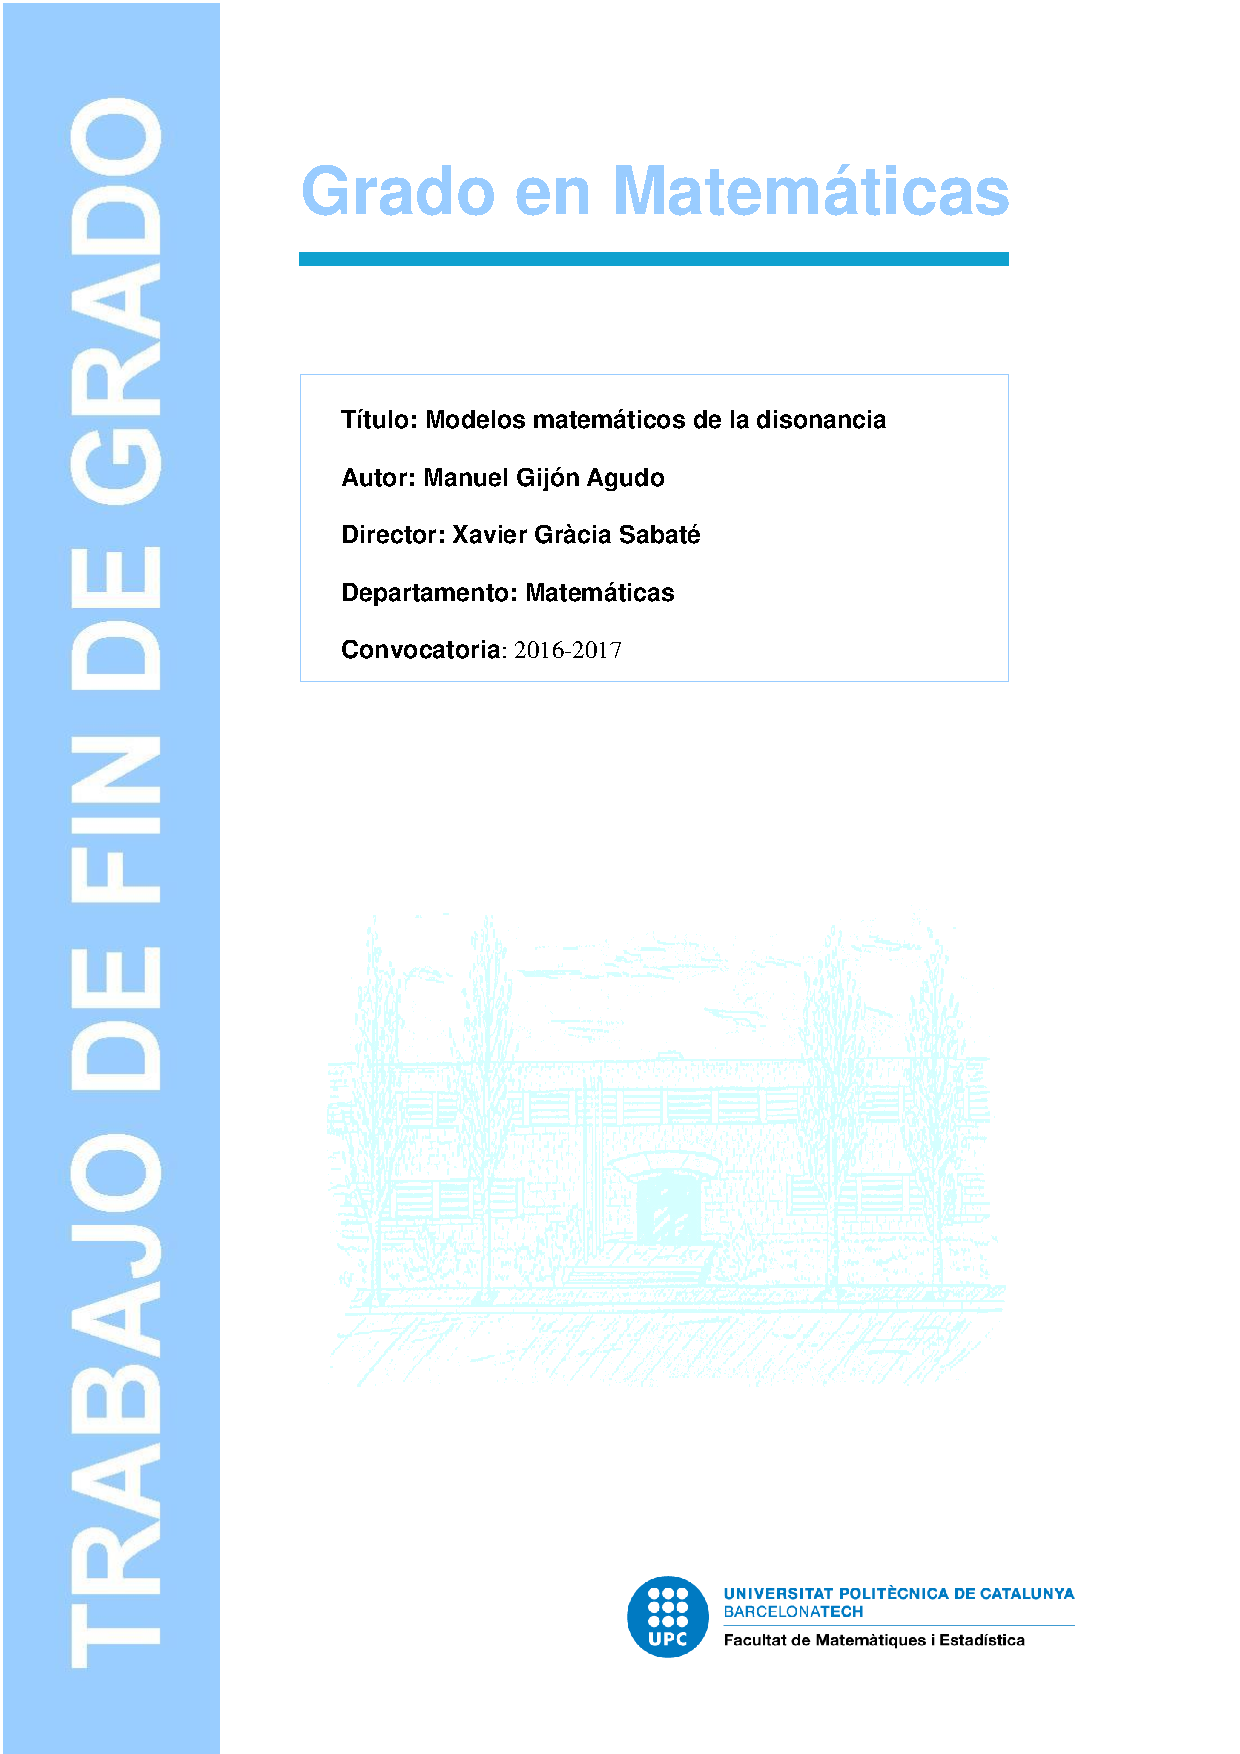
\includepdf{Portada.pdf}

\clearpage\null\thispagestyle{empty}\newpage % PÁGINA EN BLANCO ANTES DEL TÍTULO

%%%%%%%%%%%%%%%%% TÍTULO %%%%%%%%%%%%%%%%%%%%%%%%%%%%%%%%%
\pagenumbering{roman} %This command sets the page numbers to lowercase Roman numerals.

\maketitle{}
\thispagestyle{empty} % Elimina la numeración de esta página
\newpage

%Ahora añadiré una página en blanco sin numerar...
\clearpage\null\thispagestyle{empty}\newpage

% No es posible añadir páginas en blanco sin contenido, de ahí la última línea



%\pagenumbering{roman} %This command sets the page numbers to lowercase Roman numerals.

%%%%%%%%%%%%%%%   RESUMEN   %%%%%%%%%%%%%%%%
\addcontentsline{toc}{section}{Resumen}
\vspace{3cm}
\noindent\Large{\textbf{Resumen}}\\
\normalsize

\noindent\textbf{Palabras clave:} ondas, sonido, afinación, escalas, espectro, disonancia\\

\noindent\textbf{MSC2010:} 00A65, 00A06 00A17, 97M80\\ % Mathematics and Musicm; mates para no matematicos; External book reviews; arts, music, lenguaje and architecture

%\vspace{1.2cm}

El objetivo principal de este trabajo es estudiar los modelos matemáticos conocidos como curvas o superficies de disonancia que nos permiten estudiar el fenómeno perceptivo de la disonancia. La motivación del trabajo es establecer nuevos teoremas sobre estos modelos que, bajo unas condiciones razonables que también estableceremos, nos proporcionen resultados útiles para entender el comportamiento del fenómeno.
\\*
También se revisan las distintas explicaciones del fenómeno de la disonancia a lo largo de la historia, su relación con la construcción de escalas, los distintos métodos de afinación y las diferencias entre las visiones físicas y los enfoques perceptivos en el estudio del sonido.


%\newpage
%\clearpage\null\thispagestyle{empty}\newpage % Página en blanco
    \vspace{2.5cm}

\addcontentsline{toc}{section}{Abstract}
\vspace{3cm}
\noindent\Large{\textbf{Abstract}}\\
\normalsize

\noindent\textbf{Keywords:} waves, sound, tuning, scales, spectrum, dissonance\\

\noindent\textbf{MSC2010:} 00A65, 00A06 00A17, 97M80\\ 

The main objetive of this bachelor thesis is to study the mathematical models known as curves o surfaces of dissonance that allow us to study the perceptive phenomenon of dissonance. The goal of this paper is to establish new theorems about this models that, under under certain reasonable condictions that we have to establish too, give us useful resoults in order to understand the behavior of the phenomena.
 \\*
Also, different explanations that are been given to the phenomena of dissonance in history are explained, its relation with the construction of a musical scale is exposed, different methods of tuning and the differences between a physical or a perceptive approach to the study of the sound are discussed too.

\newpage
\clearpage\null\thispagestyle{empty}\newpage % Página en blanco

%%%%%%             ÍNDICE          %%%%%%%%%%%%%%


\tableofcontents
\newpage


%Ahora añadiré una página en blanco sin numerar...
%\clearpage\null\thispagestyle{empty}\newpage
\addcontentsline{toc}{section}{Prefacio}
\section*{Prefacio}


    Hace un par de años, en la Universidad Autónoma de Madrid, cursé la asignatura de Ecuaciones en Derivadas Parciales de la mano del profesor Juan Ramón Esteban. Junto con las interminables hojas de ejercicios que nos hacía llegar cada semana, se acompañaba una hoja con las referencias bibliográficas oportunas. Y en una de estas, entre clásicos del tema como los libros de Salsa o de Strauss se encontraba un libro que llamó mi atención: ``Music. A mathematical offering'' de D.J. Benson. No me resultaba nueva la relación entre música y matemáticas, ya había oído sobre el tema en documentales y trabajos de divulgación como los realizados por Marcus du Sautoy, sin embargo, no había podido imaginar que hubiera trabajos sobre el tema tan complejos y profundos.
    
    Años después me encuentro acabando la carrera en Barcelona. Cuando me enfrenté a la búsqueda de un trabajo de final de grado que me interesase, me encontré con una sorpresa inesperada. No podía imaginar que entre la oferta de trabajos se encontrasen trabajos sobre música. Desde que leí por primera vez sobre el tema, tenía ganas de profundizar en la relación entre música y matemáticas, por azares del destino ahora tenía esa oportunidad. Contacte con el profesor Xavier Gràcia Sabaté, el único que ofertaba esta clase de trabajos, en diciembre del pasado año y tras acceder a dirigirme el trabajo, nos pusimos manos a la obra.
    
    Me gustaría agradecer especialmente a este profesor, Xavier Gràcia Sabaté, su ayuda e infinita paciencia. El propio hecho de que aceptase dirigirme el trabajo sin conocerme de nada, recién llegado a la FME, y sin experiencia ni en \LaTeX{} ni en la redacción de trabajos académicos es un hecho, por sí mismo, a agradecer.
    
    Me gustaría también agradecer desde aquí a mi familia su inestimable apoyo. También aprovecho estas páginas para recordar, a modo de agradecimiento, a todas las personas implicadas en mi intercambio académico, el presente curso estudio como alumno de intercambio en el programa SICUE, desde mi coordinador en Madrid, José Ramón Berrendero, hasta la gente de gestión académica de la secretaría de la FME quienes, a pesar de volverles prácticamente locos con diversos problemas de papeleo, jamás perdieron la paciencia conmigo. En particular me gustaría darle las gracias a Jaume Soler Villanueva, quien me ayudó en el proceso de matriculación del presente trabajo que, debido a problemas burocráticos, dio más trabajo de lo habitual.
    
    Por último, me gustaría agradecer sinceramente a todos mis compañeros de la FME su cálida acogida, desde el primer día me han hecho sentir parte de la facultad sin apenas conocerme. Podría citar a muchos, pero me parecería, dado el trato que me han dado, demasiado grave olvidar tan solo a uno de ellos como para arriesgarme a cometer semejante error. Solamente me permitiré particularizar en un caso, quiero dar las gracias especialmente a Raquel Leandra Pérez por su ayuda que, en lo que al trabajo se refiere, me ha resultado vital en el uso de las herramientas necesarias para que este trabajo viera la luz.
    
        
\newpage
\clearpage\null\thispagestyle{empty}\newpage % Página en blanco



%%%%%%%%%%%%%%%%%%%%%%%%%%%%%%%%%%%%%%%%%%%%%%%%%%

\pagenumbering{arabic} % contador a cero, numeración arábiga



\section{Introducción}

La relación entre la música y las matemáticas es muy antigua. De los chinos, los egipcios, y los mesopotámicos se conservan observaciones al respecto. Aunque fueron los pitagóricos los primeros en establecer la relación entre escalas musicales y las razones matemáticas de proporcionalidad entre los objetos físicos implicados en producir las distintas notas..
\\*
Se cuenta que tal era la obsesión de Pitágoras de Samos, siglo VI a.C., por encontrar los principios racionales sobre los que descansa el concepto de disonancia, que Nicómaco, siglo II d.C., cuenta sobre él la leyenda de los martillos. Esta historia describe como él, Pitágoras, mientras paseaba por la calle, al escuchar el ruido de los diferentes martillos golpeando contra los yunque en una herrería cercana, cayó en la cuenta de que dichos sonidos estaban afinados en relación al tamaño de los martillos. 
\\*
Este hecho en el caso de los martillos es falso, sin embargo, si es cierto en el caso de cuerdas. Si es cierto que una cuerda vibrante emite un sonido a un octava de distancia del que emite una curda cuya longitud sea la mitad de la original. También es cierto, que si la razón entre las longitudes de las cuerdas es de $3:2$, la nota emitida estará a distancia de una quinta. De este modo se establecieron las razones entre los diferentes sonidos de la escala y su relación con el mundo físico.

\\*
Llegados a este punto, es importante pensar que cómo se construyen las escalas. Una escala musical es un conjunto de sonidos ordenados en base a su altura en relación a una cierta nota fundamental. Como comentaremos más adelante, siempre es posible ordenar dos sonidos en términos de cuál es más grave y cuál es más agudo, esto es, en base a cual sea su altura. Pero la pregunta sigue en el aire, ¿por qué hemos tradicionalmente escogido unos sonidos en lugar de otros de entre el infinito rango de sonidos posibles ? La respuesta a esta pregunta es simple: de entre los infinitos posibles sonidos a escoger estos y no otros son los que producen menor disonancia.

\\*
Ahora nos surge otra pregunta: ¿qué es la disonancia?. Según la Real Academia de la Lengua Española, la disonancia, término que procede del latín dissonantia, se define como:

\begin{textsl}

    \item f. Sonido desagradable.
    \item f. Falta de la conformidad o proporción que naturalmente debe tener algo.
    \item f. Música. Acorde no consonante.
    \item locución verbal. Parecer extraño y fuera de razón.

\end{textsl}
\\*
\vspace{.80cm}
Por tanto, de entre las posibles notas o sonidos a escoger para conformar nuestras escalas hemos escogido tradicionalmente aquellas que no nos resultan desagradables al escucharlas juntas. Aquellas que minimizan la disonancia.\\*

En nuestro análisis, calcularemos la disonancia mediante unos modelos matemáticos concretos. Si calculamos la disonancia entre dos notas estaremos ante \emph{curvas de disonancia}, si la calculamos entre tres sonidos tendremos \emph{superficies de disonancia} y cuando lo hagamos para más sonidos interaccionando, \emph{superficies de disonancia de dimensiones mayores}. En dimensiones mayores el razonamiento es análogo, sin embargo, centrémonos en las curvas. Cuando calculemos la curva lo haremos en base a un parámetro al que llamaremos generalmente $\alpha$ que representa la razón entre la nota fundamental, aquella no no variará, y las notas que interactuarán con ella. Esta curva tendrá unos máximos y mínimos, puntos que interpretamos como más o menos disonantes. A la hora de construir una escala, escogeremos notas situadas a las razones de la fundamental en las que se encuentran los mínimos de la curva, aquellas notas menos desagradables al oído.
\\*
Otra pregunta pertinente sería: ¿es la disonancia un efecto puramente físico producido por la interacción de los elementos físicos que conforman estos sonidos, o es un elemento cultural que hemos aprendido mediante aprendizaje vicario? Dicho de otra forma, ¿es la disonancia entro dos sonidos independiente de la cultura a la que pertenezcan los individuos que los identifiquen como desagradables? Es una pregunta importante, a lo largo de este trabajo veremos diferentes teorías al respecto, aunque nos centraremos en aquellas que consideran la disonancia un proceso eminentemente físico y excluiremos las teorías que los consideran, en mayor medida, un elemento fruto de la interacción social y cultural.
\\*
Una vez tenemos claro el objeto a estudiar, la siguiente pregunta que cabe hacernos es cómo vamos a estudiarlo. Para estudiar la disonancia deberemos encontrar alguna forma de medirla. Alguna forma de poner sobre el papel cuán disonantes son dos sonidos. Si bien no podremos hacerlo de manera absoluta, al menos trataremos de hacerlo de manera relativa, de entre dos situaciones donde se nos presenta disonancia podremos decir en cuál de ellas lo hace con mayor intensidad.

\subsection{Objetivos}

El objetivo principal de este trabajo es el estudio establecimiento de nuevos teoremas sobre los modelos utilizados para modelizar el fenómeno de la disonancia.
Estos modelos consisten en las llamadas \emph{curvas de disonancia}, curvas que nos indican cuán disonante es un sonido en relación a otro cuya frecuencia fundamental del espectro se sitúa a una distancia determinada. En este trabajo consideraremos el caso en que estos sonidos tienen espectros igualmente distribuidos.

Para alcanzar el objetivo, daremos una definición más general que la aportada por Sethares de qué es una curva de disonancia y sobre esta, será sobre la que estableceremos los nuevos teoremas. Esta definición sirve además para modelizar diferentes datos, más allá de ajustarse bien únicamente a los obtenidos por Plomp y Levelt.

Otro de los objetivos es el mejor entendimiento del modelo propuesto por Sethares. Para ello, establecemos dos nuevos resultados sobre el núcleo de las curvas de disonancia utilizadas por el autor, las llamadas \emph{Curvas de Plomp-Levelt} (que son utilizadas por él como \emph{funcione de disonancia}, aquella que dada una distancia medida de una forma concreta entre dos frecuencias da como resultado su disonancia).

El último de los objetivos es aportar una breve visión histórica sobre cómo ha evolucionado el concepto de disonancia.

\subsection{Contenidos}

A continuación procedemos a describir con detalles los contenidos de cada capítulo.

En el segundo capítulo haremos especial hincapié en las diferencias entre las visiones físicas y los enfoques perceptivos en el estudio del sonido. Este, al ser la noción de disonancia algo perceptivo, será uno de los contenidos claves para entender el presente trabajo. Este capítulo estará centrado por tanto, en entender bien que conceptos como espectro y timbre, intensidad y sonoridad o frecuencia y altura si bien están íntimamente relacionados no son exactamente lo mismo y que responden a diferentes maneras de enfocar el estudio del sonido.\\*
Daremos también algunas explicaciones sobre el por qué existen los diferentes métodos de afinación y a cuáles son sus ventajas y desventajas.
\\*

El tercer capítulo se centra en tratar el fenómeno de la disonancia y distintas explicaciones del mismo. Haremos un breve repaso histórico del estudio del fenómeno. Mención especial merecen en las justificaciones de Helmholtz y su teoría de los batidos y las de R.Plomp y W.J.M.Level. La teoría de Helmholtz se basaba en la forma de la interacción resultante de sumar dos ondas individuales. Plomp y Levelt se encargaron de elaborar una nueva teoría que mejoraba la enunciada por Helmholtz.

\\*

En el cuarto capítulo se encuentra el núcleo del trabajo. Se incluye el análisis hecho por Sethares del modelo basado en las curvas de Plomp-Levelt en la primera parte, así como dos observaciones sobre este modelo que el autor no hizo. La segunda parte del capítulo desarrolla un resultado general sobre las curvas de disonancia. El resultado permite asegurar el unísono como mínimo de la curva en un contexto más amplio que el contemplado por Sethares, dentro del marco establecido por la definición dada de curva de disonancia.
\\*


El apéndice está dedicado a incluir información adicional sobre temas tratados en el resto del trabajo. Así mismo, se incluye la demostración de Sethares de que unísono es un mínimo de la curva  de disonancia y la explicación de por qué esta demostración no es correcta. Notemos que el resultado general aportado en la segunda parte del anterior capítulo asegura que este resultado también sera cierto.\\*

\subsection{Recursos utilizados}

Los recursos en los que se fundamente este trabajo son, fundamentalmente, los libros de Sethares \cite{Set} y el de Benson \cite{Bens}. También es importante el artículo de R. Plomp y W. M. Levelt en relación a las gráficas de disonancia \cite{PL}.

El software fundamental es Matlab. Con él se han hecho todas las gráficas de curvas de disonancia incluidas en el trabajo. En el apéndice se incluyen los programas con los que hacer dichas gráficas así como el programa con el que, dado un espectro concreto, crear archivos de audio. Algunos de los gráficos se han realizado con TikZ, un entorno de \LaTeX{} que permite hacer toda clase de figuras y esquemas.

En el apéndice, en la sección número $3$, se exhibe un cálculo hecho con el software R y programado en el lenguaje homónimo. Este software y su manejo no es esencial, el mismo cálculo podría repetirse en Matlab o, con paciencia, incluso en una calculadora.


\subsection{Conclusiones}

Se han estudiado las curvas de disonancia y sus propiedades.

Se han obtenido nuevos resultados sobre las curvas estudiadas por Sethares, un marco general en el que definir qué es una curva de disonancia y que no y un teorema general enmarcado dentro de este contexto que nos asegura que para espectros con un número arbitrario de parciales el unísono será un mínimo de la curva de disonancia.

Sería apropiado insistir en la idea de que el concepto de disonancia y extremadamente amplio y toca diferentes ramas del saber, desde la matemática o la física, hasta la psicoacústica o la sociología. Su estudio, por tanto, debería hacerse desde muchos ángulos. En el presente trabajo solamente hemos hablado de los modelos que se utilizan, para acercarse a la disonancia desde el punto de vista matemático. No hemos hablado ni de cómo se extraen los datos para confeccionarlos, ni de cómo estos pueden variar dependiendo de los sujetos involucrados, ni de otros muchos conceptos cuyo estudio bien merecería sendos trabajos similares a este. Tampoco, por la extensión del trabajo, hemos podido incluir el estudio de superficies de disonancia, modelos producidos a partir de la interacción de tres sonidos sonando simultáneamente, ni de superficies de dimensión mayor, que quizás, por lo complejo que son en realidad los sonidos que verdaderamente escuchamos en nuestro día a día, serían de gran interés. Mención a parte merecen los casos más complejos aún, aquellos en que los espectros de los sonidos implicados son diferentes. Seguramente, el teorema global enunciado en este trabajo sirva en el futuro para estudio de dichas superficies y casos más complejos, pero por el momento, sirvan los contenidos del presente trabajo como una introducción al estudio, desde el punto de vista matemático, del fenómeno de la disonancia.



\newpage


%%%%%%%%%%%%%%%%%%%%%%%%%%%%%%%%%%%%%%%%%%%%%%%%%%%%%%%%%%%%
\section{El sonido y la percepción del mismo}

%		\newtheorem{Teorema}
%   \par nuevo párrafo
%    línea en blanco -> párrafo nuevo
%	-puntuación dentro del doble dolar -> espacios matemñaticos% \, \: \;	 de menor a mayor
%   CTAN -> información paquetes

	\subsection{Sonido}
	
	    Según la Real Academia de la Lengua Española, el sonido se define como:
	    
	    \begin{center} 
	    `` Sensación producida en el órgano del oído por el movimiento vibratorio de los cuerpos, transmitido por un medio elástico, como el aire.''
	    \end{center}
	    
		Otra posible definición atiende a aspectos perceptivos:

		\begin{center}
		``La sensación generada en los órganos audioperceptivos por vibraciones en el aire o en otro medio''\cite{Set}.
		\end{center}
		
		 A partir de las anteriores definiciones, podemos ver que el término "sonido" puedo aplicarse a dos aspectos muy diferentes de lo que es un mismo fenómeno, por un lado el aspecto físico (cuantificable y objetivo) y por otro de psicólógico (eminentemente subjetivo).
		 \vspace{3mm}

		Pero, ¿cómo se transmite el sonido?. Lo hace por el aire, o por cualquier otro medio elástico, en forma de cambios en la presión del mismo. En el caso del aire y otros medios lo hace mediante cambios en la concentración o densidad de sus moléculas. La ecuación que modeliza el movimiento armónico simple, el tipo de movimiento que sigue este fenómeno, es:
		
		$$ \cfrac{d^2y}{d t^2} = -ky $$ 
		Cuya solución general es:
		$$ y = A \cos(\sqrt{kt}) + B \sin(\sqrt{kt})$$
		Equivalentemente:
		$$ y = c \sin(\sqrt{kt} + \phi) $$
		
		En este caso estaríamos hablando de una onda de \emph{frecuencia} $\nu = \frac{k}{2\pi}$ (que mediremos en Herzios), \emph{amplitud} $c$ y \emph{fase} $\phi$. Por comodidad reescribiré la expresión en términos de la frecuencia: $ y = c \sin( 2 \pi \nu t + \phi ) $.La cantidad $2\pi\nu$ también es llamada \emph{velocidad angular de la onda}. El papel que juega la fase es el de indicarnos en que punto la onda corta el eje temporal. Por ejemplo, una onda de expresión $ cos(x) = sin(x + \frac{\pi}{2} )$, es decir, una onda expresada mediante el coseno es idéntica a una expresada mediante el seno pero con una con un desplazamiento de $\frac{\pi}{2}$ unidades en el eje espacial.
		
		Por ejemplo, convencionalmente, la nota La situada bajo el Do central se sitúa a una frecuencia de $440$ Hz, es decir, que podemos representarla utilizando la siguiente expresión: $ y = c \sin( 880 \pi t + \phi) $. 
		
		Podemos, en cualquier caso, no solo en este particular, convertir la expresión en una combinación lineal de senos y cosenos haciendo uso de las siguientes identidades :
		$$
			\sin ( A + B ) = \sin A \cos B + \cos A \sin B 
		$$

		$$
			\cos ( A + B ) = \cos A \cos B - \sin A \sin B
		$$
		
		Así obtenemos:
		$$
			c \sin (\omega t + \phi) = a \cos (\omega t) + b \sin (\omega t)
		$$
		
		donde		
		$$
			a = c \sin(\phi)     $$  $$        b = c \cos(\phi)
		$$
		
		Por otro lado tenemos:
		$$
			c = \sqrt{a^2 + b^2}  $$  $$  tan (\phi) = a / b 
		$$
		 
		\begin{figure}[h]  % h = aquí		
			\centering	
			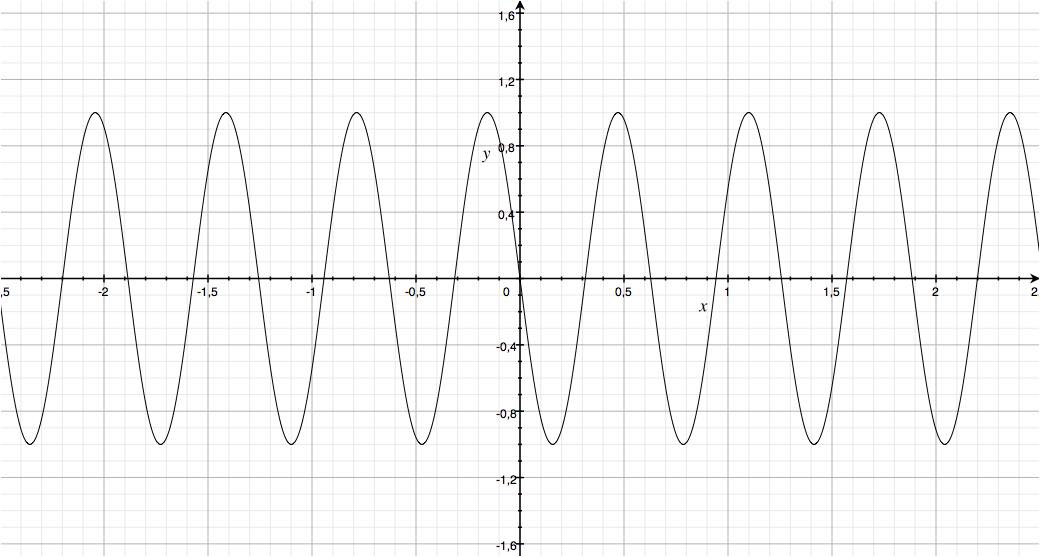
\includegraphics[scale= 0.3]{Sin10xmaspi.jpg}
			\caption{$ \sin(10x + \pi) $} 
		\end{figure}
	
		 Cuando se escucha una sola única onda sinusoidal, la \emph{ampitud} (fenómeno físico) está intensamente relacionada con el \emph{volumen} (fenómeno perceptivo) y la \emph{frecuencia} (fenómeno físico) directamente relacionada con el \emph{timbre} (fenómeno perceptivo).  Cuando el número de ondas que son escuchadas simultáneamente es igual o superior a dos, se producen nuevos fenómenos perceptivos, como pueden ser las interferencias constructivas o destructivas entre las ondas debidas a la relación entre las fases de las mismas. Los batidos (fenómeno al que me referiré después) son producidos cuando las frecuencias de estas ondas difieren y sensorialmente pueden ser percibidos como disonancia.
		 
		 En el siguiente ejemplo se pueden apreciar ambos tipos de interferencias, que dan lugar, en su envolvente, a una nueva onda sinusoidal de un periodo mayor que las anteriores:
		 
		 \begin{figure}[h]
		 	\centering
		 	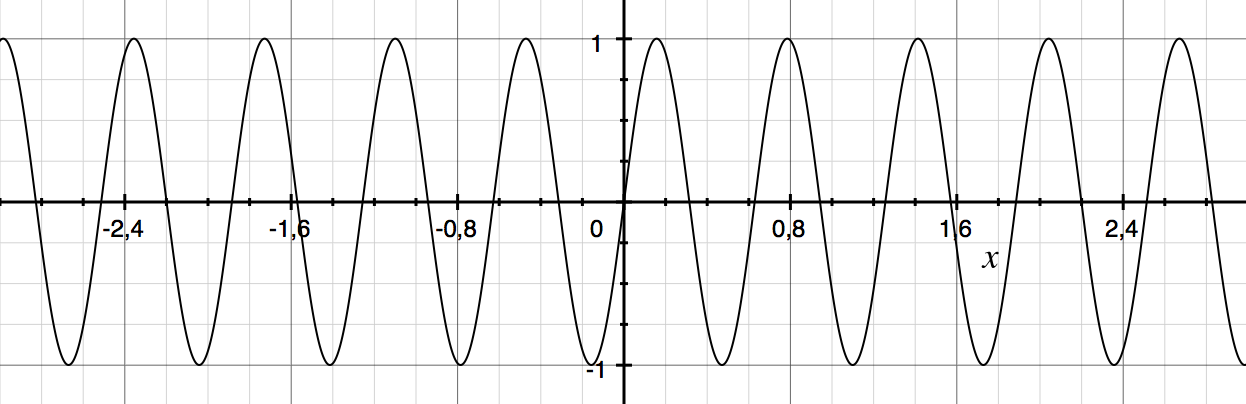
\includegraphics[scale=.4]{S31}
		 	\caption{$\sin(10 x)$}
		 \end{figure}
		 
		 \begin{figure}[h]
		 	\centering
		 	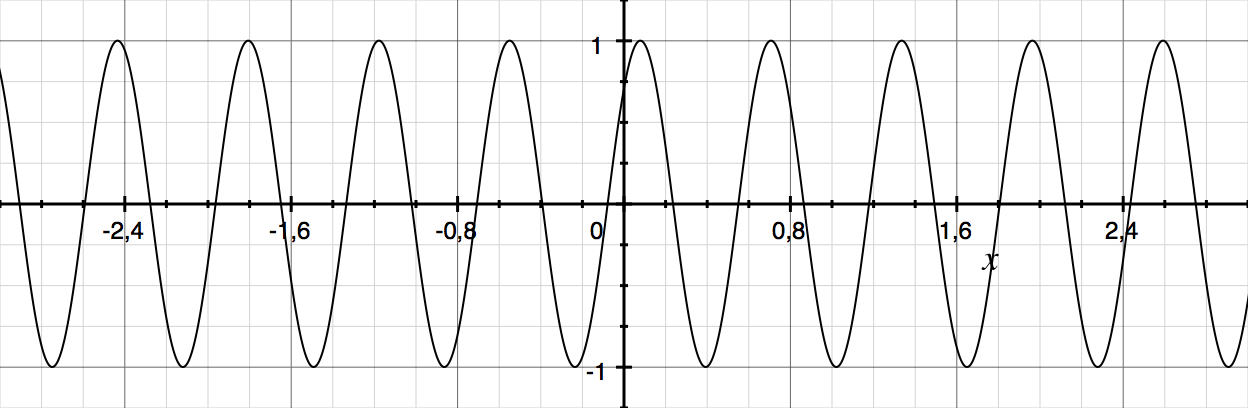
\includegraphics[scale=.4]{S32}
		 	\caption{$\sin(10 x + \frac{\pi}{4})$, la función anterior con una diferencia de fase $\phi = \frac{\pi}{4}$}
		 \end{figure}
		 
		 \begin{figure}[h]
		 	\centering
		 	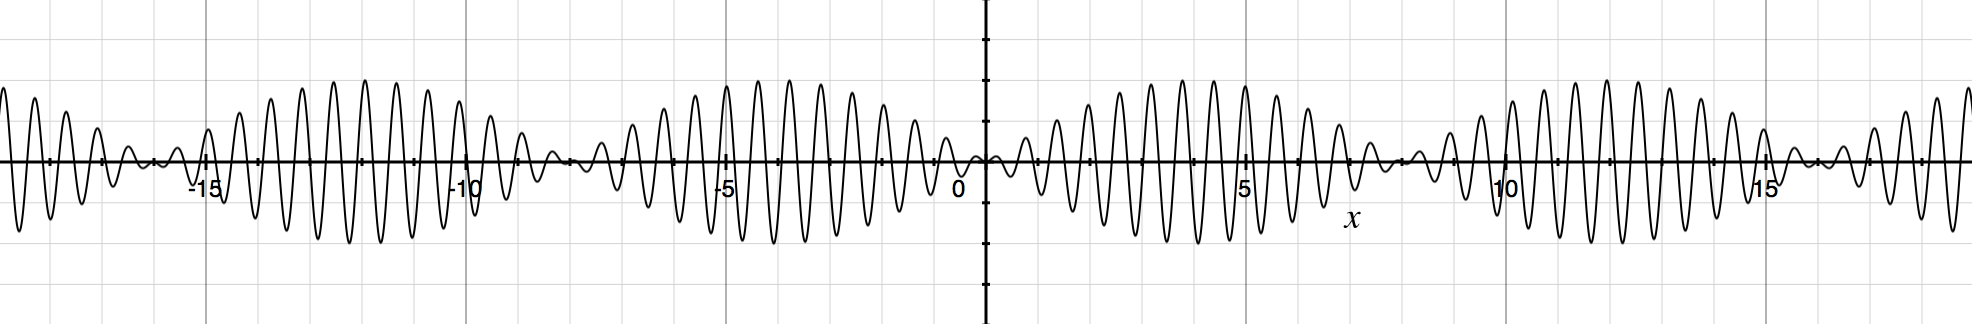
\includegraphics[scale=.4]{S34}
		 	\caption{$2 \sin(\frac{\pi}{8} x) \sin((10 + \frac{\pi}{8}) x)$, la función suma de las anteriores. Observemos como la envolvente de esta se corresponde de nuevo con una función sinusoidal.}
		 \end{figure}
		 
	%	 En los siguientes apartados discerniremos las diferencias entre los fenómenos físicos y sus correspondientes percepciones.
		
	\subsection{Espectro y timbre}
	
	Pensemos en como se descompone un rayo de luz al atravesar un prisma dando lugar a los colores del arco iris. Esto ocurre porque el rayo está compuesto, aunque no sea evidente, por diferentes ``colores'' que se diferencian entre ellos entre otras cosas porque los rayos que les dan lugar tienen diferentes índices de refracción. Este fenómeno es lo que hace que al atravesar el prisma en ángulo con el que salen de él sea diferente (Ley de Snell).
	 
	 De la misma manera, una misma onda sonora se descompone en diferentes ``colores'', cada uno de ellos será una onda diferente, con una frecuencia, amplitud y fase propias y que la caracterizan. Estos ``colores'' son las denominadas \emph{parciales} o \emph{armónicos}. El conjunto de estas parciales es lo que se denomina \emph{espectro}.
	 
	 Por seguir con la analogía, es este caso nuestro prisma sería la llamada \emph{Transformada de Fourier}, o más concretamente, al implementarlo en un ordenador, la Transformada Discreta de Fourier (DFT, Discrete Fourier Transform) y la Transformada Rápida de Fourier (FFT, Fast Fourier Transform).
	 
	 
	 Intuitivamente, el \emph{espectro} de un sonido cualquiera es un gráfico en el que están representadas las amplitudes de las diferentes frecuencias en el sonido.
	 
	 Un caso simple es el espectro de una cuerda vibrante de frecuencia fundamental $ \nu = \sqrt{k / m} / (2 \pi)$:
	 
	 \begin{figure}[h]
	     \centering
	       \begin{tikzpicture}[scale = 2.25]
	            \draw[thick, <->] (0,2) -- (0,0) -- (5,0);
	            \node [left] at (0,2) {amplitud};
	            \node [below] at (5,0) {frecuencia};
	            \draw (1,1.75) -- (1,0);
	            \node [below] at (1,0) {$\nu$};
	            \draw (2,1.25) -- (2,0);
	            \node [below] at (2,0) {$2 \nu$};
	            \draw (3,1) -- (3,0);
	            \node [below] at (3,0) {$3 \nu$};
	            \draw (4,.5) -- (4,0);
	            \node [below] at (4,0) {$4 \nu$};
 	       \end{tikzpicture}
	     \caption{Espectro discreto de una cuerda vibrante}
	 \end{figure}
	 
	 Este gráfico ilustra un sonido con un espectro discreto de frecuencias cuyos componentes son múltiplos enteros de la frecuencia fundamental y cuyas respectivas amplitudes decaen con el aumento de las mismas. Algunos sonidos, como el denominado \emph{ruido blanco} no poseen un espectro discreto, si no continuo. Es este caso además la amplitud no decae con el aumento de frecuencias.
	 
	 
	\begin{figure}[h]
		\centering
			\begin{tikzpicture}[scale = 2.75]
				\draw [thick,<->] (4,0) -- (0,0) -- (0,2);
				\draw (0,1.25) -- (4, 1.25);
				\node [below] at (2, 0.90) {Ruido blanco};
				\node [left] at (0,2) {amplitud};
				\node [below] at (4,0) {frecuencia};
			\end{tikzpicture}
		\caption{Espectro del denominado ruido blanco}
	\end{figure}	 
	 
	 Presentemos ahora la definición de \emph{timbre} que considera la Real Academia Española:
	 
	 \begin{center}
	 ``Cualidad de los sonidos determinada por el efecto perceptivo que produce en los oyentes.''
	 \end{center}

     El American National Standards Institute \cite{ANSI} añade a la definición de timbre una característica de gran utilidad:
     
	 \begin{center}
	 ``El timbre es el atributo de la percepción sonora en términos del cual el oyente puede distinguir entre dos sonidos presentados de la misma forma  de igual volumen y altura''.
	 \end{center}

	La definición dada por Pratt and Doak \cite{PD} apoya la anterior, añadiendo además que la duración de las notas tampoco es relevante a la hora de que el timbre nos permita distinguir entre dos sonidos. 	
	
%	``El timbre es el atributo de la sensación sonora mediante el cual el oyente puede distinguir entre dos sonidos sin atender a su altura, volumen o duración.''
	Enric Herrera, en el primer volumen de su libro ``Teoría musical y armonía moderna''\cite{EH}, hace especial énfasis en que, además de permitirnos distinguir entre dos sonidos, el timbre también es característico de cada instrumento o familia de instrumentos al estar relacionado con los armónicos concretos generados por los mismos.
		 
	 \begin{center}
	 	``El timbre es aquella cualidad de un sonido que nos hacer poder distinguirlo de otro de la misma altura. Cada instrumento o familia de instrumentos tiene un timbre característico, que está directamente relacionado con los armónicos (ver serie armónica) que produce dicho instrumento. Ningún instrumento produce un sonido, llamémoslo puro o simple, sino una serie de sonidos que nos llegan en conjunto como una nota.''
	 \end{center}
	 
	 En el mismo libro, se expone también la relación entre el timbre y los diferentes parciales del sonido, el espectro del mismo:
	 
	 \begin{center}
	 	``Una nota musical es un sonido compuesto por una serie de sonidos simples. La descomposición de un sonido compuesto en un grupo de sonidos parciales o concomitantes, se llama serie armónica. El número y la intensidad de los sonidos concomitantes determinan el timbre.''
	 \end{center}
	 
	 En cualquier caso ninguna de estas definiciones ni de otras posibles reflejan la importancia de factores como el ataque o el decaimiento de los sonidos en el timbre de los mismos.
	 Por tanto, podríamos decir que timbre y espectro están íntimamente relacionados, el timbre no es arbitrario, sino que está condicionado por otros factores que no son el únicamente espectro. A mismo espectro, una misma pieza musical tocada al revés comparte espectro con la versión original, por ejemplo, sin embargo el timbre de ambas es diferente.
	 
	\subsection{Intensidad y sonoridad}
	
	De nuevo, a la hora de buscar una definición desde la que comenzar a estudiar un sonido, recurrimos a la Real Academia de la Lengua:
	
	\begin{center}
	    ``Magnitud física que expresa la mayor o menor amplitud de las ondas sonoras, y cuya unidad en el sistema internacional es el fonio.''
	\end{center}
	
	La definición que de E. Herrera \cite{EH} de \emph{intensidad} es la siguiente:
	
	\begin{center}
	``Intensidad: Es la cantidad de sonido emitido, asimilable a la potencia. La intensidad no es igual en los distintos instrumentos, ni lo es en todo el registro de un mismo instrumento.
	
	La intensidad de una nota o frase se regula por medio de las dinámicas. Esta cualidad acústica es muy importante para una adecuada orquestación, ya que dos instrumentos de familia distinta tocando la misma melodía la misma altura y con el mismo dinámico no tendrán la misma intensidad y uno puede hacer desaparecer al otro o crear un efecto indeseado.''
	\end{center}
	
	Atendamos ahora al concepto físico: la intensidad de sonido se define como la potencia acústica (cantidad de energía por unidad de tiempo, potencia, transmitida por la onda al propagarse en un determinado medio) por unidad de área normal a la dirección de propagación.
	
	$$
		\hbox{Intensidad} = \frac{\hbox{Potencia acústica}}{\hbox{Área normal a la dirección de propagación}}
	$$
	
	Esta magnitud se mide en el Sistema Internacional de Unidades en vatios por metro cuadrado ($ W / m^2$). El oído humano tiene la capacidad de escuchar sonidos, normalmente, desde los $10^{-12} W/m^2$ (frecuencia conocida como \emph{umbral de audición}). Cuando la intensidad supera $1 W/m^2$ la sensación producida se vuelve,generalmente, dolorosa.
	
	Así por ejemplo, la intensidad sonora producida en el espacio, propagándose en todas direcciones a la misma velocidad (con lo que su frente de ondas, o conjunto de puntos del espacio a los que llega la onda en un mismo instante de tiempo, será una esfera, pongamos que de radio $r$) será: 
	
	$$
	I = \frac{P}{N} = \frac{P}{4\pi r^2}
	$$
	
	Como consecuencia de que en el rango de intensidades que el oído humano puede aceptar sin dolor es grande, por comodidad se emplea una escala logarítmica. Por convección, en dicha escala se emplea como referencia el umbral de audición. La unidad de medida más empleada es el \emph{decibelio}.
	
	$$
		B_{dB} = 10 \log_{10} \left( \frac{I}{I_{0}} \right)
	$$
	
	Donde $B_{dB}$ es el nivel de intensidad sonora en decibelios, $I$ la intensidad sonora en escala lineal (medida en $W/m^2$) y $I_{0}$ es el umbral de audición ($10^{-12} W/m^2$).

	
	\begin{figure}[h]
	    \centering
	    \begin{tabular}{|c|c|}
	        \hline
	        200 dB & Bomba atómica similar a las explosionadas en Hirosima y Nagasaki \\ \hline
	        180 dB & Cohete durante el despegue \\ \hline
	        140 dB & Umbral del color. Coche de Fórmula 1 \\ \hline
	        130 dB & Avión durante el despegue \\ \hline
	        120 dB & Motor en marcha \\ \hline
	        110 dB & Concierto \\ \hline
	        100 dB & Perforadora eléctrica \\ \hline
	        90 dB & Tráfico \\ \hline
	        80 dB & Tren \\ \hline
	        70 dB & Aspiradora \\ \hline
	        50 dB & Aglomeración de gente \\ \hline
	        60 dB & Lavaplatos \\ \hline
	        40 dB & Conversación normal \\ \hline
	        20 dB & Biblioteca \\ \hline
	        10 dB & Respiración tranquila \\ \hline
	        0 dB & Umbral de audición  \\ \hline	        	        
	    \end{tabular}
	    \caption{Niveles de intensidad de diversos sonidos en decibelios}
	\end{figure}
	
	Sin embargo, la \emph{sonoridad} es la medida subjetiva de la intensidad con la que un sonido es percibido por el oído humano. Es decir, es la medida que nos permite ordenar de mayor a menor intensidad una serie de sonidos. Su unidad de medida es el \emph{fon} o \emph{fonio}.
	
	El fon se define como la sonoridad de un sonido sinusoidal de $1 KHz$ con un nivel de presión sonora de $0 B_{db}$. 
	
	$$
		S = 10 \log_{10} \left( \frac{I}{I_{0}} \right)   \hbox{fonios}
	$$
	
	El fons es una unidad que no sirve para comparar sonidos.Para poder comparar dos sonidos se establece una nueva unidad, el \emph{son} o \emph{sonio}, que se define como la sonoridad de un sonido sinusoidal de $1 KHz$ con un nivel de presión sonora de $40 B_{db}$.
	
	Esta unidad está relacionada con la frecuencia de un sonido y con su intensidad por medio de las llamadas \emph{curvas isofónicas}. Estas curvas son curvas de igualdad sonora. Las primeras fueron establecidas por Munson y Fletcher en 1930, más tarde, fueron recalculadas por Robinson y Dadson. En ambos casos, estas curvas son válidas para un campo sonoro directo, es decir, no contemplan que los sonidos provengan de diferentes direcciones.
	
	\begin{figure}[h]
		\centering
		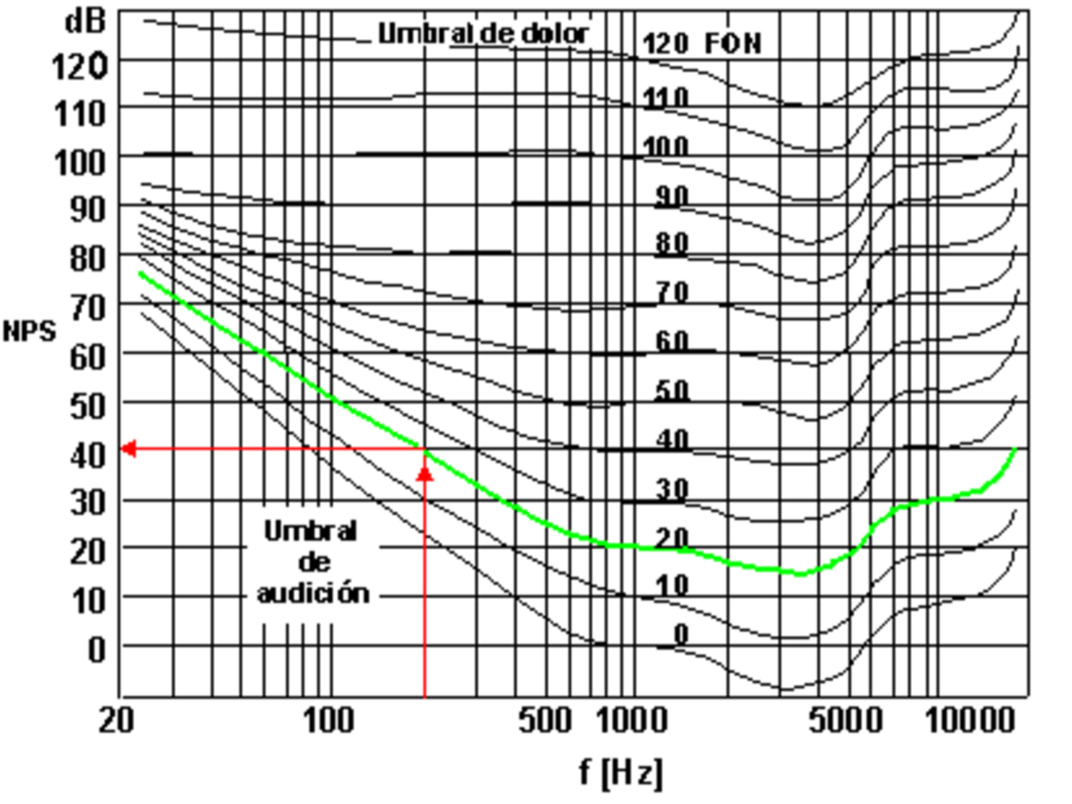
\includegraphics[scale=.4]{CurvasIso}
		\caption{Curvas isofónicas. NPS se corresponde con el nivel de presión sonora y f con la frecuencia expresada en Hz}
	\end{figure}
	
	
	En estas curvas (Figura 8) se observa como al aumentar la intensidad sonora las curvas se aplanan, lo que indica la dependencia de la frecuencia es mayor a medida que aumenta el nivel de la presión sonora. Esto implica que al disminuir la intensidad sonora los primeros sonidos en desaparecer serían los más graves, los que se corresponden con las frecuencias más bajas.
	
	\subsection{Frecuencia y altura}
		
		Tradicionalmente, y para ondas puras e instrumentos de cuerda y viento, se dice que la \emph{altura} percibida es al logaritmo de la \emph{frecuencia} de la señal.
		
		A Pitágoras de Samos se le adjudica el descubrimiento entre la relación entre la altura de la nota emitida por una cuerda al vibrar y su longitud, dándose que cuando la longitud de la cuerda es la mitad (relación 1:2) la nota producida está una octava por encima de la primera. Si ahora, partiendo de la misma cuerda, hacemos que vibren porciones de esta de razones 2:3 y 3:4 las notas emitidas serán respectivamente la quinta y la cuarta musicales respecto a la nota original ($7$ y $5$ semitonos de distancia respectivamente). Pitágoras y sus seguidores llegaron a describir todo el universo en función de relaciones armónicas simples. 
		
		La altura percibida a la que vibra la cuerda pitagórica es proporcional a la frecuencia con la que esta vibra. Es más, las alturas musicalmente más utilizadas no se definen en términos de frecuencias, sino en términos de razones de frecuencias. A estas razones es a lo que denominaremos \emph{intervalos musicales}.
		
		Ahora sí, pasemos a definir \emph{altura} \cite{ANSI}:
		
		%%%%%%%%%%%%%%%%%%%%%%%%%%%%%%%%%%%%%%%%%%%%%%%%%%%%%%%%%%%%%%%%%%%%%%%%%%%%%%%%%
		%			that attribute of auditory sensation in terms of which sounds may be ordered on a scale extending from low to high.                                      %
		%%%%%%%%%%%%%%%%%%%%%%%%%%%%%%%%%%%%%%%%%%%%%%%%%%%%%%%%%%%%%%%%%%%%%%%%%%%%%%%%%
		
		\begin{center}
		``atributo en términos de la sensación sonora que hace posible dotar de un orden, de bajo a alto, diferentes sonidos''
		\end{center}
				
		La siguiente definición de altura \cite{EH} nos aporta además información sobre cómo se distribuyen las notas en relación a su distancia en Hz y de sus posiciones respectivas:
				
			\begin{center}
			``Altura: Depende directamente de la frecuencia, cuanto más aumenta esta, más alto (agudo) será el sonido. El número de periodos por segundo que necesita un sonido para cambiar a siguiente de la escala cromática (semitono) depende de la altura de dicho sonido, así el LA de diapasón $440$ Hz necesita aproximadamente $30$ Hz para cambiar a Si bemol, en cambio un sonido con $3000$ Hz necesitará aproximadamente $200$ Hz para subir un semitono.
			
			Cuando se compara la altura de dos sonidos, en realidad se refiere a la distinta frecuencia entre ambos.
			
			$$
				\frac{f_1}{f_2} = \hbox{ intervalo }
			$$
			
			El oído humano medio puede oír sonidos comprendidos entre unos $20$ Hz y $16000$ Hz aproximadamente.
			\end{center}
			
		Como las ondas sinusoidales tienen frecuencias definidas inequívocamente (y estas dan lugar a la percepción de un sonido de un tono determinado) es posible establecer un orden entre varios sonidos atendiendo a las diferencias de altura entre sus tonos. Si tenemos un sonido de un tono desconocido, siempre podemos establecer un orden de forma no ambigua entre este y otros sonidos, llamando a la onda que tenga este tono desconocido onda \emph{tono del sonido}.		
				
	\subsection{Sistema auditivo}
	
	Con el objetivo de entender mejor el sonido necesitamos estudiar cómo es percibido por el oído humano.
	
	\begin{figure}[h]
		\centering
		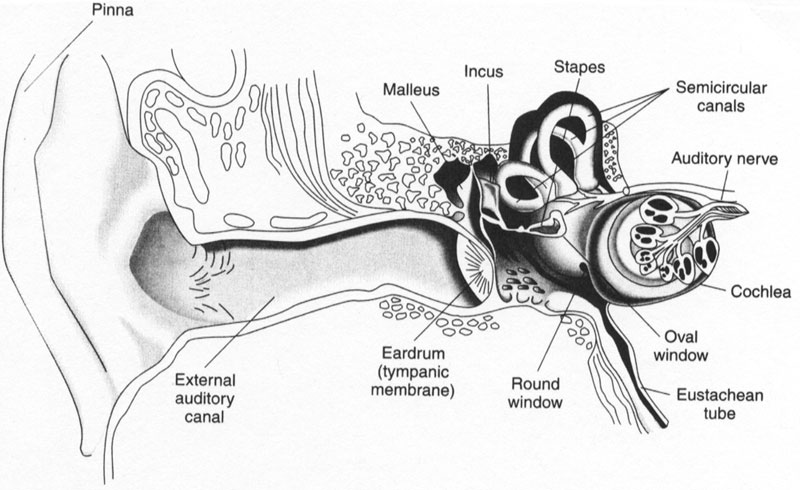
\includegraphics[scale=.3]{AuditorySystem.jpg} 
		\caption{Esquema del sistema auditivo}
	\end{figure}
	
	El  \emph{sistema auditivo} se divide en tres partes: 
	
	\emph{Oído externo}: Incluye el pabellón auditivo y el conducto auditivo externo. Está separado del oído medio por una fina membrana, el tímpano. El pabellón auricular se une a la cabeza mediante la piel y se compone principalmente de tejido cartilaginoso. La función principal del pabellón auditivo u oreja es canalizar las ondas sonoras, que atravesarán los $2,5 $mm de longitud media del conducto auditivo hasta llegar a la membrana timpánica (tímpano).
	
	\emph{Oído medio}: se encuentra excavado en el hueso temporal, uno de los ocho huesos del cráneo, formando una cavidad denominada caja del tímpano. Consiste en una cavidad llena de aire que contiene tres pequeños huesos (martillo, yunque y estribo) sujetos en por músculos y ligamentos. 	
	
	\begin{figure}[h]
		\centering
		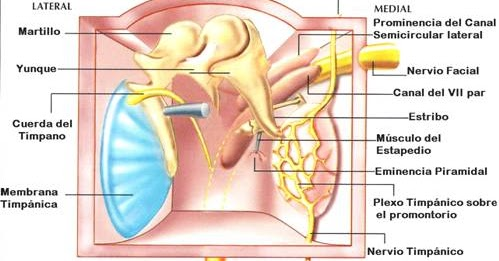
\includegraphics[scale=.6]{OMedio.jpg}
		\caption{Estructura del oído medio}
	\end{figure}
	
	En la pared que lo separa del oído interno hay dos pequeños orificios, la ventana oval y la ventana redonda. La base del estribo se asienta en la ventana oval, por donde se transmite el sonido al oído interno. La función de la ventana redonda es proporcionar una salida a las vibraciones sonoras.
	
	Existe otra estructura en el oído medio denominada trompa de Eustaquio que, con aproximadamente $1$mm de anchura y $35$mm de longitud, conecta el oído medio con la naso-faringe, su función es igualar la presión de la cavidad con la presión exterior.
	
	\emph{Oído interno}: se encuentra alojado en el interior del hueso temporal y está formado por una serie de estructuras complejas que se encargan de la audición y del equilibrio. Aquí se encuentra el laberinto óseo, una estructura compuesta por los canales semicirculares (posterior, superior y lateral, intervienen en el equilibrio) y la cóclea. Esta última es un tubo óseo con forma de caracol cuyo techo está revestido por la membrana vestibular y cuyo suelo por la membrana basilar, en la cual descansa el órgano de Corti, responsable de la audición.
	
	\begin{figure}[h]
		\centering
		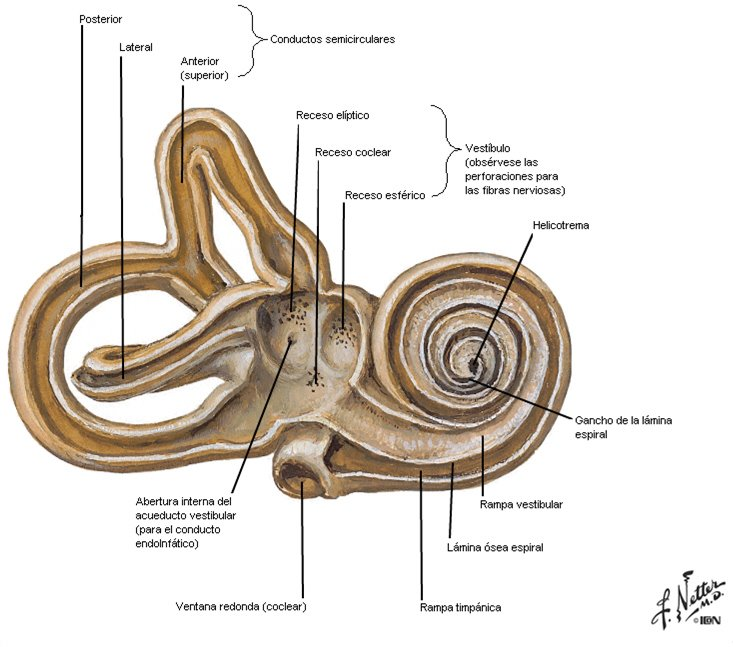
\includegraphics[scale=.5]{OInterno.jpg}
		\caption{Estructura del oído interno}
	\end{figure}
	
	Destacar que cada zona de la membrana basilar (Figura 12) es sensible a un rango de frecuencias concreto. Este hecho está relacionado con la forma en la que percibimos las diferentes frecuencias.
	
		\begin{figure}
			\centering
				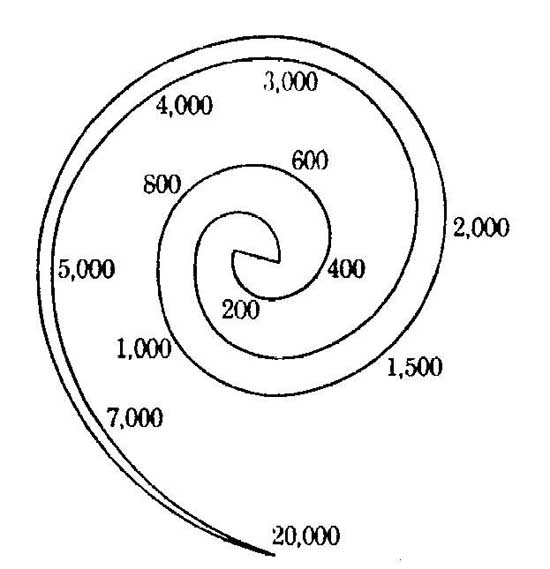
\includegraphics[height=50mm, width = 60mm]{RespFreqMemBasilar.jpg}
				\caption{Distribución de las zonas sensibles por frecuencias a lo largo de la membrana basilar}
		\end{figure}
		
	\subsection{Batidos}
	
	Antes de hablar de los batidos hablaremos del caso más simple de interacción entre dos ondas, cuando estas tienen la misma frecuencia, la \emph{Interferencia}.
	
	Cuando dos ondas son emitidas a la vez, si estas tienen la misma frecuencia, el sonido producido se corresponde con el de una única onda de la misma frecuencia, pero dependiendo de la relación entre las fases de las ondas involucradas la altura de la onda "percibida" puede ser mayor (\emph{interferencia constructiva}, misma fase) o menor (\emph{interferencia destructiva}, distinta fase) que la altura de las ondas originales.
	
	Remarcar que los sistemas de cancelación de ruido, como los cascos utilizados en fábricas, a groso modo se basan en el principio de la interferencia destructiva\cite{Set}, reciben la onda (en este caso no será una única onda) a cancelar, la analizan y emiten otra con la misma frecuencia y de fase la mitad del periodo (contraponiendo así el máximo de la onda original con el mínimo de la nueva onda).
	
	Cuando las frecuencias de las dos ondas implicadas tienen distinta frecuencia, es cuándo se producen los \emph{Batidos}.
	
	La forma más sencilla de pensar en el fenómeno es pensar que ambas ondas tienen la misma frecuencia y que, sin embargo, la fase entre ellas cambia poco a poco. Así, cuando las fases estén alineadas, se producirá la interferencia constructiva y, cuando no, destructiva.
	
	Usando trigonometría, es posible demostrar lo siguiente:
	
	$$
	  \hbox{\textnormal{batidos por segundo}} = | \left(\textnormal{freq. primera onda} \right) - \left( \textnormal{freq. segunda onda }\right) |
    $$
    
	\subsection{Formación de escalas}

	Como ya ha sido comentado antes, se atribuye a Pitágoras el descubrimiento de la particular consonancia del intervalo de quinta, la relación de $3:2$ entre las frecuencias de los sonidos que se encuentran a esta distancia. Basándose en esta relación y en la relación entre octavas ($2:1$), se construye una sucesión de notas particularmente ``consonantes'' (en la próxima sección intentaré precisar el significado de consonancia, por ahora quedémonos con la idea intuitiva y en absoluto precisa de que dos sonidos son consonantes si no suenan ``mal'') que es lo que hoy conocemos como \emph{escala pitagórica}.
	
	Una posible explicación al por qué la quinta es, después de la octava, el intervalo menos disonante entre dos notas se puede encontrar atendiendo a las posiciones relativas de sus parciales. Observaremos el espectro de una nota de frecuencia $f$ y el de su quinta, de frecuencia $\frac{3}{2}f$ (Figuras 13, 14, 15, 16):
		
    
    \begin{figure}[h]
        \centering
        \begin{tikzpicture} [xscale = 0.5, yscale = 1]
            \draw[thick, |->] (0,0) -- (22,0);
            \node[below] at (11,0) {frecuencia};
            \foreach \x in {1,2,3,4,5,6,7,8,9,10,11,12,13,14,15,16,17,18,19,20}
                \draw [red] (\x,0) -- (\x,1);
        \end{tikzpicture}
        \caption{Situación de los armónicos de la sinusoidal de frecuencia $f$}
    \end{figure}
    
    \begin{figure}[h]
        \centering
        \begin{tikzpicture} [xscale = 0.5, yscale = 1]
            \draw[thick, |->] (0,0) -- (22,0);
            \node[below] at (11,0) {frecuencia};
            \foreach \x in {1,2,3,4,5,6,7,8,9,10}
                \draw [blue] (\x*2,0) -- (\x*2,1);
        \end{tikzpicture}
        \caption{Situación de los armónicos de la sinusoidal de frecuencia $2f$}
    \end{figure}
    
    \begin{figure}[h]
        \centering
        \begin{tikzpicture} [xscale = 0.5, yscale = 1]
            \draw[thick, |->] (0,0) -- (22,0);
            \node[below] at (11,0) {frecuencia};
            \foreach \x in {1,2,3,4,5,6,7,8,9,10,11,12, 13}
                \draw (\x*1.5,0) -- (\x*1.5,1);
        \end{tikzpicture}
        \caption{Situación de los armónicos de la sinusoidal de frecuencia $\frac{3}{2} f$}
    \end{figure}
    
    \begin{figure}[h]
        \centering
        \begin{tikzpicture} [xscale = 0.5, yscale = 1]
            \draw[thick, |->] (0,0) -- (22,0);   % Ejes
            \node[below] at (11,0) {frecuencia};           
            \foreach \x in {1,2,3,4,5,6,7,8,9,10,11,12,13,14,15,16,17,18,19,20}    % frecuencia f
                \draw [red, fill] (\x,3) circle [radius=0.1];
            \foreach \t in {1,2,3,4,5,6,7,8,9,10,11,12,13,14,15,16,17,18,19,20}
                \draw [dashed] (\t,0) -- (\t,3);
            \foreach \y in {1,2,3,4,5,6,7,8,9,10}                                  % frecuencia 2f
                \draw [blue, fill] (\y*2,2) circle [radius=0.1];
            \foreach \z in {1,2,3,4,5,6,7,8,9,10,11,12, 13}
                \draw [black, fill] (\z*1.5,1) circle [radius=0.1];
            
        \end{tikzpicture}
        \caption{Comparación entre las posiciones de los armónicos de la fundamental (frecuencia $f$), la octava ($2f$) y la quinta($\frac{3}{2} f$)}
    \end{figure}
    
    
	Así podemos ver cómo las frecuencias de gran parte de mitad de las parciales de la quinta coinciden con las frecuencias parciales de la parcial y de su octava (frecuencia $2f$).
	
	El proceso que podemos seguir para reproducir la escala pitagórica es el siguiente:
		- Partimos de una nota, Do en este caso, a partir de la cual construiremos la escala.
		- Escogemos la siguiente nota menos disonante antes de llegar a la octava, Sol.
		- A partir de esta repetimos el proceso $5$ veces más, escogemos siempre la quinta de la última nota teniendo en cuenta dividir apropiadamente entre la razón de la octava para asegurarnos de que ninguna de estas notas se encuentra a una distancia mayor de la que abarca la octava a partir de la nota desde la que hemos empezado a construir la escala.
	   - La última de las siete notas, Fa, la escogeremos moviéndonos en la dirección contraria, escogeremos la nota de la cual es quinta Do.
	   
	 $$
		Fa \longleftarrow Do \longrightarrow Sol \longrightarrow Re \longrightarrow La \longrightarrow Mi \longrightarrow Si 
	 $$
	  
    Como observación notar que obtendríamos los mismos sonidos partiendo de la nota Fa y avanzando hacia frecuencias mayores $6$ veces en lugar de $5$.		
		
	Procedemos de la misma manera hasta obtener los 12 sonidos o notas que conforman la escala cromática: do, do\#, re, re\#, mi, fa, fa\#, sol, sol\#, la, la\#, si y de nuevo do (ordenados ya de mayor a menor altura).
		
	La escala atribuida a Pitágoras carece, en gran medida, de disonancia, sin embargo el proceso que hemos seguido para construirla no es perfecto, ya que no nos sirve para ordenar los $12$ sonidos de la escala cromática de manera que las distancias entre cada nota sean iguales, idealmente una quinta exacta.
		
	Observemos el proceso descrito sobre el llamado círculo de quintas (gráfico que ilustra el orden en el que se suceden las quintas a lo largo de los doce sonido de una escala cromática, Figura 17):
		
	\begin{figure}[h]
	    \centering
	    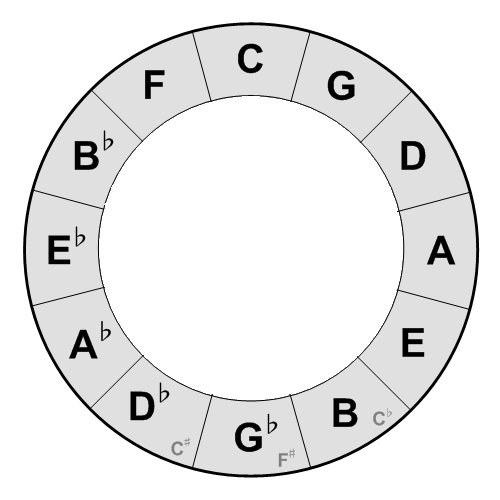
\includegraphics[scale = 0.5]{Quintas.jpg}
	    \caption{Representación del círculo de quintas}
	\end{figure}
	
	La distancia entre notas que difiere de la quinta en $23,46$ \textit{cents} \footnote{ Su expresión numérica, deducible del proceso ya explicado, es $ \left( \frac{3}{2} \right) ^{12} : 2^7 $. } (diferencia llamada \emph{coma pitagórica}) es la denominada \emph{quinta del lobo}. La posición de esta distancia puede variar dando lugar a diferentes escalas. También se obtienen escalas diferentes en función de la forma que elijamos de repartir esa diferencia entre más de un intervalo (perdiendo así el gran número de distancias de quinta perfecta que habíamos conseguido).
		
	Esto es así porque el sistema de afinación occidental es imposible de afinar, $12 \hbox{quintas} = \left( \frac{3}{2} \right)^{12} = 129.75$ mientras que la misma nota es la séptima octava de la original, es decir $2^7 = 128 $.
		
	%En cualquier caso la motivación para escoger entre el infinito rango de sonidos posibles unos concretos y no otros será la misma siempre que construimos una %escala, la disminución de la disonancia entre las notas que la conforman. Lamentablemente, como acabamos de ver, construir escalas donde únicamente estén %los intervalos que nos proporcionan la disonancia mínima no es posible.
		
	La escala Pitagórica de siete notas se ha convertido pues en una primera versión de la escala que se ha convertido en el corazón de la música occidental, la \emph{escala diatónica}. Las escalas diatónicas son las escalas de siete notas que contienen el máximo número de cuartas y quintas perfectas posibles ya que son construidas utilizando únicamente las razones ideales teóricas $3/2$ y $4/3$.
	
	\subsubsection{Temperamento igual}
	
	Para que las sucesivas notas de una escala suenen separadas de manera equidistante, cada intervalo deberá ser el mismo. Escribamos $s$ como este intervalo. Así, podemos escribir una escala con $12$ pasos igualmente espaciados como:
	$$
	1, s, s^2, s^3, s^4, s^5, s^6, s^7, s^8, s^9, s^{10}, s^{11}, s^{12}
	$$
	
	Si la escala se repite a distancia de octava, la nota final debe equivaler a una razón $2:1$. La ecuación $s^{12} = 2$ o equivalentemente $s = \sqrt[12]{2}$ tiene una única solución y tiene un valor aproximado de $1.05946$. Si tomamos las medidas en cents, la octava se correspondería con $1200$ cents y de esta forma, al estar ahora las notas situadas a la misma distancia las unas de las otras, cada intervalo de nuestra escala mide exactamente $100$ cents.
	
	Aunque dividir la octava en $12$ sonidos parece lo más natural en base a cómo se habían construido las escalas tradicionalmente, esto no tiene por qué ser así si, como lo hacemos, no partimos de las razones de quinta y cuarta sino de notas equi-espaciadas. Así podemos diseñar escalas con un número arbitrario $n$ de notas, sea $r = \sqrt[n]{2}$ tenemos:
	$$
	1, r, r^2, r^3, ....,r^{n-1}, r^{n}
	$$
	Esta escala contendrá $n$ pasos idénticos. El cálculo es más sencillo utilizando cents: la octava contiene $1200$ cents y por tanto, cada paso en la misma será de $1200/n$ cents.
	
	Las escalas de temperamento igual no tienen porqué estar basadas en la octava. Una escala con $n$ notas igualmente temperadas  en cada \emph{pseudo-octava} $p$ (con $p=2$ la octava) se basará en la razón $r = \sqrt[n]{p}$. Por ejemplo, una pseudo-octava $p = 2.1$ nos define un intervalo de $1284$ cents que, si dividimos en $12$ partes nos da una escala cuyas notas están separadas entre sí por $107$ cents. Otro ejemplo podría ser la pseudo-octava $p=2.0273$ de $1224$ cents, la cantidad justa que nos permite tener $12$ quintas perfectas (razón $3:2$).
	
	%% Gráfico temperamentos iguales:
	
	\begin{figure}[h]
	    \centering
	    \begin{tikzpicture}[xscale = .75, yscale= .50]
	        \foreach \y in {0,1,2,3,4,5,6,7,8,9,10,11,12} % Comparaciones con 12-tet
	            \draw (0,\y) -- (17,\y);
	        \foreach \v in {1,2,3,4,5,6,7,8,9,10,11}        % Marcadores a la izq.
	            \node[left] at (0,\v) {$\v00$};
	            \node[left] at (0,0) {$1/1$};
	            \node[left] at (0, 12) {$2/1 = 1200$};
	            \node[left] at (0, 13) {cents};
	        \foreach \u in {9,...,26}                       % Marcadores inferiores
	            \node[below] at (\u-9,0) {\u};
	            \node[below] at (8.5,-2) {Pasos por octava};
	        \foreach \w in {0,...,17}	            
	            \draw [black, fill] (\w,0) circle [radius=0.1];   % Marcadores a altura 0
	        \foreach \a in {1,...,9}
	        {
	            \draw [black, fill] (0,\a * 1.333) circle [radius=0.1];
	        }
%	        \foreach \w in {0,...,17} 
%	        {
	           % \foreach \a in {1.333,1.2,1.0909,1,0.923,0.8571,0.8,0.75,0.7058,0.666,0.6315,0.6,0.5714,0.5454,0.5217,0.5,0.48,0.4615} 
%	            \foreach \a in {9,...,26}
%	            {
%	                \foreach \n in {1,...,\a} 
%	                {
%	                    \draw [black, fill] (\w,\a * \n) circle [radius=0.1];
%	                 }
%	            }
%	       }
              \foreach \a in {1,...,10}
	        {
	            \draw [black, fill] (1,\a * 1.2) circle [radius=0.1];
	        }
	         \foreach \a in {1,...,11}
	        {
	            \draw [black, fill] (2,\a * 1.0909) circle [radius=0.1];
	        }
	          \foreach \a in {1,...,12}
	        {
	            \draw [black, fill] (3,\a * 1) circle [radius=0.1];
	        }
	          \foreach \a in {1,...,13}
	        {
	            \draw [black, fill] (4,\a * 0.923) circle [radius=0.1];
	        }
	          \foreach \a in {1,...,14}
	        {
	            \draw [black, fill] (5,\a * 0.8571) circle [radius=0.1];
	        }
	          \foreach \a in {1,...,15}
	        {
	            \draw [black, fill] (6,\a * 0.8) circle [radius=0.1];
	        }
	          \foreach \a in {1,...,16}
	        {
	            \draw [black, fill] (7,\a * 0.75) circle [radius=0.1];
	        }
	          \foreach \a in {1,...,17}
	        {
	            \draw [black, fill] (8,\a * 0.7058) circle [radius=0.1];
	        }
	          \foreach \a in {1,...,18}
	        {
	            \draw [black, fill] (9,\a * 0.666) circle [radius=0.1];
	        }  \foreach \a in {1,...,19}
	        {
	            \draw [black, fill] (10,\a * 0.6315) circle [radius=0.1];
	        }
	          \foreach \a in {1,...,20}
	        {
	            \draw [black, fill] (11,\a * 0.6) circle [radius=0.1];
	        }
	          \foreach \a in {1,...,21}
	        {
	            \draw [black, fill] (11,\a * 0.5714) circle [radius=0.1];
	        }
	          \foreach \a in {1,...,22}
	        {
	            \draw [black, fill] (12,\a * 0.5454) circle [radius=0.1];
	        }
	          \foreach \a in {1,...,23}
	        {
	            \draw [black, fill] (13,\a * 0.5217) circle [radius=0.1];
	        }
	          \foreach \a in {1,...,24}
	        {
	            \draw [black, fill] (14,\a * 0.5) circle [radius=0.1];
	        }
	          \foreach \a in {1,...,25}
	        {
	            \draw [black, fill] (15,\a * 0.48) circle [radius=0.1];
	        }
	          \foreach \a in {1,...,26}
	        {
	            \draw [black, fill] (16,\a * 0.4615) circle [radius=0.1];
	        }
	           \foreach \a in {1,...,27}
	        {
	            \draw [black, fill] (17,\a * 0.4444) circle [radius=0.1];
	        }
	    \end{tikzpicture}
	    
	    \caption{Afinaciones en los sistemas respecto a la afinación (líneas horizontales) 12-tet}
	\end{figure}
	
	
	
	\subsubsection{Entonación justa}
	
	Un problema que presenta la escala de temperamento igual con $12$ sonidos (12-tet de ahora en adelante) con $p = 2$ es que ninguno de los intervalos es puro. Por ejemplo, las quintas se encuentran a $700$ cents cuando deberían estar a $702$, la tercera menor que debería estar a $316$ cents se encuentra a $300$ y la tercera mayor que debería encontrarse a $386$ cents se encuentra a $400$. Hay más ejemplos, la sexta menor se encuentra $14$ cents por encima de lo que debiera y la sexta mayor $16$ cents por debajo de su posición natural. En el caso de la escala Pitagórica, estas diferencias pueden ser incluso mayores dándonos la tercera mayor a distancia de $408$ cents, una diferencia incluso mayor que la generada en la 12-tet.
	
	En escala mayor de entonación justa (JI) de 7 notas representada desde \textsl{Do} las terceras comienzan desde \textsl{Do, Do\#, Re, Re\#, Fa,Sol} y \textsl{Sol sos} y son todas quintas justas ($3:2$), las cinco nos darán acordes mayores perfectos. Por otro lado, también podemos crear esta escala pero partiendo de \textsl{Do, Re, Mi, Fa} y \textsl{La} y obtener así cinco acordes menores perfectos.
	
	Las escalas JI funcionan muy bien en una tonalidad especifica (y también en tonalidades cercanas a esta tonalidad en el círculo de quintas), sin embargo, lo hacen muy mal en otras. Pongamos como ejemplo un acorde de \textsl{Fa sos} mayor en una escala de \textsl{Do}, este tendrá desviada tanto su tercera mayor como su quinta (que se encontrará a una distancia de $722$ cents en lugar de los $700$ a los que debería estar). Frente a otros sistemas, cuando la JI se desvía se desvía por mucho. En este caso concreto sería imposible tocar adecuadamente una pieza que modulase entre las tonalidades implicadas.
	
	Otra crítica a este sistema es que, en la práctica, en una orquesta, para no estar limitados a unas pocas tonalidades, cada músico debería llevar $12$ instrumentos, uno por tonalidad (instrumentos ``tracidionales'', sin sistemas de entonación informatizada, como es el caso de  sintetizadores o de diversos sistemas para instrumentos electrificados que recogen la señal y la procesan antes de enviarla al amplificador).
 
 	La situación ideal sería poder afinar de manera dinámica y de forma automática, así al modular de un tono a otro, podríamos beneficiarnos de las bondades de este sistema sin sufrir sus problemáticas. Este es el objeto de las afinaciones adaptativas \cite{AT}. 
	
	\subsubsection{Tono medio y buen temperamento}
	
	En este caso nos quedaremos con $12$ sonidos por octava y nos las ingeniaremos para conseguir terceras perfectas y tríadas aceptables en las teclas centrales a expensas de conseguir peores terceras y tríadas en las teclas más remotas (pensando en un teclado, en general las teclas más remotas se corresponden con notas más alejadas del \textit{La central}, a $440$ Hz típicamente). Típicamente estas escalas se construyen a partir de un círculo de quintas similar al pitagórico, pero en el que ciertas quintas difieren de la relación $3:2$.

    %%%% TECLADO %%%%
    
%    \begin{figure}[h]
%        \centering
%        \begin{tikzpicture}[xscale = 0.5, yscale = 0.75]
%            \draw (7,12) -- (0,12) -- (0,0) -- (3,0);
%            %\draw [dashed] (3,0) -- (3,0.4) -- (7,0.4);
%            \draw (3,0) -- (3,0.4) -- (7,0.4);
%            \foreach \y in {1.5,7.5}
%                \draw (0,\y) -- (7,\y);
%            \foreach \y in {3,4.5,6,9,10.5}
%                \draw (0,\y) -- (3,\y);
%            \draw (7,2.6) -- (3,2.6) -- (3,3.4) -- (7,3.4);
%            \draw (7,4.1) -- (3,4.1) -- (3,4.9) -- (7,4.9);
%           \draw (7,5.6) -- (3,5.6) -- (3,6.4) -- (7,6.4);
%           \draw (7,8.6) -- (3,8.6) -- (3,9.4) -- (7,9.4);
%           \draw (7,10.1) -- (3,10.1) -- (3,10.9) -- (7,10.9);
%            \node[above] at (1.5,12) {Razón};
%            \node[above] at (5,12) {Cents};
%            
%            \node[center] at (1.5,0.75) {DO};
%            \node[center] at (1.5,2.25) {SI};
%            \node[center] at (1.5,3.75) {LA};
%            \node[center] at (1.5,5.25) {SOL};
%            \node[center] at (1.5,6.75) {FA};
%            \node[center] at (1.5,8.25) {MI};
%            \node[center] at (1.5,9.75) {RE};
%            \node[center] at (1.5,11.25) {DO};
%            
%            \node[center] at (5,3) {LA\#};
%            \node[center] at (5,4.5) {SOL\#};
%            \node[center] at (5,6) {FA\#};
%            \node[center] at (5,9) {RE\#};
%            \node[center] at (5,10.5) {DO\#};
%        \end{tikzpicture}        
%        \caption{Teclado genérico, lo utilizaré a la hora de explicar las diferencias entre las posiciones de las notas para diferentes afinaciones}
%    \end{figure}
	
	\subsubsection{Escalas espectrales}
	
	Tanto las escalas Pitagóricas como la escala de Entonación Justa incorporan intervalos definidos mediante razones enteras. Estas proporciones son musicalmente significativas porque la estructura armónica de muchos instrumentos musicales causa que sus parciales se solapen, unas pequeñas desafinaciones podrían bastar para producir sensación de aspereza y provocar batidos. Otra manera de crear escales es aprovechándonos de la estructura de su serie armónica, esto es, basándonos directamente en qué lugar ocupan sus parciales.
	
	Tenemos varias posibilidades: utilizar los ocho tonos de la cuarta octava de la serie de parciales, utilizar los $16$ tonos de la quinta octava, utilizar los $32$ tonos de la sexta octava, y, en general, utilizar los $2^{n-1}$ tonos de la $n^{th}$ octava.
	
	Como las frecuencias de las  parciales están equiespaciadas, no pueden estarlo perceptivamente. Las alturas de los tonos en la serie armónica se acercan, no hay dos intervalos entre notas contiguas iguales. 
	
	Estas escalas, incluso más que las de entonación justa, tienden a estar restringidas a tonalidades particulares. Según nos alejamos del centro tonal, los intervalos que eran perfectos dejan de serlo, alejándose cada vez más de la distancia exacta, así, para tonalidades muy lejanas los intervalos estarán muy lejos de ser los correctos. 
	
	\subsubsection{Mejoras de la escala}
	
	Pitágoras defendía la idea de que la consonancia entre los intervalos estaba causada por ser las razones entre ellos  números enteros pequeños. Rameau consideraba naturales los intervalos al estar ``dictados'' por los armónicos de los sonidos musicales. Lou Harrison (compositor estadounidense) escribió en \textit{Premier} \cite{LS} que ``El intervalo es justo o no es intervalo''. Para Harry Partch (compositor e inventor de instrumentos musicales, también estadounidense) la escala 12-tet era una ``camisa de fuerza''. Desde estos puntos de vista, 12-tet es un sistema conveniente (permite tener teclados prácticos, que hacen sencillo modular entre tonos) pero a la vez, constituye una defectuosa aproximación a los intervalos justos
	
	Helmholtz afirmó que los cantantes naturales sin entrenamiento son capaces de alcanzar los intervalos justos, pero que los músicos acostumbrados a los teclados con 12-tet se han entrenado para aceptar estas aplicaciones como correctas. Esta era su opinión, no soportada por ningún dato, es más, ciertos estudios (\cite{CA} \cite{BW}) muestran que esta tendencia no existe.
	
	Prácticamente todos los tipos de música usan algún tipo de escala, algún conjunto de todos los posibles sonidos que son usados por compositores e intérpretes para construir melodías y armonías. Tenemos, llegados a este punto, que ser conscientes de que un mismo intervalo puede ser más o menos consonante dependiendo del timbre del instrumento con el que son generados los sonidos que lo conforman. El uso musical que tendrá una determinada escala depende en gran medida del instrumento en el que va a ser interpretada.
	
	La estructura que tenga la escala dependerá de muchas cosas, pero es solo una parte de la experiencia sonora. La otra, tan importante como la primera, es el tipo de sonidos que la conformarán.
	
	
\newpage	
\section{Consonancia y disonancia}

	\subsection{Disonancia}
	
	Tenemos la idea intuitiva de que es la disonancia muy clara, dos sonidos serán más disonantes cuánto más desagradable sean de escuchar juntos. 
	Sin embargo, a lo largo de la historia de la teoría musical , los términos consonancia y disonancia han amparado diferentes significados.
	
	\textbf{-} Desde la Grecia clásica hasta aproximadamente el siglo IX, el término hacía referencia exclusiva a las relaciones entre los diferentes tonos en un contexto melódico y su principal utilidad se daba en el desarrollo de escalas.
	
	\textbf{-} En los comienzos de la polifonía, aproximadamente entre los años $900$ y $1300$, los términos hacían referencia a la calidad del sonido producido al emitirse dos notas simultáneamente. En este periodo solamente seis intervalos eran considerados consonantes: la octava ($2:1$), la quinta ($3:2$), la cuarta ($4:3$), un intervalo de octava seguido de uno de quinta ($3:1$),  un intervalo de octava más uno de cuarta ($8:3$) y dos intervalos de octava consecutivos ($4:1$).
	
	\textbf{-} Entre los años $1300$ y $1700$ la noción de consonancia, además de incluir como intervalos consonantes terceras y sextas, se considera una nota consonante en función del contexto en el que esta es agregada, pudiendo así una misma nota ser o no consonante. La consonancia por tanto no es una característica intrínseca de un sonido.
	
	\textbf{-} En el siglo XVIII Rameau (compositor, intérprete y teórico musical francés) introduce el concepto de raíz fundamental, así una nota será consonante o no dependiendo de su relación con la nota raíz fundamental. A esta noción de consonancia la llamaremos \emph{consonancia funcional}. Rameu escribió:
	
	\begin{center}
    	``Los sonidos en general, de los intervalos y acordes, descansan finalmente en una fuente única y fundamental que es representada por la cuerda  invivisible...''.
	\end{center}
		
	La noción de nota raíz fundamental no solo implica la noción básica de ser la nota más grave en un acorde, sino que también contempla la noción dinámica de consistir en una sucesión de estas notas. La disonancia ocurre cuando la música se ha alejado de su raíz, lo que causa una sensación de expectación ante volver a la raíz. La disonancia funcional no está relacionada directamente con el movimiento armónico.
	
	En el siglo XVII, fue descubierto que una nota simple de un instrumento convencional de viento a cuerda tiene como parciales múltiplos enteros de su frecuencia. Rameau también se percató de que esta podía ser una posible explicación a la consonancia entre intervalos, sin embargo, Sorge fue el primero en considerar la espereza causada por la cercanía de las parciales como una posible causa de la disonancia.
	
	La noción de que la disonancia causa movimiento sigue viva en la música moderna. Por ejemplo, Walter Piston escribió:
	
	\begin{center}
    	`` Un intervalo consonante es aquel que suena estable y completo, mientras que la característica de un intervalo disonante es la inquietud y su necesidad de ser resuelto a un intervalo consonante... la música sin intervalos disonantes es a menudo negativa y sin vida, ya que es el intervalo disonante el que proporciona la sensación de movimiento y energía rítmica... No es posible enfatizar demasiado que la cualidad fundamental de la disonancia es la de proporcionar una sensación de movimiento, y no como se asume a veces de manera errónea, su grado de disgusto al oído''.       %pg 79 Sethares
	\end{center}
	
	\textbf{-} En el siglo XIX Helmholtz retomó la idea de entender la consonancia como la calidad del sonido resultante de la fusión de dos notas sonando de manera simultánea. Llamaremos a esta noción de consonancia \emph{consonancia psico-acústica}. La principal novedad que aportó es que introdujo una explicación física al fenómeno de la consonancia: la teoría de los batidos. La explicación de Helmholz fue puesta en firme en el siglo XX con la idea de la franja crítica de la membrana basal, especialmente con el trabajo de Plomp y Levelt (1965).
	
	El descubrimiento de la relación entre la frecuencia y el tono de un sonido ocurrió entre los siglos XVI y XVII y vino de la mano de, independientemente, Galileo Galilei (astrónomo, filósofo, ingeniero, matemático y físico italiano) y Mersenne (sacerdote, matemático y filósofo francés que estudió diversos campos de la teología, matemáticas y la teoría musical). La explicación para la disonancia de Galileo era que si la razón entre las frecuencias de los sonidos implicados es un número entero, entonces existe una periodicidad o regularidad en la onda total (onda suma), no presente con otras razones. Por ejemplo, las suma de una onda y una onda de razón $3:2$, es decir, una quinta justa:
	
	\begin{figure}[h]
		\centering	
		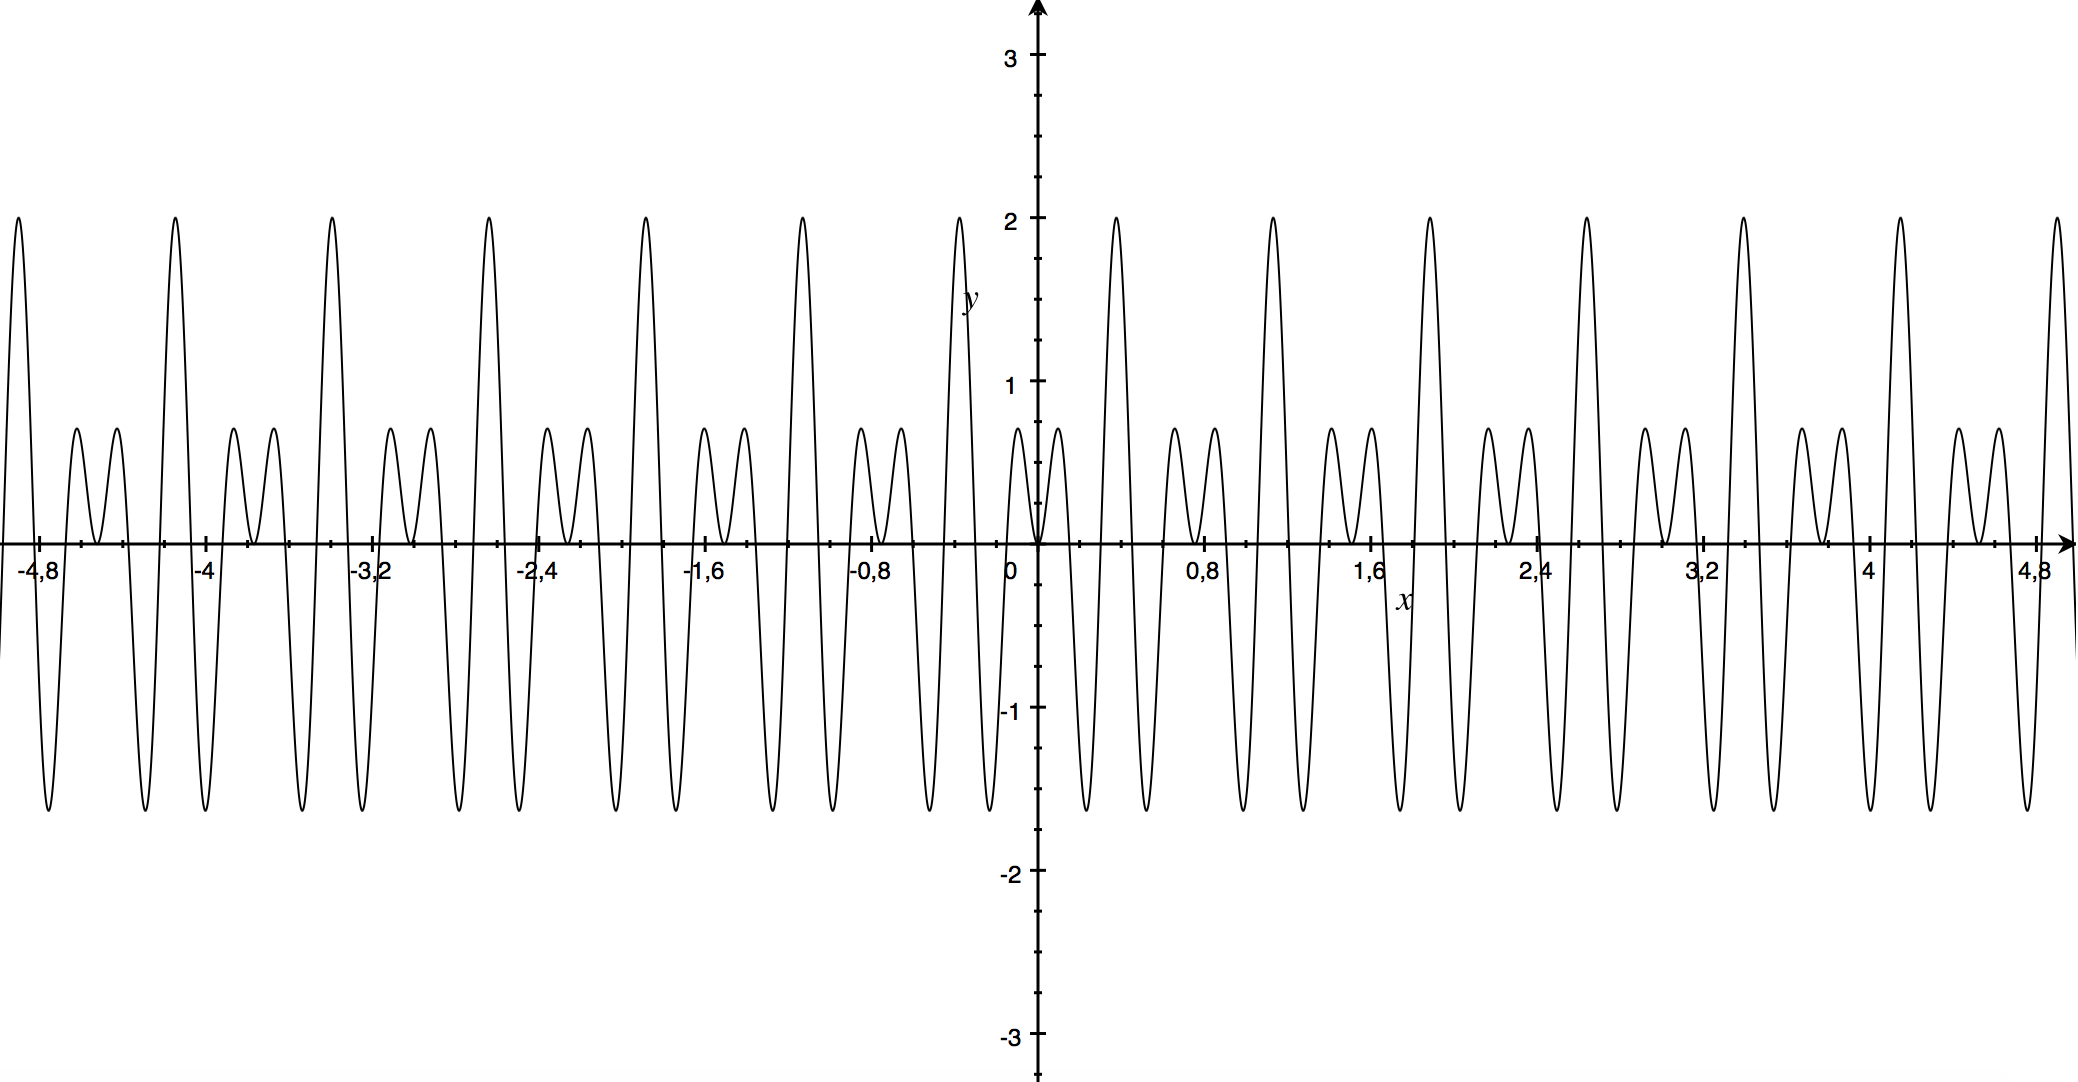
\includegraphics[scale=.35]{Quinta}         %CORRECTA
		\caption{Suma dos sonidos a distancia de quinta justa($3:2$)}
	\end{figure}
	
		\begin{figure}[h]
		\centering	
		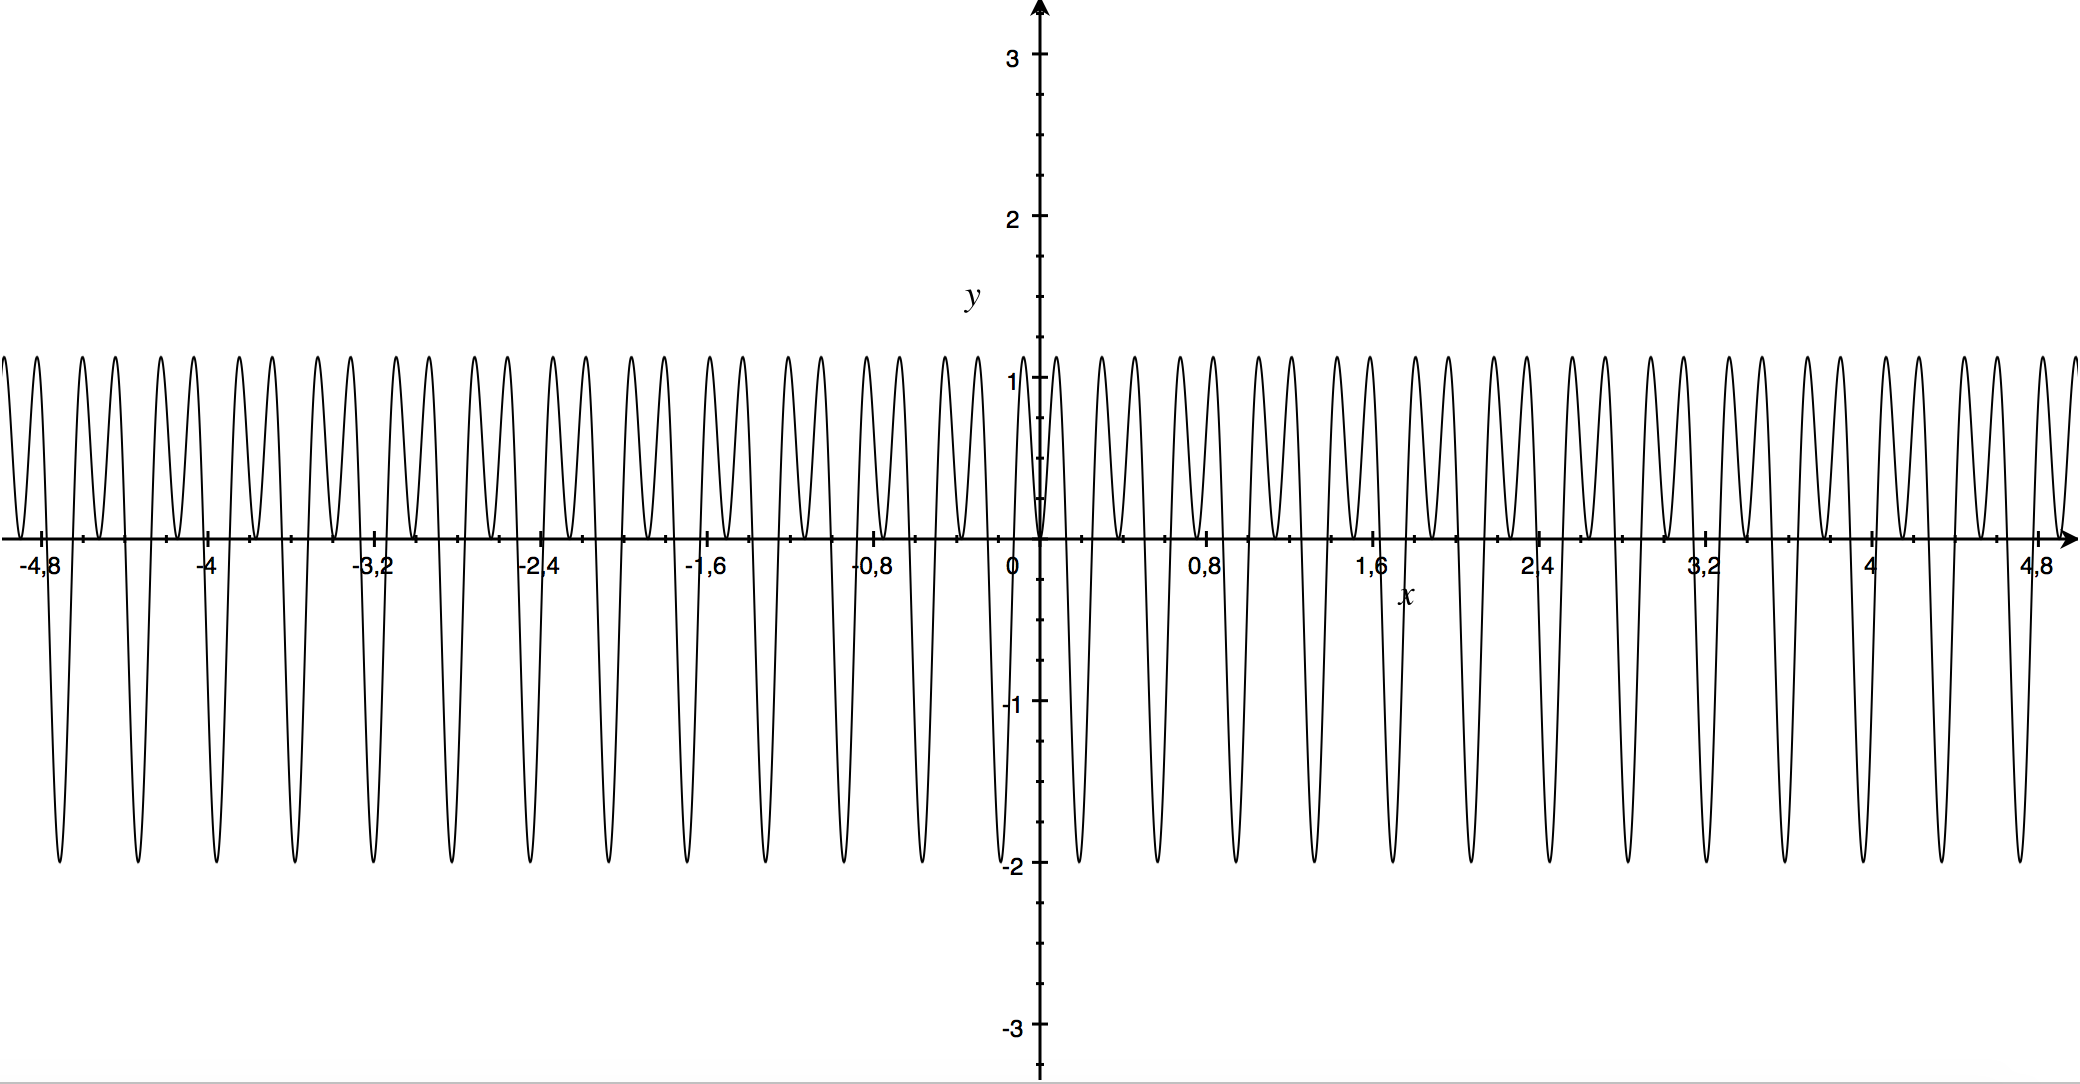
\includegraphics[scale=.35]{Octava}
		\caption{Suma dos sonidos a distancia de octava ($2:1$)}
	\end{figure}
	
	\begin{figure}[h]
		\centering	
		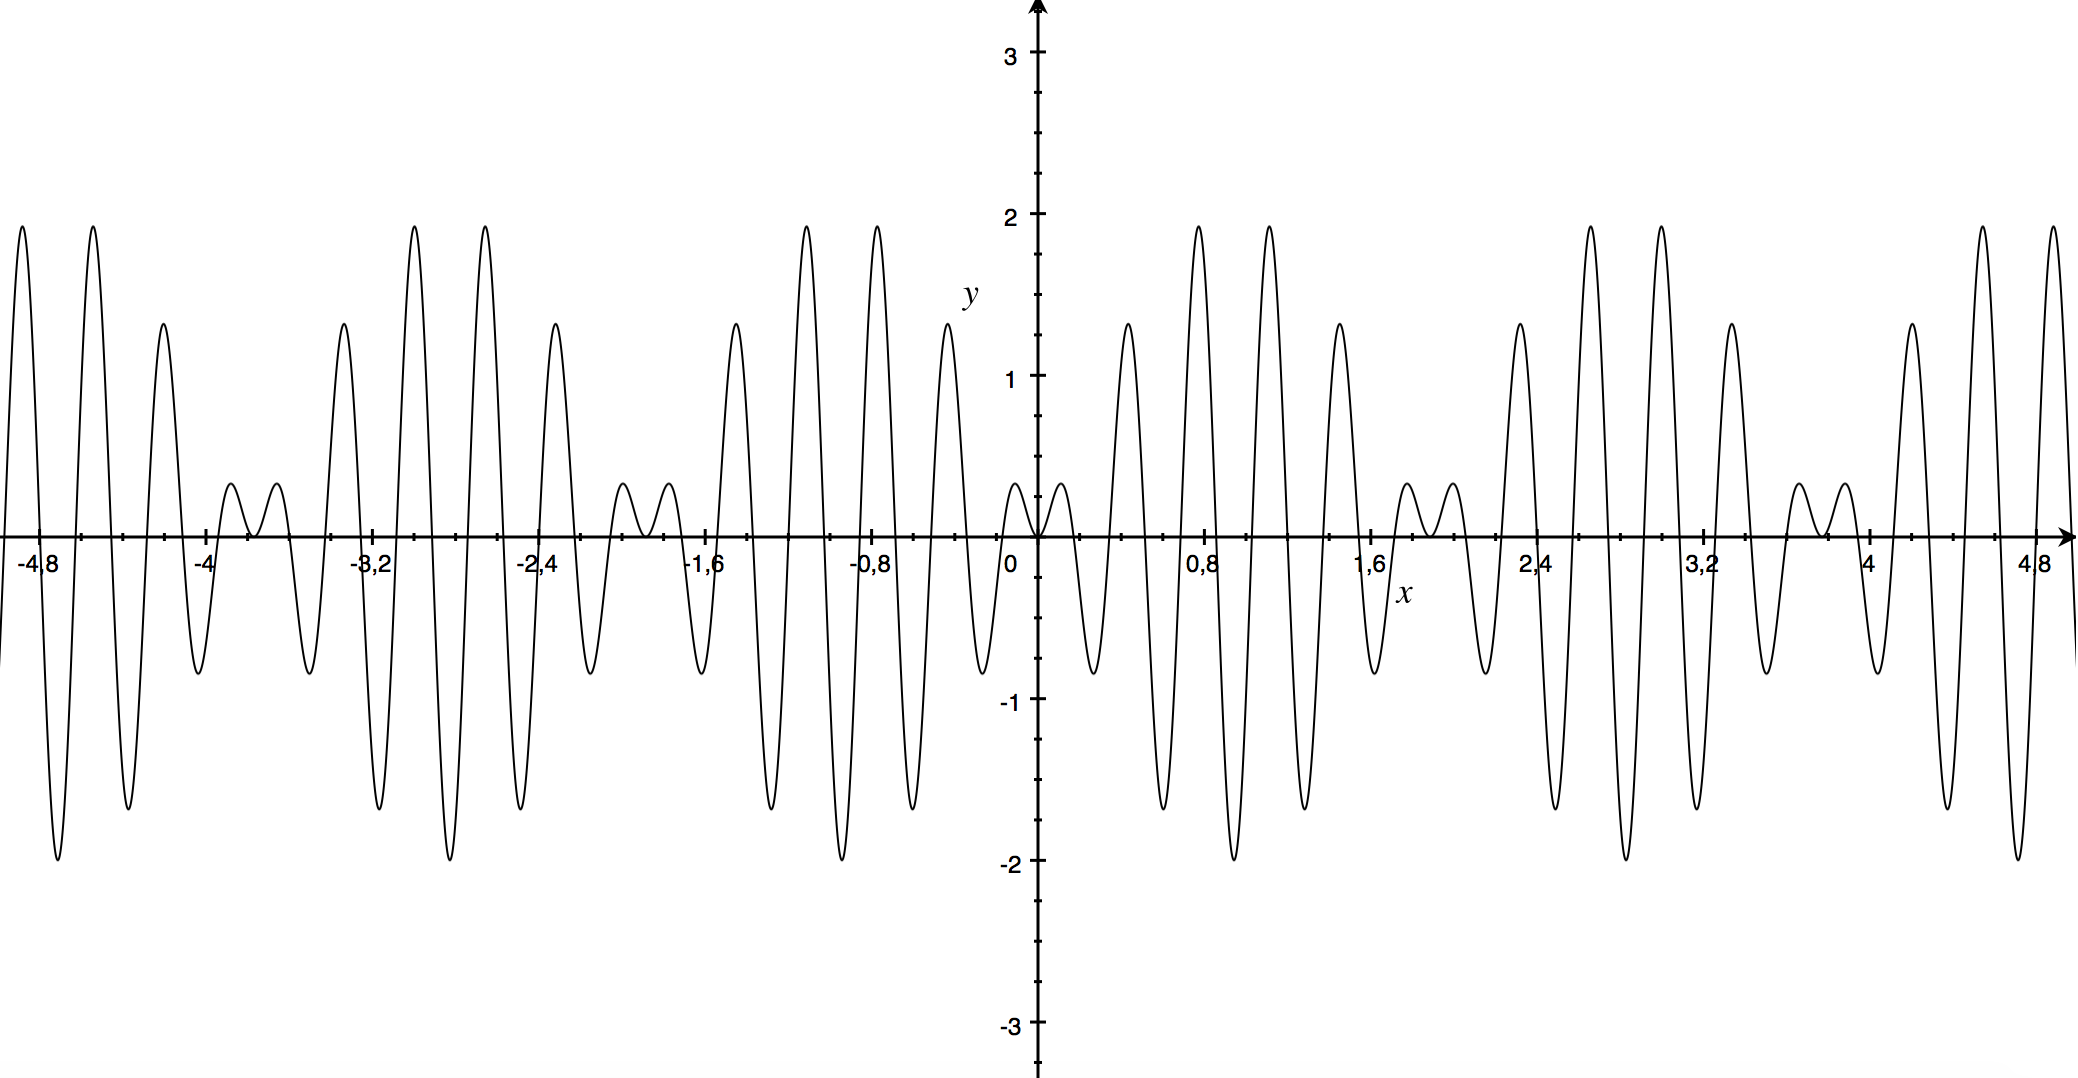
\includegraphics[scale=.35]{TerceraMenor}
		\caption{Suma dos sonidos a distancia de una tercera menor ($6:5$)}
	\end{figure}
	
	\begin{figure}[h]
		\centering	
		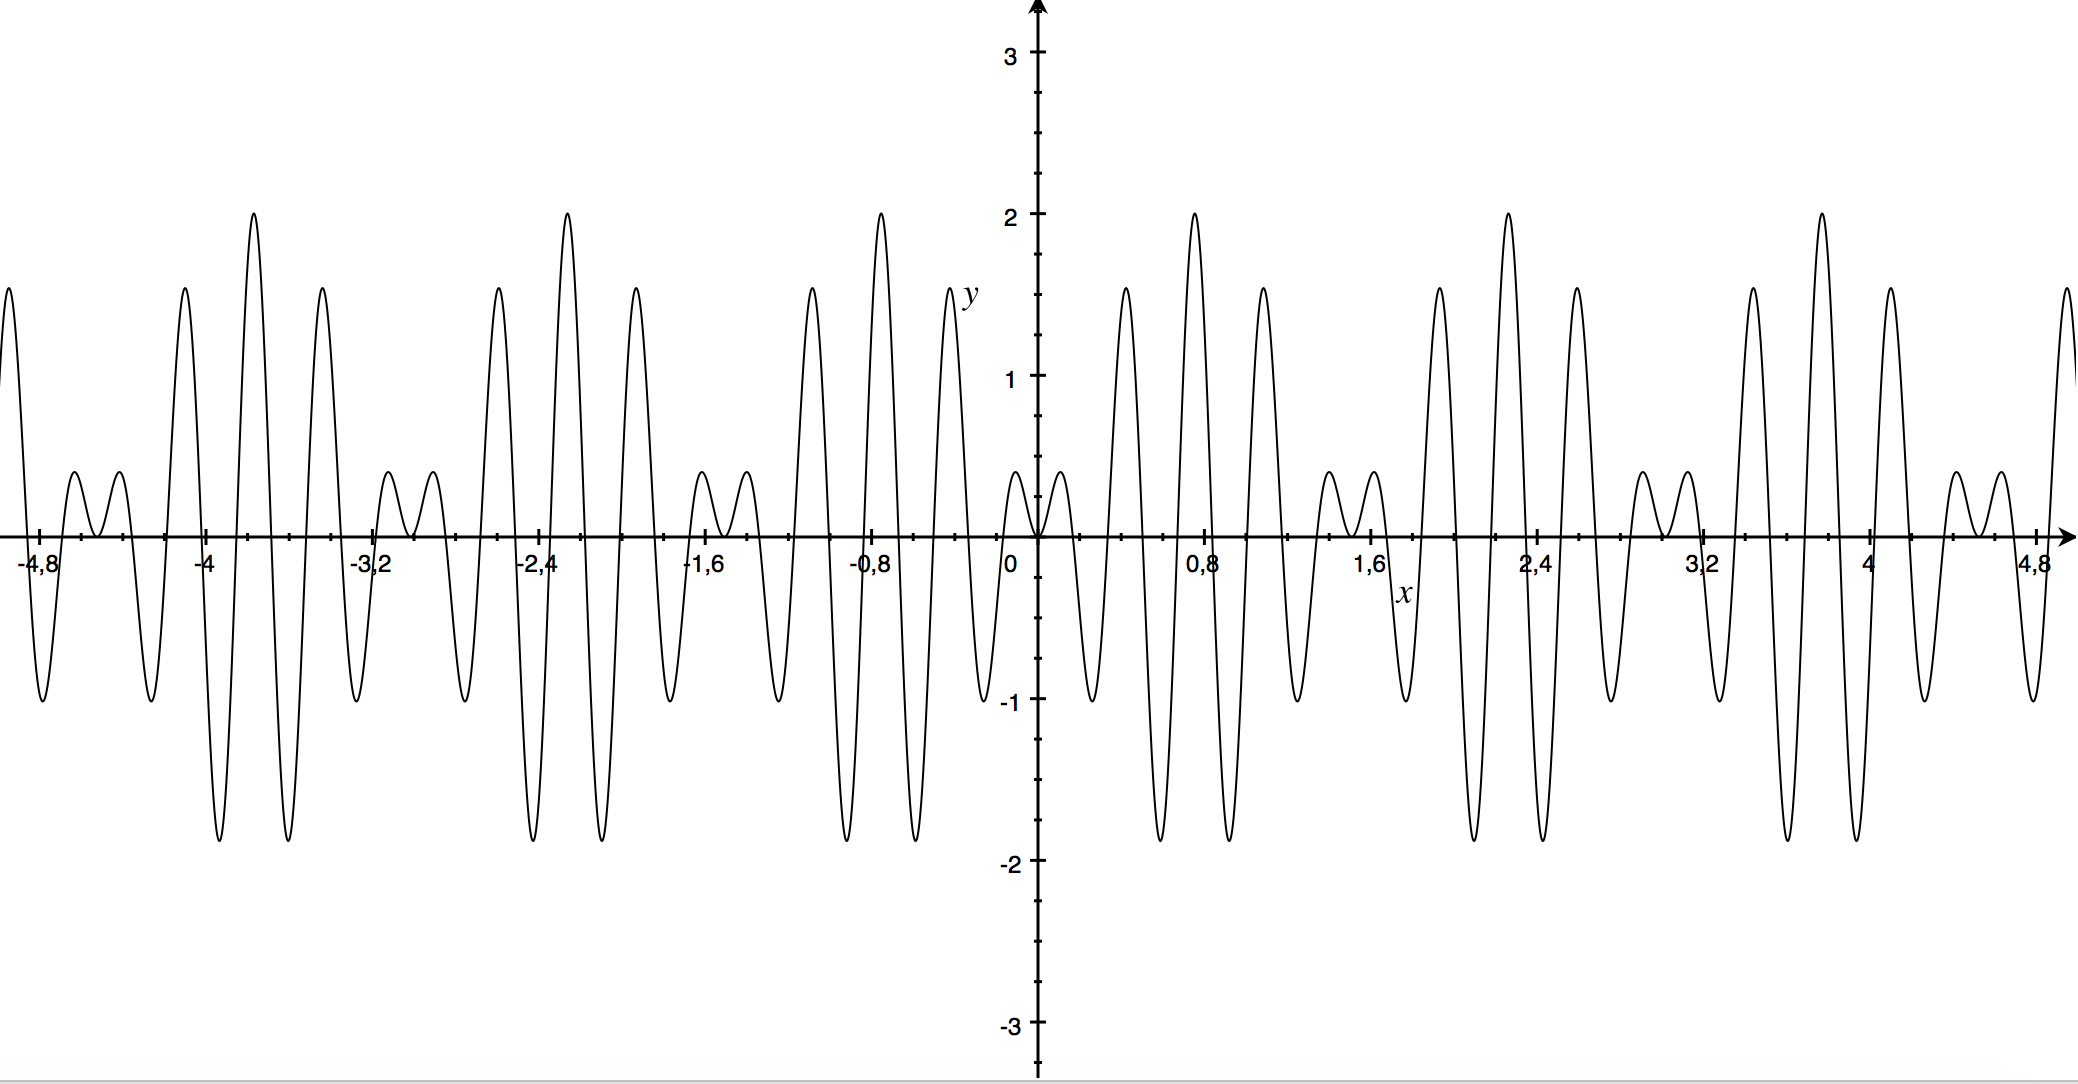
\includegraphics[scale=.35]{TerceraMayor}
		\caption{Suma dos sonidos a distancia de una tercera mayor justa ($5:4$)}
	\end{figure}
	
	\begin{figure}[h]
		\centering	
		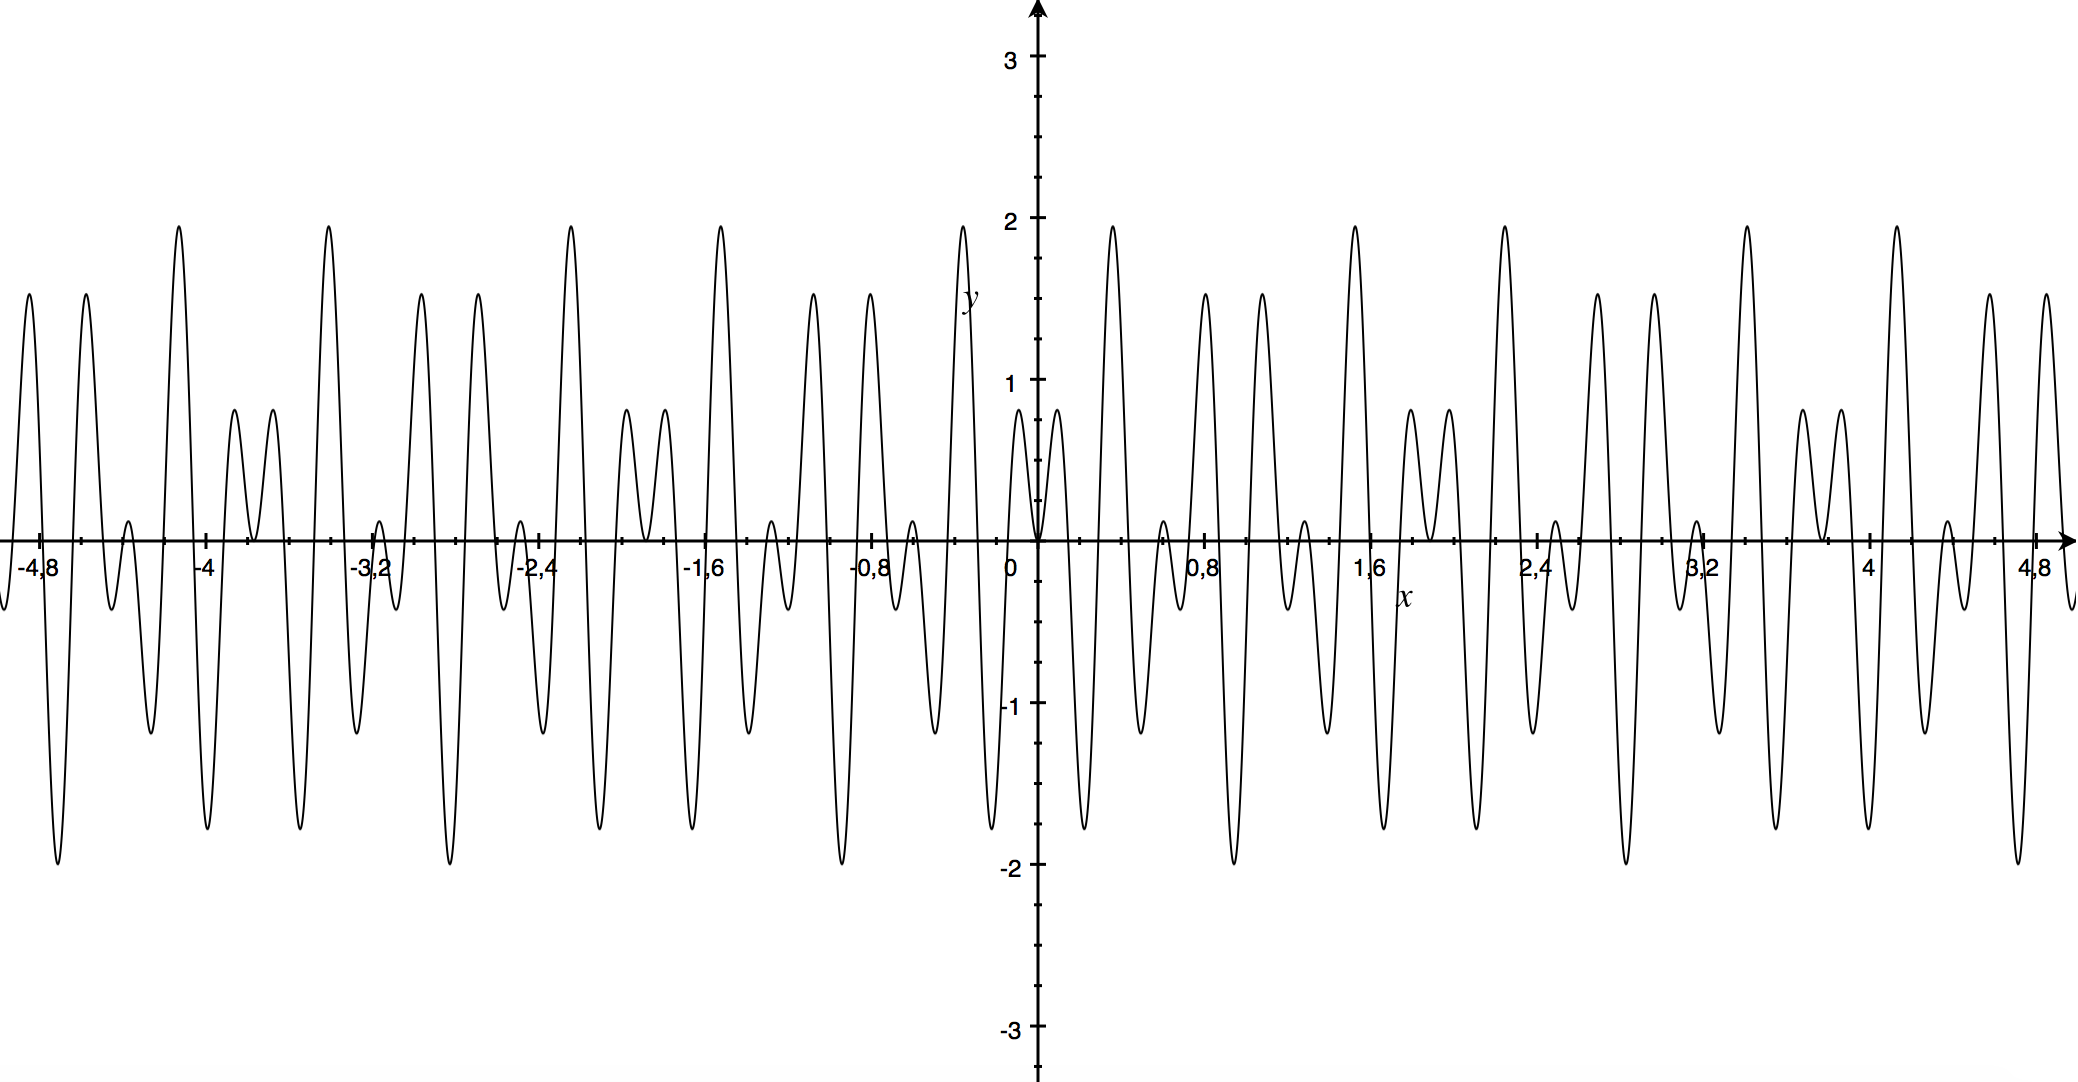
\includegraphics[scale=.35]{SextaMenor}
		\caption{Suma dos sonidos a distancia de una sexta menor justa($8:5$)}
	\end{figure}
	
	\begin{figure}[h]
		\centering	
		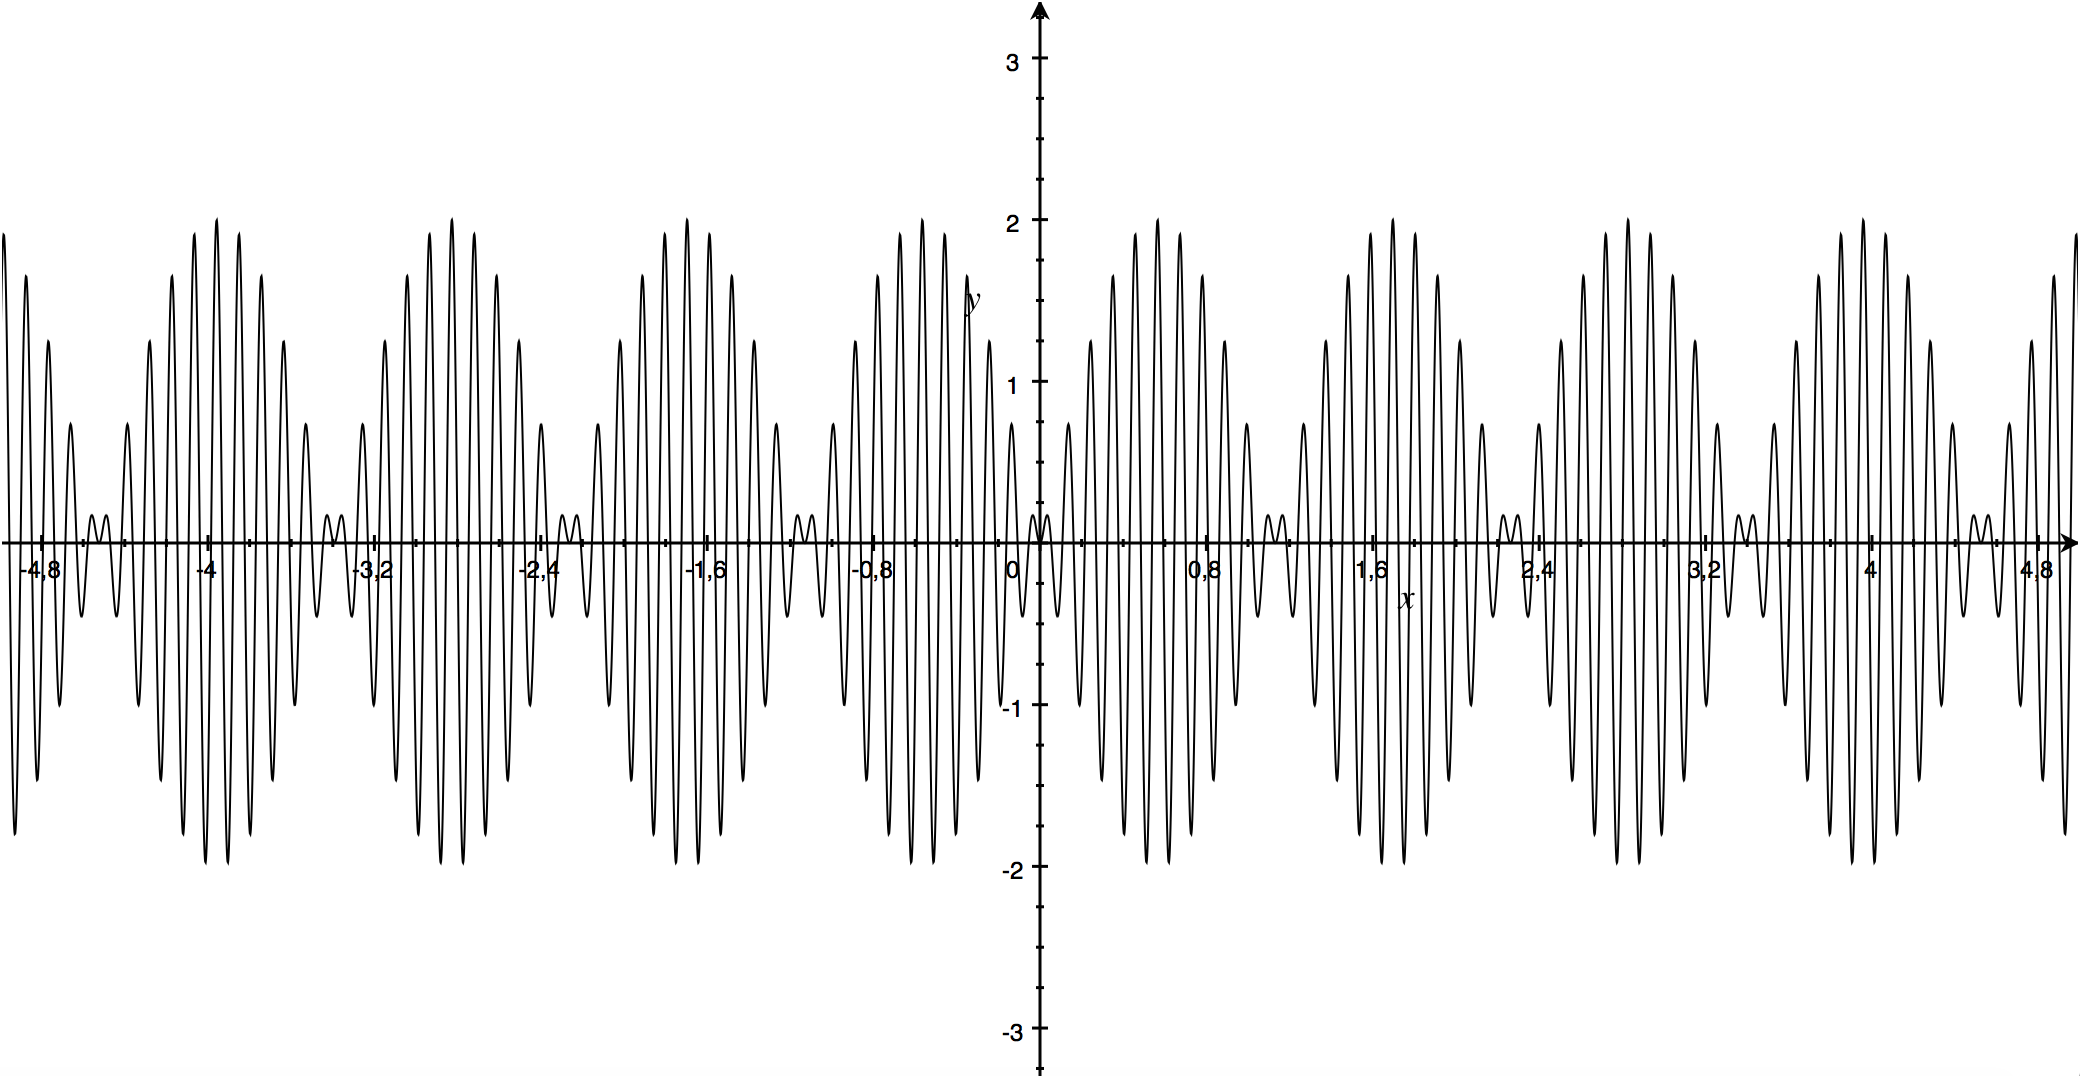
\includegraphics[scale=.35]{SextaMayor2}
		\caption{Suma dos sonidos a distancia de una sexta mayor justa($5:3$)}
	\end{figure}
	
	
	Uno de los problemas que atañen a esta explicación es el de ser un argumento circular, es decir, las notas son consonantes porque nuestro oído las interpreta como consonantes.
	
	
	\subsection{Teoría disonancia}
	
	Desde el momento en que hay maneras de entender la consonancia, para cada una habrá teoría diferente detrás que la explica. En la siguiente sección desarrollaré una de ellas, la teoría de Helmholtz, en la siguiente, la que desarrollaron R. Plomp y W.J.M. Levelt sobre los trabajos de este. Ahora, presentaré aquí otras posibles teorías.
	
	\subsubsection{Razones enteras}
		
	La explicación más simple: encontramos los intervalos basados en razones enteras y pequeñas más agradables porque los preferimos. Este argumento, a pesar de ser circular, fue la explicación preferida por Pitágoras. Galileo escribió:
	
	\begin{center}
	    ``Las consonancias agradables son aquellos pares de tonos que golpean el oído con una cierta regularidad; esta consiste en el hecho de que los pulsos entregados por los dos tonos, en el mismo intervalos de tiempo, deben ser mesurables en número, entonces no mantienen el tímpano en perpetuo tormento, doblándose en dos direcciones diferentes para nunca producir impulsos discordantes''. %pg81
	\end{center}
	
	Un enfoque más moderno de la misma idea (minimizar el ``perpetuo tormento'') nos lleva a ver la consonancia en términos del periodo de la onda resultante de la suma de dos tonos diferentes: cuanto más pequeño sea el periodo, mayor consonante será el intervalo. Entonces, una onda sumada con otra de periodo $3/2$ es altamente consonante porque la resultante se repite cada $6$ periodos y otro sumada a la primera pero con una frecuencia de razón $301/200$ es disonante porque la onda no se repite hasta $60200$ periodos.
	
	En esencia el cambio en el argumento consiste en sustituir ``al oído le gustan las razones pequeñas'' por ``al oído le gustan las ondas de periodo corto''.	
	
	\subsubsection{Fusión}
	
	La fusión de dos sonidos simultáneos es directamente proporcional a la capacidad de estos de ser percibidos como una unidad. Esta fusión está directamente relacionada con el alineamiento de las parciales del que ya hemos hablado con anterioridad. El oído no es capaz de discernir qué parciales pertenecen a qué sonidos si estos suenan simultáneamente así, cuando las parciales coinciden, los sonidos acaban por perder su carácter individual y se ``fusionan'' entre ellos.  C. Stumpf (filósofo y psicólogo alemán) determinó que el grado de fusión de los intervalos y que de la misma manera, la consonancia depende del grado de fusión entre los sonidos considerados.
	
	\subsubsection{Tono virtual}
	
	Rameau centraba el foco en las propiedades físicas de las ondas. Ahora cambiaremos el punto de vista y nos centraremos en la percepción del oyente. Terhardt enfatizó con sus teorías el rol que juega el aprendizaje del lenguaje en la percepción de los intervalos. Diferentes experiencias de aprendizaje guían hacia diferentes maneras de interpretar los intervalos y las escalas en términos de la consonancia o disonancia de los mismos.
	
	Uno de los principales elementos de la teoría del tono virtual es que el sistema auditivo trata de localizar el armónico templado más cercano confrontándolo con una colección de parciales. Esto puede ser ambiguo si el sonido de desvía de la armonía. La idea de entropía armónica cuantifica esta desviación midiendo la tonalidad de un intervalo basándose en la incertidumbre envuelta en interpretar el intervalo en términos de razones simples enteras.
	
	\subsubsection{Tonos diferentes}
	
	En ocasiones cuando dos ondas de diferentes frecuencias suenan juntas, es posible escuchar una tercera onda con una frecuencia igual a la diferencia de frecuencia entre las otras dos. Por ejemplo, cuando dos ondas, una de $f = 450$ Hz y otra de $g =570$ suenan al mismo tiempo, es posible a veces escuchar una tercera onda de frecuencia $ | f - g | = 120$ Hz. Sobre estos \emph{tonos diferentes} Roederer (es un profesor de física de la Universidad de Alaska Fairbanks, siendo sus campos de investigación la física del espacio y la psico-acústica entre otros)  escribió: ``estos (estos tonos) tienden a volverse más significativos cuando los tonos que les dan lugar son emitidos a intensidades altas''. Bajo ciertas condiciones estos tonos diferentes también son audibles en otras frecuencias, como por ejemplo $2f-g$,  o $3g-2f$\footnote{En general, estos tonos diferentes de mayor orden se dan a frecuencias $(n+1)g - nf$ donde $n$ es un número entero}. Cuando la razón entre $f$ y $g$ es un número entero, existen pocos tonos diferentes entre los armónicos de $f$ y $g$, por ejemplo, si las notas están a distancia de una octava (esto es razón $2:1$), los tonos diferentes se producen a frecuencias que coinciden con las de los armónicos. Sin embargo, cuando la complejidad en la relación entre los sonidos implicados crece, el número de tonos diferentes se incrementa. Posteriormente fue propuesto que la disonancia es directamente proporcional al número de tonos diferentes, ocurriendo la consonancia cuando hay pocos de estos tonos.
	
	Podría parecer que este fenómeno y el fenómeno de los batidos son el mismo porque ocurren ambos a frecuencia $f-g$, pero no es así. Recordemos que la esencia del fenómeno de los batidos es la fluctuación en la amplitud de la onda suma. Hall probó, mediante una seria de tests \cite{H}, que ambos fenómenos son distinguibles. Este fenómeno el y el del tono virtual tampoco son lo mismo.
	
	
	\subsection{Helmholtz}
	
	No fue hasta el siglo XIX cuando Helmholtz (médico y físico alemán) acertó a explicar su idea de disonancia basándose en el estudio de la estructura del sistema auditivo humano. Su idea fue que para diferencias pequeñas entre las frecuencias de las parciales, los batidos serán perceptibles pero que sin embargo, para diferencias mayores, estos son percibidos como aspereza. Él afirmó, que para alcanzar el máximo de aspereza, la diferencia entre las dos frecuencias debería ser de entre $30$ y $40$ Hz independientemente de las frecuencias individuales. Para frecuencias mayores, la sensación de aspereza desaparece en pro de la consonancia. Basándose en este argumento dedujo que el motivo por el que la octava es el intervalo más consonante es porque las parciales se alinean, es decir, no hay diferencia entre las frecuencias de esta y, por tanto, no se producen los batidos.
	
	Utilizaremos la siguiente identidad trigonométrica para analizar el fenómeno:
	$$ \sin(x) + \sin (y) = 2 \sin \left( \frac{x - y}{2} \right) \sin \left( \frac{x + y}{2} \right)$$
	
	Supongamos primero que ambas ondas tienen una misma frecuencia, $\omega$, y una diferencia constante de fase, $\phi$. Utilizando la anterior igualdad podemos escribir la suma de ambas ondas como sigue:
	$$ \sin (\omega t) + \sin (\omega t + \phi) = 2 \sin \left(\frac{\phi}{2} \right) \sin \left( \omega t  + \frac{\phi}{2} \right) $$
	
	Esto es  una nueva onda de amplitud $2 \sin \left( \frac{\phi}{2} \right) $, frecuencia $ \omega $ y fase $ \frac{\phi}{2} $. Observemos que cuando la diferencia de fase se acerca a cero, la interferencia es constructiva y que al aumentar esta tendremos una interferencia destructiva.
	
	Cuando las frecuencias difieren en una cantidad $\Delta \omega $ la suma de ondas es:
	$$ \sin(\omega t) + \sin ((\omega + \Delta \omega)t) = 2 \cos \left( \frac{\Delta \omega}{2} t \right) \sin \left( \left( \omega + \frac{\Delta \omega}{2} \right) t \right) $$
	
	Cuando $\Delta \omega $ es pequeño, el término del coseno varía lentamente en comparación con el término del seno, y la señal resultante puede ser vista como una onda sinusoidal de frecuencia $ \omega + \Delta \omega $ con una lenta variación alrededor de frecuencia $\Delta \omega$ (Figuras 25, 26 y 27).
	
	\begin{figure}[h]
		\centering
		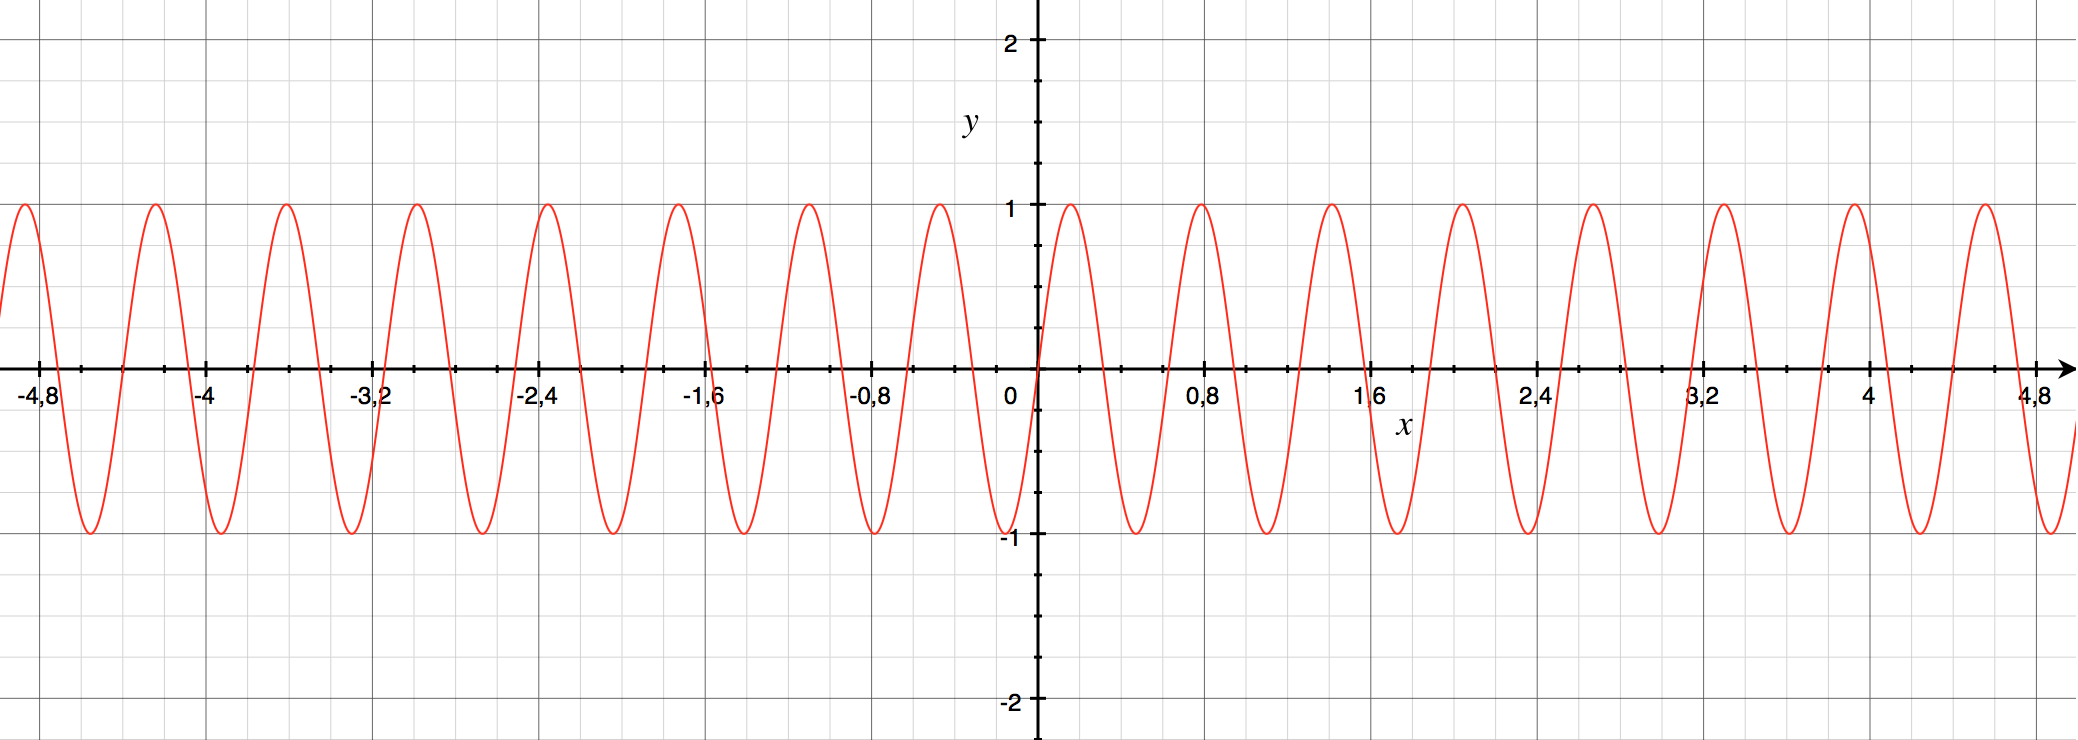
\includegraphics[scale=.4]{S1}
		\caption{$\sin(10 x)$}
	\end{figure}
	\begin{figure}[h]
		\centering
		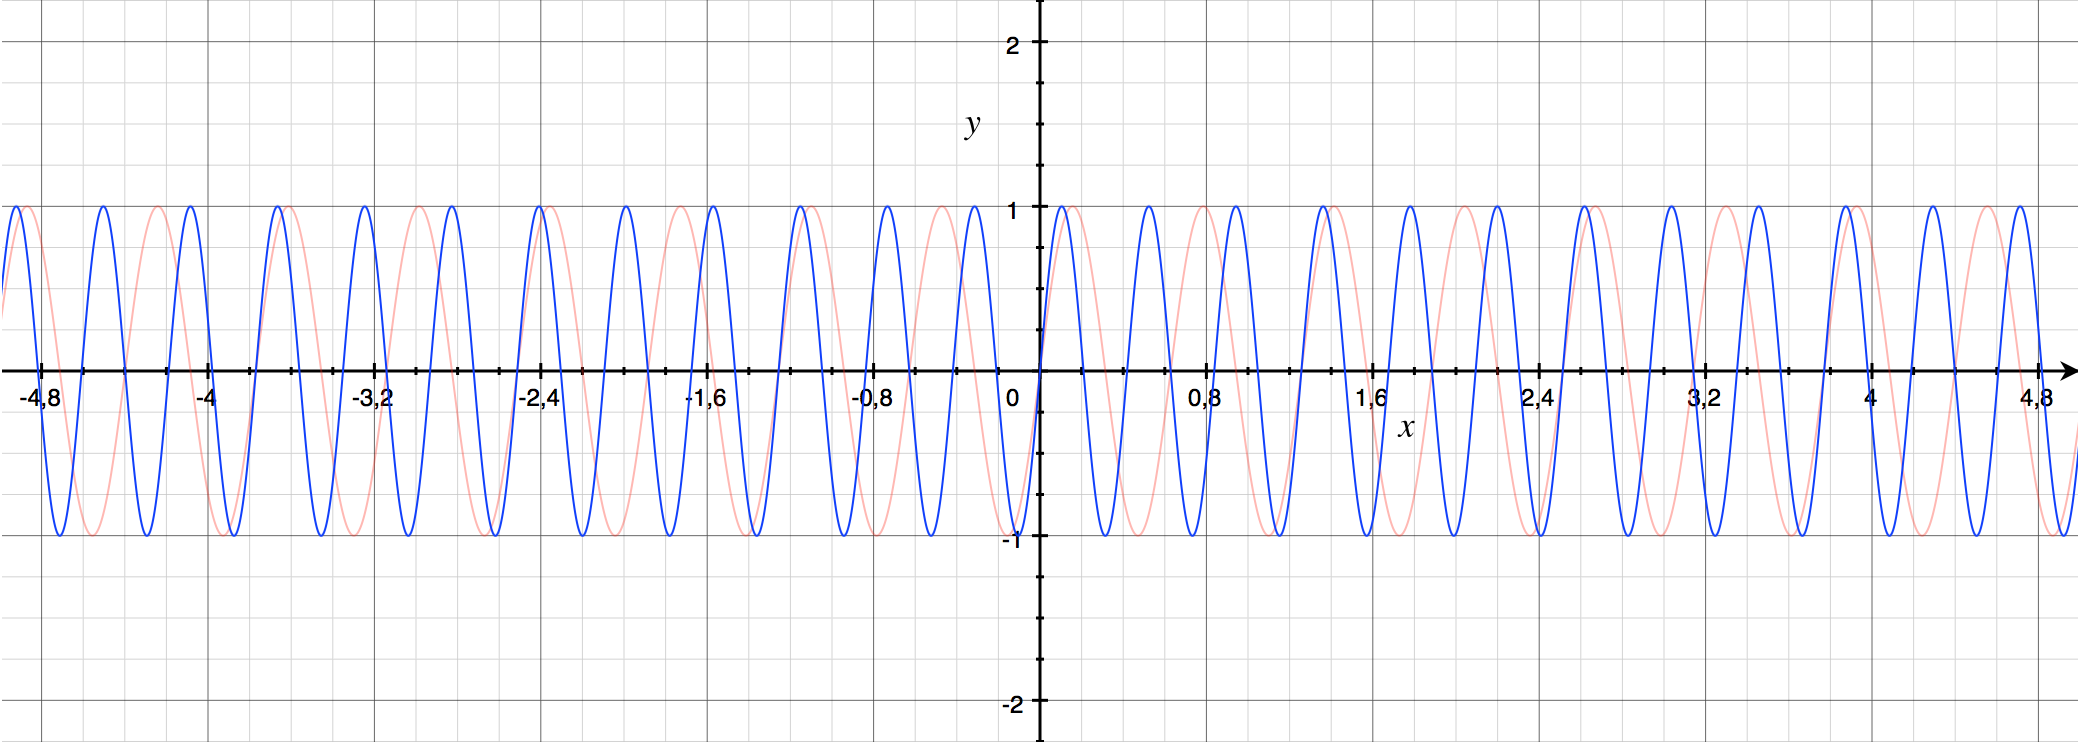
\includegraphics[scale=.4]{S2}
		\caption{$\sin(15 x)$}
	\end{figure}
	\begin{figure}[h!]
		\centering
		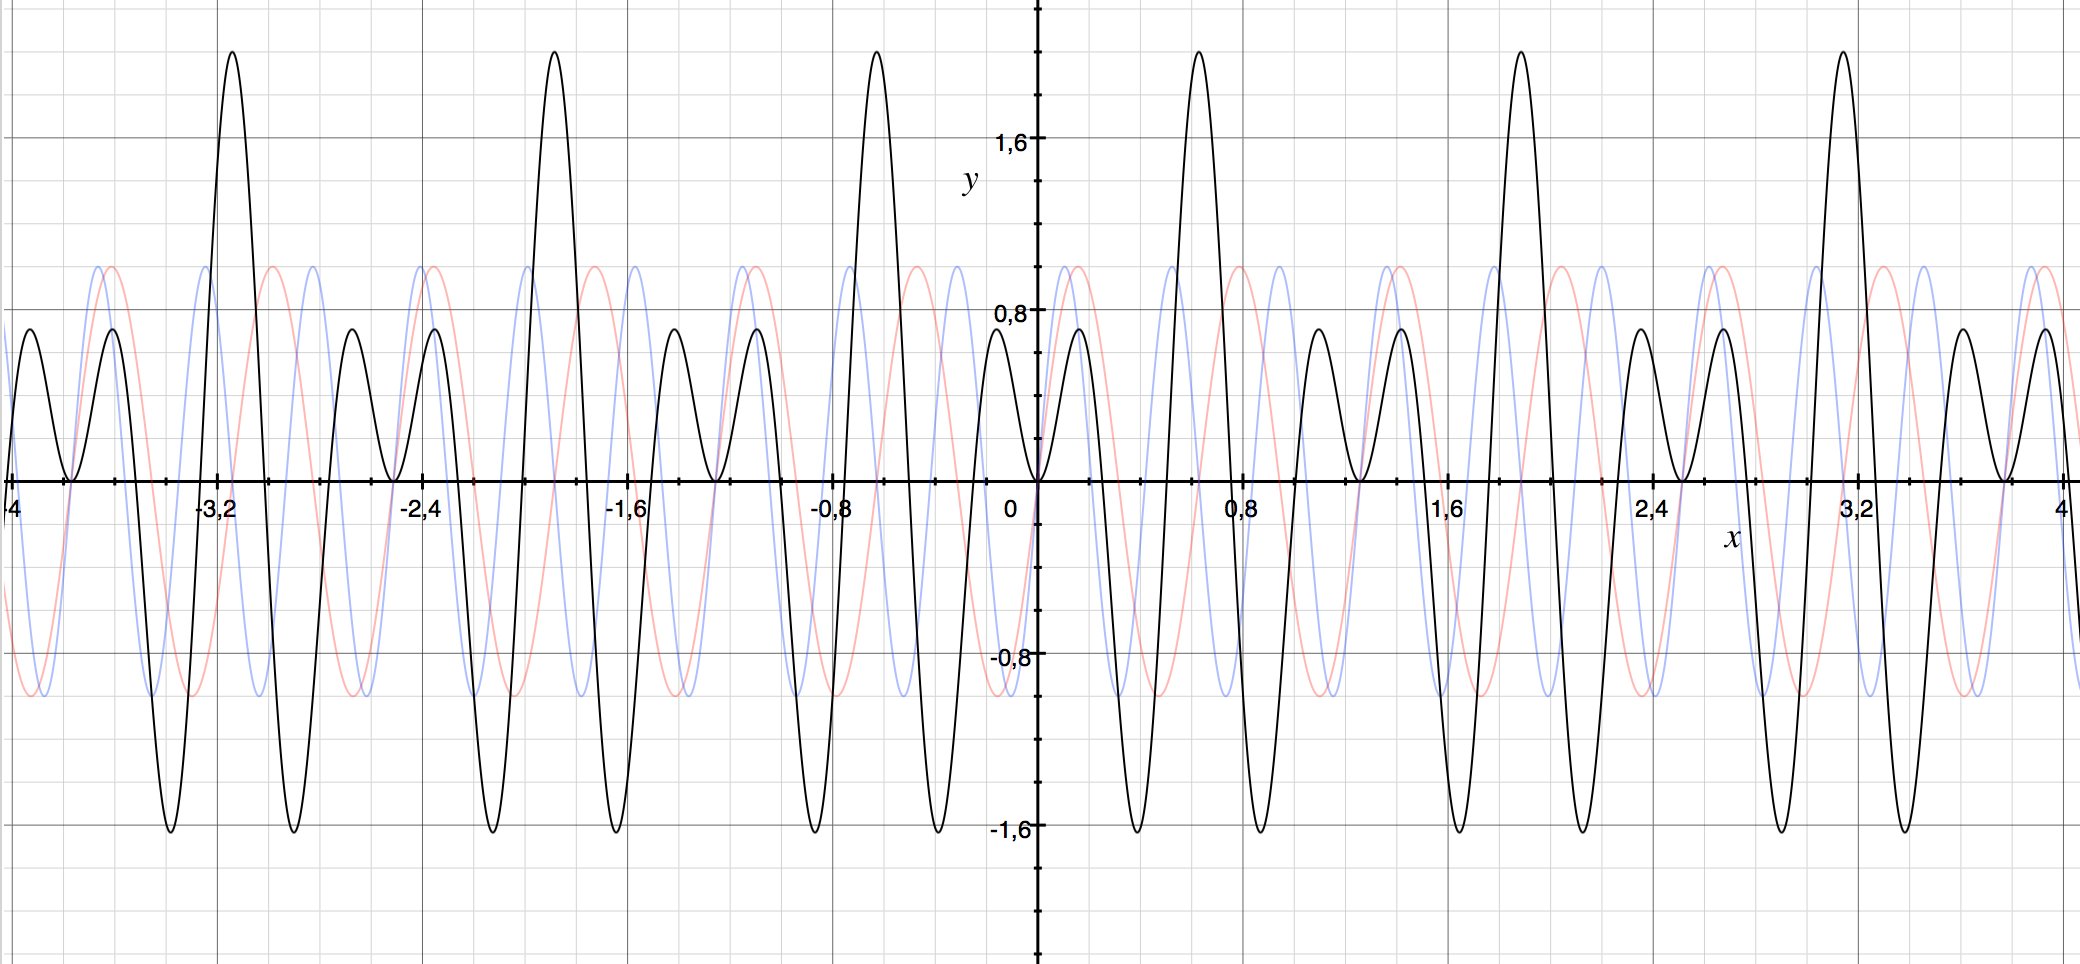
\includegraphics[scale=.4]{S3}
		\caption{Suma de las dos ondas anteriores, notemos que $\Delta \omega = 5$ y que por tato la onda suma será $y = 2 \sin(2.5 x) \sin(12.5 x)$}
	\end{figure}
	%\begin{center}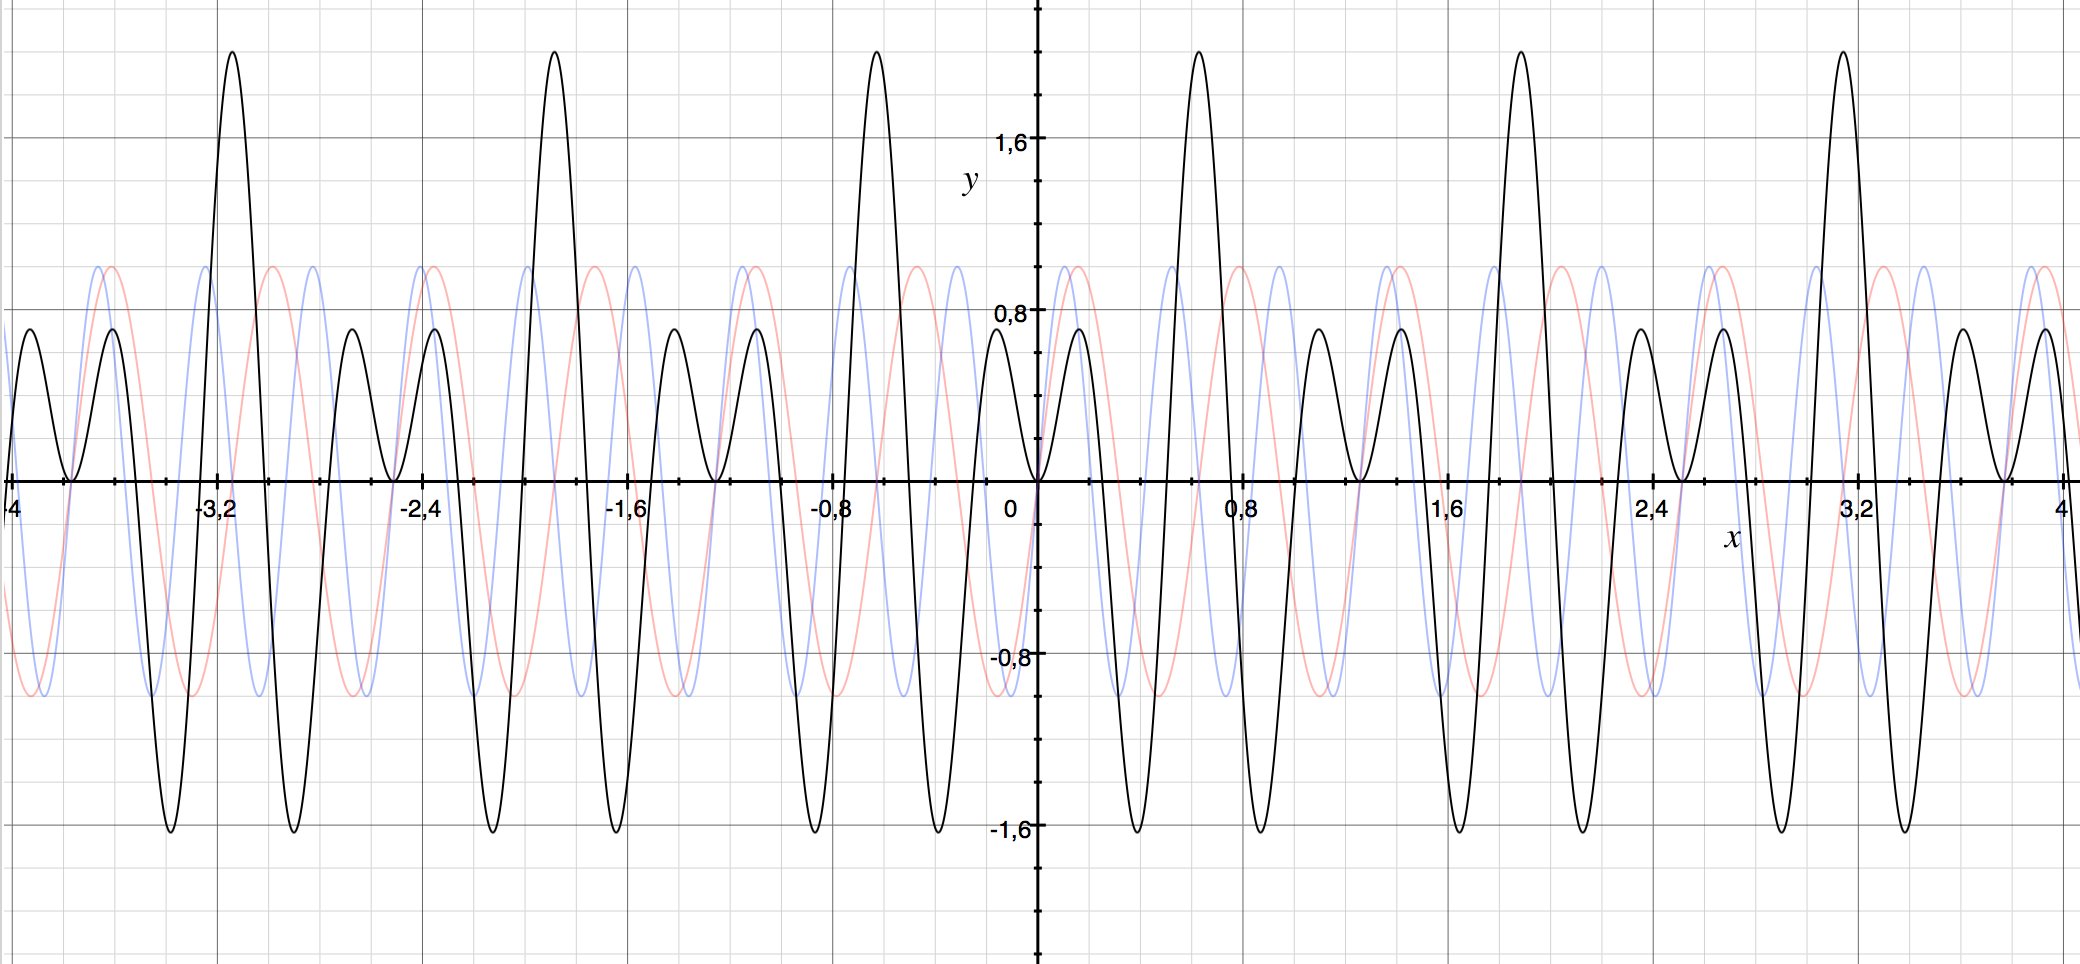
\includegraphics[scale=.3]{S3}\end{center}
	
	Es importante remarcar, que hasta llegar a los trabajos de R. Plomp y W.\,M. Levelt, hubo más gente desarrollando la teoría de los batidos de Helmholtz. Destacan \cite{PL} W. Preyer, quien ahondó en la idea de que los batidos son la base de la disonancia, F. Krueger, quien afirmó que los trabajos de Helmholtz subestimaban el efecto del tono en relación a la disonancia producida por los batidos y H. Sanding, quien comparó el carácter de los intervalos con dos tonos presentados al mismo tiempo en un único oído o, también al mismo tiempo, presentando cada uno de los tonos por uno de los oídos llegando a la conclusión de que en este último caso el intervalo presenta un carácter más neutral.
	
	\subsection{R. Plomp y W. J. M. Levelt}

	En abril de 1965 R. Plomp y W.\,M. Levelt publicaron su artículo ``Tonal Consonance and Critical Bandwidth''\cite{PL}. En él, a partir de datos experimentales, llegaron a establecer un modelo que nos ofrece una medida de la disonancia total entre sonidos.
		
	El experimento consistió en tomar un voluntario y, en condiciones plenamente controladas, someterle a la escucha de muestras de sonido conocidas, consistentes en un intervalo concreto. Después, el sujeto debería valorar dos aspectos de lo que ha escuchado: situación del intervalo en el rango de frecuencias (tomando como medida la media geométrica de las frecuencias de los dos tonos implicados) y diferencia de frecuencia entre los tonos. Los niveles de presión sonora se mantuvieron constantes a lo largo de todo el experimento. Cada sujeto participaba en el experimento una única vez y valoraba entre $12$ y $14$ muestras. Para no obtener ruidos en los datos, se excluyeron aquellas mediciones (todas las aportadas por un mismo sujeto) cuyos coeficiente de correlación indicaban que las respuestas no eran consistentes.
	
%	\begin{figure}[h]
%	    \centering
%	    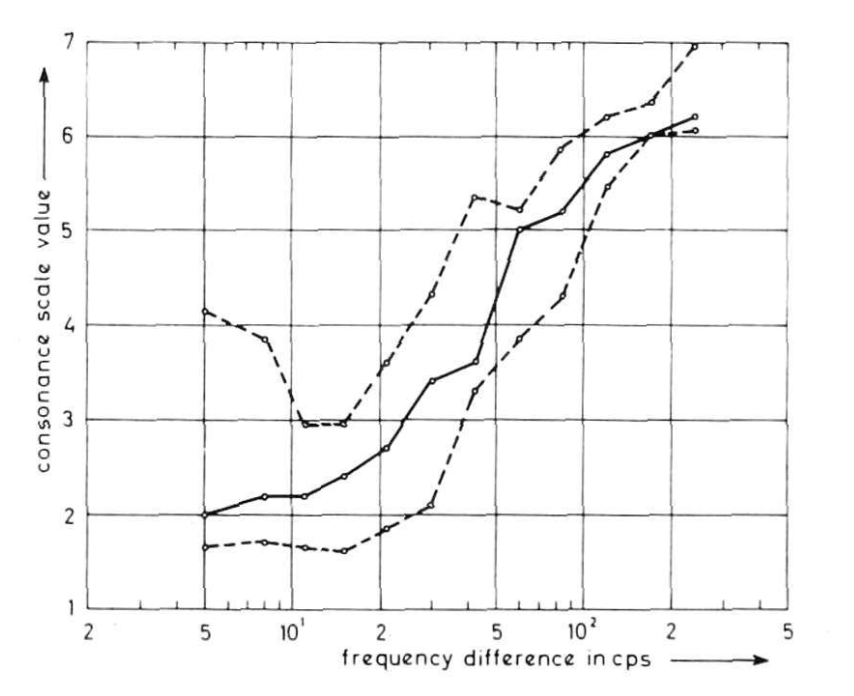
\includegraphics[scale=.75]{Datos1.png}
%	    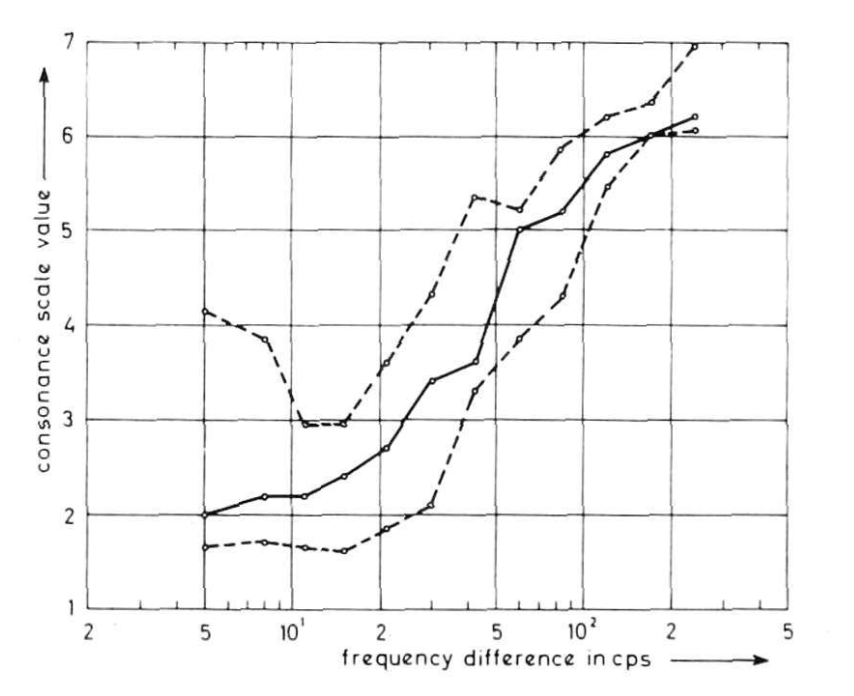
\includegraphics[scale=.75]{Datos1.png}
%	    \caption{Ambas figuras son originales del artículo de Plomp y Levelt\cite{PL}, se corresponden con los datos aportados por los sujetos de sus experimentos (10 sujetos por gráfico).}
%	\end{figure}
	
    \begin{center}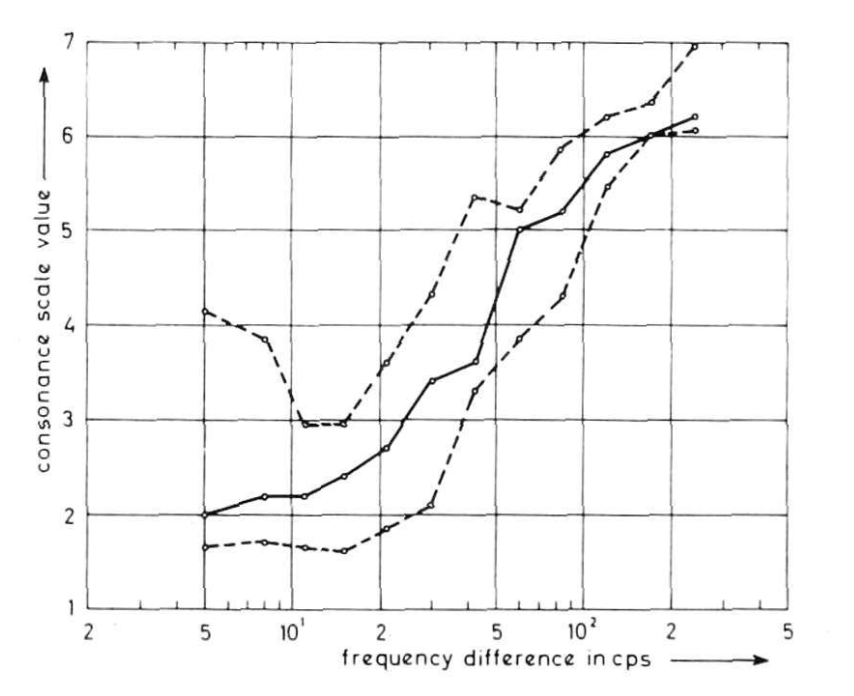
\includegraphics[scale=.75]{Datos1.png}\end{center}\\*
    
    \begin{center}Curvas originales del artículo de Plop y Levelt \cite{PL}, se corresponden con los datos aportados por los sujetos de sus experimentos. \end{center}\\*
	
	Los resultados no confirmaron la opinión de Helmholtz sobre la independencia de la máxima aspereza de la frecuencia. Los valores de $30-40$ cps aportados por él se encuentran en los datos experimentales solamente para frecuencias entre los $500$ y los $1000$ cps. La tendencia general de los datos indica que al aumentar la frecuencia el ancho del intervalo de máxima aspereza también aumenta. La diferencia de frecuencia (no fija) proporcional al ancho de banda crítica es la que mejor encaja con los datos experimentales.
	Análogamente podemos hablar de la mínima diferencia entre frecuencias que juzgamos como consonante.
	
	Estos experimentos también fueron repetidos para estimar la consonancia de más de un sonido.
	
	A partir de sus trabajos, estos autores diseñaron el modelo para estudiar la disonancia que se expondrán a continuación (primero para dos sonidos, luego para timbres, acabaré hablando de las superficies de disonancia).
	
	\subsubsection{Modelos de la disonancia}
	
		
	El elemento básico del estudio realizado por Sethares son las \emph{curvas de Plomp-Levelt}, que parametrizaremos utilizando el modelo:

    $$ d(x) = e^{-b_1 x} -  e^{-b_2 x} $$

    Donde $x$ se define como:
    
    $$
        x_{i,j} = x (f_i, f_j) := \frac{| f_i - f_j |}{\min{f_i, f_j}}
    $$
    
    Utilizando minimización gradiente del error cuadrado entre los datos y la curva: $b_1 = 3.5$ y $b_2 = 5.75$. \\*

 %   \begin{figure}[h]
%    	\centering
 %   	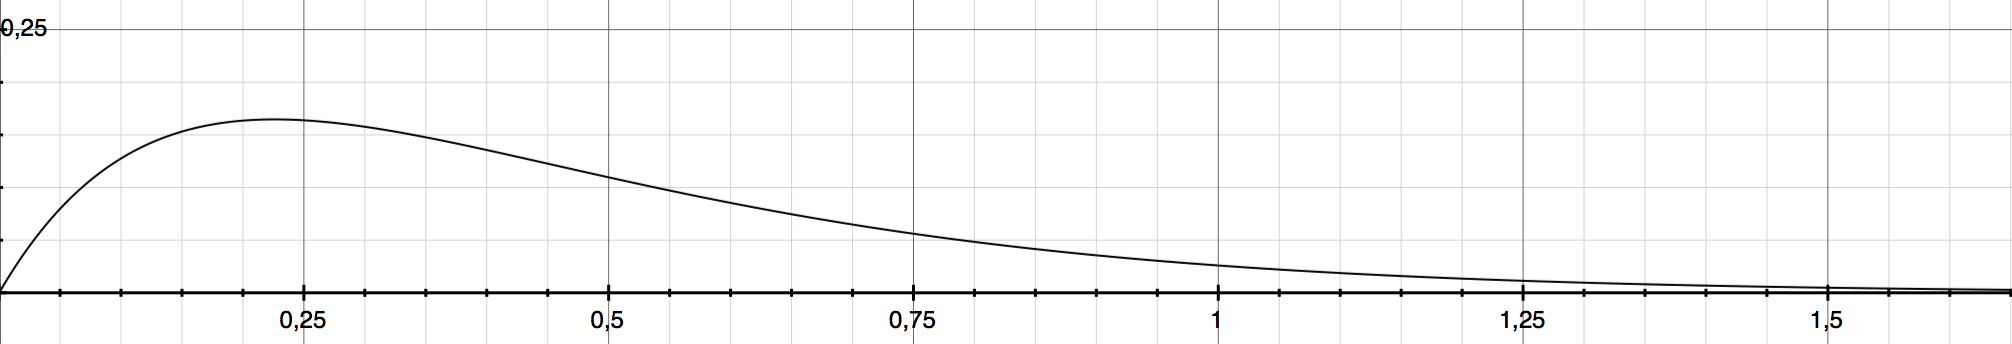
\includegraphics[scale=0.4]{CDisonancia2}
%    	\caption{Modelo para los valores $b_1 = 3.5$ y $ b_2 = 5.75$}
 %   \end{figure}
    
    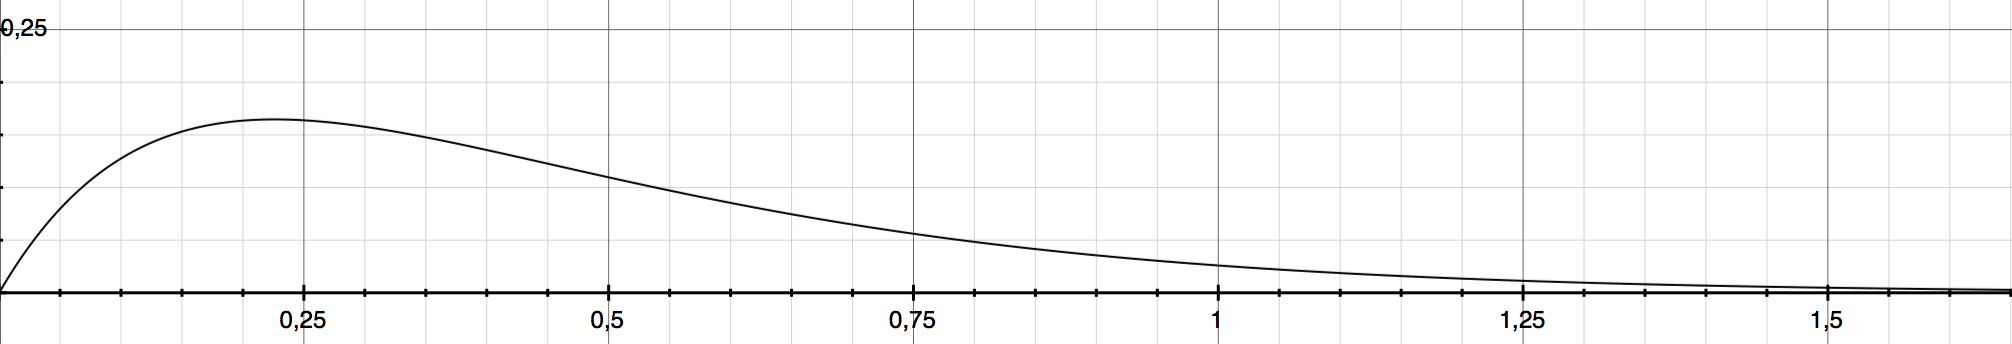
\includegraphics[scale=0.4]{CDisonancia2} \\*
    
    La curva de disonancia puede ser escalada para representar convenientemente curvas de diferentes amplitudes y frecuencias. Si el \textit{punto de máxima disonancia} ocurre en $x^{*}$, entonces la disonancia entre las frecuencias $f_1$ y $f_2$ ($f_1 < f_2$) de amplitudes respectivas $l_1$ y $l_2$ es:
    
    $$
        \boxed{
            d(f_1, f_2, l_1, l_2) = l_{12} [e^{-b_1 s (f_2 - f_1)} -  e^{-b_2 s (f_2 - f_1)}
        }
    ]$$
 
    Donde:
    
    $$
        l_{12} =\min(l_1, l_2)
    $$
    
    $$ 
        s = \frac{x^{*}}{s_1 f_1 + s_2}
    $$
    
    Siendo $x^{*} = 0.24$, $s_1 = 0.021$ y $s_2 = 19$.

    Se observa que la forma de la ecuación nos garantiza que los componentes más suaves contribuyen menos que los más fuertes, provocando así que en el caso de sonidos débiles la disonancia prácticamente desaparezca.

    Calcular la intensidad del sonido no es trivial. Sea $p(t)$ una onda simple armónica plana con periodo $T$, entonces la \emph{presión efectiva} es:
    
    $$
        P_e = \sqrt{\frac{1}{T} \int_{0}^{T}{p^{2}(t) dt}} 
    $$

    Para una onda sinusoidal $ p(t) = A \sin{(2 \pi f_0 t + \phi)} $ de frecuencia $f_0$ y amplitud $A$, 
    $P_e = \frac{A} {\sqrt{2}}$ La \emph{presión del sonido en Decibelios (dB)},
    $ SPL = 20 \log_{10}{\frac{P_e}{P_{ref}}}$, donde $P_{ref}$ es el estándar $20 \mu Pa^{2}$ $SPL$ en el aire, que se corresponde con el $SPL$ de una onda apenas audible de $1000 Hz$. Finalmente la \emph{intensidad} se puede aproximar mediante:
    $$ l = \frac{1}{16} 2^{\frac{SPL}{10}} $$
    La Intensidad se mide en \emph{sones}.

    Observemos que, aproximadamente, un incremento de $10 dB$ implica doblar la intensidad. El coeficiente $\frac{1}{16}$ normaliza la intensidad, de tal manera que $40 dB$ equivale a $1 sones$.
      
    
    
    
    
    
    \subsubsection{Curvas de disonancia}
    
    Para continuar con el estudio de la disonancia de tonos más complejos necesitaremos definir varios conceptos.
    
    
    \noindent\textbf{Definición:} Llamamos \emph{timbre} o \emph{espectro}, $\mathfrak{F}$, a una colección de $n$ frecuencias $f_1 < f_2 < ... < f_n$ con sus respectivas amplitudes $l_1, l_2,... , l_n$. 
  
    
     $$
        \mathfrak{F} := \{ (f_i, l_i) : i = 1,...,n \}
     $$
        
    Si las amplitudes no son relevantes, o por alguna razón su valor está implícito (como por ejemplo si todas valen $1$, circunstancia que contemplaremos en casi todos los puntos del trabajo), escribiremos el espectro por simplicidad como:
    
    $$
        \mathfrak{F} := \{ f_i : i = 1,... ,n \}
    $$
    
    \noindent\textbf{Definición:} Llamaremos \emph{frecuencia fundamental o fundamental} de un espectro a la frecuencia más importante de un espectro Típicamente será aquella cuya amplitud sea mayor. El resto de frecuencias que conforman el espectro se denominan \emph{parciales}.
      
    \noindent\textbf{Definición:} Llamaremos \emph{espectro armónico de una frecuencia fundamental $f_1$} a aquel cuyas frecuencias parciales son múltiplos enteros de la frecuencia fundamental.
    
    $$
        \mathfrak{F}_{A} := \{ f_k :  f_k := k f_1, \, k \in \mathbb{N}, \, k \leq n \}
    $$
      
    \noindent\textbf{Definición:} Llamaremos \emph{espectro armónico estirado de una frecuencia fundamental $f_1$} a uno construído de la siguiente forma:
    
    $$
        \mathfrak{F}_{A}^{s} := \{ f_k :  f_k := k^{s} f_1, \, k \in \mathbb{N}, \, k \leq n \}
    $$
    
    Observemos que: $ \mathfrak{F}_{A}^{1} = \mathfrak{F}_{A} $
    
    
    \noindent\textbf{Definición:} La  \emph{Disonancia intrínseca o inherente de $\mathfrak{F}$} se define como la suma de las disonancias de todos los pares de ondas del conjunto:
    
    $$
        D_{\mathfrak{F}} := \frac{1}{2} \sum_{i = 0}^{n}{ \sum_{j = 0}^{n}{ d(f_i, f_j, l_i, l_j) } } 
    $$

    Cuando queremos calcular la disonancia intrínseca de dos notas de espectro $\mathfrak{F}$ separadas por un intervalo $\\alpha$ procedemos como si de un único espectro se tratase que incluya, por adicción, las frecuencias $f_i$ y $\alpha f_i$. Así:
    
    $$ 
        D_{\mathfrak{F}} (\alpha) := D_{\alpha} + D_{\alpha \mathfrak{F}} + \sum_{i= 0}^{n} { \sum_{j= 0}^{n}{ d(f_i, \alpha f_j, l_i, l_j)}} 
    $$

    \noindent\textbf{Definición:} La \emph{Curva de Disonancia generada por el Timbre $\mathfrak{F}$} es definida como la función $D_{\mathfrak{F}}(\alpha)$ sobre todos los intervalos de interés en $\alpha$.

    La \emph{Disonancia de un acorde de tres notas a intervalos $1, r$ y $s$} se calcula de manera similar añadiendo las disonancias entre las parciales:
    
    $$ 
        D_{\mathfrak{F}}(r, s) := D_{\mathfrak{F}}(r) + D_{\mathfrak{F}}(s) + D_{r \mathfrak{F}} \left( \frac{s}{r} \right) 
    $$
    
    Donde $D_{r \mathfrak{F}}(\frac{s}{r})$ es la disonancia entre $r \mathfrak{F}$ y $s \mathfrak{F}$.

    La forma de la curva depende de las frecuencias y magnitudes del espectro. Cambios en cualquiera de las anteriores cambiarán las localizaciones de los mínimos de la curva y sus profundidades.
    
    Estas curvas de disonancia tienen $4$ propiedades básicas. En adelante, consideraré estas como \emph{las propiedades que cualquier modelo que explique la disonancia deberá tener}.
    
    
    \noindent\textbf{Propiedad $1$:} El unísono es el mínimo de la curva de disonancia.
      
    \noindent\textbf{Propiedad $2$:} Al crecer el intervalo, el valor de la disonancia se aproxima a la disonancia intrínseca del sonido.
    
    \noindent\textbf{Propiedad $3$:} La curva generada por el timbre $\mathfrak{F}$ tiene al menos $2n^2$ mínimos localizados simétricamente (en una escala logarítmica), entonces la mitad de ellos se encuentran entre $0$ y $1$ y la otra mitad entre $1$ e infinito.
    
    \noindent\textbf{Propiedad $4$:} \emph{Principio de las parciales coincidentes}. $n^2$ de los mínimos ocurren en intervalos de razón $r = f_i /f_j$, donde $f_i$ y $f_j$ son parciales de $\mathfrak{F}$
    % up to n^2 of the minima are the broad type of the bottom curve in fig.6.15 pg 123
    

    \subsubsection{Superficies de disonancia}
    
    Las curvas de disonancia también pueden ser dibujadas para ``acordes'' de $3$ notas. Estas curvas se convertirán en superficies donde los máximos y mínimos de la superficie indicarán de nuevo los puntos de máxima y mínima disonancia respectivamente. Como anteriormente, la disonancia total se calculará sumando las disonancias entre todas las parciales. \\*
    
    La disonancia de un acorde de tres notas de espectros $\mathfrak{F}$, $r\mathfrak{F}$ y $s\mathfrak{F}$ es:
    
    $$
        \{\hbox{Disonancia total del acorde}\} 
    $$
    $$
    = \{\hbox{Disonancia entre } \mathfrak{F} \hbox{ y } r\mathfrak{F}\} +\{\hbox{Disonancia entre } \mathfrak{F} \hbox{ y } s\mathfrak{F}\} +\{\hbox{Disonancia entre } r\mathfrak{F} \hbox{ y } s\mathfrak{F}\} 
    $$
    
    Es posible generalizar la idea para $N$ sonidos sonando simultáneamente. Esta idea es interesante de cara a buscar los máximos y mínimos del sonido formado por los $N$ sonidos individuales, aunque para $m>2$ no podamos visualizarlo tan fácilmente.
    

	\newpage
	
%%%%%%%%%%%%%%%%%%%%%%%%%%%%%%%%%%%%%%%%%%%%%%%%%%%%%%%%%%%%%%%%%%%%%%%%%%%%%%	

\section{Estudio de las curvas de disonancia}
    
    	


	\subsection{Estudio teórico del modelo de Sethares:}
	El objeto de esta sección es demostrar que el modelo utilizado por Sethares cumple las propiedades básicas de las curvas de disonancia.
	
	\begin{teor}                      %% TEOREMA 1 %%
	Para cualquier timbre $\mathfrak{F}$ con parciales $f_1, f_2,... , f_n$: $$\lim_{\alpha \rightarrow \infty}{D_{\mathfrak{F}}(\alpha)} = D_{\mathfrak{F}} + D_{\alpha \mathfrak{F}}$$ 
	\end{teor}
	
	\noindent\textbf{Demostración:} 

Claramente $d(x) \rightarrow 0$ si $x \rightarrow \infty$.

Entonces $d(f_i, \alpha f_j) \rightarrow 0$ para cuales quiera i,j cuando $\alpha \rightarrow \infty$. 

Ello implica que la doble suma tiende a 0.       

$\blacksquare$

Observemos que esto implica que la disonancia tiende a 0 cuando el intervalo $\alpha$ crece.

Varios aspectos de las curvas de disonancias se tornan importantes cuando investigamos la localización de los posibles mínimos de la curva. 

Derivando e igualando a cero, obtenemos el punto de \emph{máxima disonancia} para el valor : 

 $$
    x^{*} = \frac{\ln(\frac{b_1}{b_2})}{b_1-b_2}
 $$

Antes de proseguir, enunciaremos una hipótesis que será utilizada en los siguientes teoremas.Decimos que dos parciales, $f_1$ y $f_2$, están \emph{separadas por $x^{*}$} si:

$$
    x = \frac{ | f_1 - f_2 | }{\min(f_1, f_2) > x^{*}} 
$$


El cambio en disonancia en $x = 0$ es:

$$
    d'(0) = -b_1 e^{-b_1 x} + b_2 e^{-b_2 x} |_{x = 0} = b_2 - b_1 
$$

Para $ x > x^{*} $, el máximo cambio en la disonancia ocurre cuando $ d''(x^{**})$ es mínimo.
$$ d''(x) = b_1^2 e^{-b_1 x} - b_2^2 e^{-b_2 x}$$
Después de simplificaciones...
$$ x^{**} = \frac{2 \ln\left(\frac{b_1}{b_2}\right)}{b_1 - b_2} $$
Que es donde se alcanza el mínimo. Después de simplificaciones el valor de $d'$ en $x^{**}$ es:
$$ d'(x^{**}) = b_2 \left(\frac{b_1}{b_2}\right)^{\frac{2 b_2}{b_1 - b_2}} - b_1 \left(\frac{b_1}{b_2}\right)^{\frac{2 b_1}{b_1 - b_2}}    $$

Los valores usados son $b_1 \approx 3.5$ y $b_2 \approx 5.75$, $x^{*} \approx 0.22$, $d'(0) \approx 2.25$, $x^{**} \approx 0.44$ y $d''(x^{**}) \approx -0.292$, aunque generalmente con tomar $b_2 > b_1 > 0$ es suficiente.

El siguiente resultado nos da las condiciones bajo las cuales el \emph{unísono}, es decir, $\alpha = 1$, es un mínimo de la curva de disonancia $D_{\mathfrak{F}} (\alpha)$.

%%%%%%%%%%%%%%%%%%%%%%%%%%%%%%%%%%%%%%%%%%%%%%%%%%%%%%%%%%%%%%%%%%%%%%%%%%

	\begin{teor}                      %% TEOREMA 2 %%	
	Supongamos el timbre $\mathfrak{F}$ con parciales $f_1< f_2 <... < f_n$ separadas todas ellas por al menos $x^{*}$. Entonces $\alpha = 1$ es un mínimo de la curva de disonancia $D_{\mathfrak{F}}(\alpha)$.
	\end{teor}

    El teorema es cierto, sin embargo, como analizaremos en uno de los apartados del apéndice, la demostración dada por el autor es errónea.
    
    Este teorema se podría enunciar como un corolario del teorema demostrado en la sección ``Resultados propios'', pues las curvas de Plomp Levelt usadas en él son un caso particular de las curvas de disonancia para las que el teorema en esa sección presentado es cierto.

%%%%%%%%%%%%%%%%%%%%%%%%%%%%%%%%%%%%%%%%%%%%%%%%%%%%%%%%%%%%%%%%%%%%%%%%%%

	\begin{teor}                      %% TEOREMA 3 %%
	Sea $\mathfrak{F}$ un timbre con parciales $f_1$ y $f_2$ separadas al menos por $x^{*}$. Entonces la curva de disonancia $D_{\mathfrak{f}}(\alpha)$ tiene un mí­nimo en $\alpha^{*} = \frac{f_2}{f_1}$.
	\end{teor}
	
	\noindent\textbf{Demostración:} 

Sea $\mathfrak{G}$ timbre con parciales $(g_1, g_2) = (\alpha f_1, \alpha f_2)$. Entonces $D_{\mathfrak{F}} = D_{\mathfrak{G}} = D_{\alpha \mathfrak{F}} $ y cualquier cambio en $D_{\mathfrak{F}} (\alpha)$ debe originarse en el doble sumatorio, que contiene los términos $d(f_i, g_j)$  para $i = 1, 2$ y $j = 1, 2$.\\
Para $\alpha^{*} = \frac{f_2}{f_1}$, $d(g_1, g_2) = d(f_2, \alpha f_2)$. Como $\alpha$ es perturbado por $\alpha^{*}$, la contribución del término $d(f_2, g_1) = d(f_2, \alpha f_1)$ crece, porque en $\alpha^{*}$, $\alpha^{*} f_1 = f_2$ y entonces $d(f_2, g_1) = d(f_2, f_2) = 0$.

Entonces el resultado puede ser demostrado probando que el inrcemento en $d(f_2, g_1)$ es mayor que el decremento en los otros tres términos combinados. 

El incremento en $d(f_2, g_1)$ es proporcional a $d'(0)$. Como $f_1$ y $f_2$ están separados por $x^{*}$, el decremento en cada uno de los otros tres términos no es mayor que $d'(x^{**})$.  Como $| d'(0) | > 7 | d'(x^{**}) | $. Esto prueba el resultado.
$\blacksquare$

Entonces la curva de disonancia generada por las parciales $f_1$ y $f_2$ alcanza un mínimo cuando $\alpha^{*} f_1 = f_2$. Por ejemplo, para un timbre $\mathfrak{F}$ con parciales $(500, 750), \alpha^{*} = 1.5$. El resultado afirma que el timbre $\alpha^{*} \mathfrak{F}$, con frecuencias $(750, 1125)$ es localmente un intervalo más consonante. En símbolos: $D_{\mathfrak{F}}(\alpha^{*} - \epsilon) > D_{\mathfrak{F}}(\alpha^{*})$ y 
$D_{\mathfrak{F}}(\alpha^{*} + \epsilon) > D_{\mathfrak{F}}(\epsilon^{*})$. Entonces ambos $(748, 1122)$ y $(752, 1128)$ son menos consonantes que $(750, 1125)$. Este resultado es intuitivo porque cuando $\alpha f_1 \neq f_2$, la disonancia entre las parciales en $\alpha f_1$ y $f_2$ es grande, pero cuando $\alpha f_1 = f_2$, este término desaparece de la medida de la disonancia.

%Es interesante que este resultado puede fallar cuando $f_1$ y $f_2$ están muy cerca.  

%%%%%%%%%%%%%%%%%%%%%%%%%%%%%%%%%%%%%%%%%%%%%%%%%%%%%%%%%%%%%%%%%%%%%%%%%%

	\begin{teor}                      %% TEOREMA 4 %%
	Sea $\mathfrak{F}$ un timbre con parciales $f_1$ y $f_2$. Entonces $\exists \epsilon > 0$ tal que si $\vert f_1 - f_2 \vert < \epsilon$, el punto $\epsilon^{*} = \frac{f_2}{f_1}$  no es un mí­nimo de la curva de disonancia $D_{\mathfrak{F}}(\alpha)$.
	\end{teor}
	
	\noindent\textbf{Demostración:} \ 
Definimos $\mathfrak{G}$ como en el teorema enterior.\\
De nuevo, cualquier cambio en $D_{\mathfrak{F}}(\alpha)$ es el resultado de los cuatro términos de la suma (Teorema 2).  Para un $\epsilon > 0 $ pequeño nótese que $d(f_1, g_1 + \epsilon) > d(f_1, g_1) > d(f_1, g_1 - \epsilon)$, $d(f_1, g_2 + \epsilon) > d(f_1, g_2) > d(f_1, g_2 -\epsilon)$
, $d(f_2, g_2 + \epsilon) > d(f_2, g_2) > d(f_2, g_2 - \epsilon)$ y $d(f_2, g_1 + \epsilon) > d(f_2, g_1)$. \\
Por otra parte: $d(f_2, g_1 - 	\epsilon) > d(f_2, g_1) = d(f_2, f_2) = 0$.\\
Para $\epsilon $ pequeños el cambio en los cuatro términos es de aproximadamente magnitud $	\epsilon(b_2 - b_1)$. Entonces el valor en la disonancia decrece al acercar $\mathfrak{G}$ $\epsilon$ a $\mathfrak{F}$, y $\alpha^{*} = \frac{f_2}{f_1}$ no es un mínimo.\\
$\blacksquare $  

En esencia, si las parciales $f_1$ y $f_2$ están muy cerca, el mínimo $\frac{f_2}{f_1}$ desaparece.\\
El Teorema 3 nos muestra que el mínimo ocurre cuando las parciales coinciden. El mínimo puede también ocurrir cuando las parciales están ampliamente separadas. Para un timbre $\mathfrak{F}$ de dos parciales, supongamos que $f_1$ y $f_2$ están separadas al menos por $4x^{*}$, entonces hay un intervalo de máxima disonancia cerca $\alpha f_1 = f_1 + x^{*}$  y cerca $\alpha f_2 = f_2 - x^{*}$. Consecuentemente, debe haber algún mínimo para algún $\alpha$ entre $\alpha_{L} = \frac{f_1 + x^{*}}{f_1}$ y $\alpha_{H} = \frac{f_2 - x^{*}}{f_2}$. 

%El Teorema 4 sugiere que el mínimo de la curva de disonancia con poca probabilidad se encuentra en un intervalo más pequeño que la mitad de $x^{*}$ en donde %máxima disonancia ocurre. Plomp yLevelt estima que $x^{*}$ corresponde a un poco menos que $\frac{1}{3}$ de la bande crítica. Entonces el Teorema 4 predice que %pasos de la escala cercanos entre ellos más de $\frac{1}{6}$ de la banda crítica deberían ser raros.

El siguiente resultado describe el mínimo de la curva de disonancia para timbres con tres parciales.

%%%%%%%%%%%%%%%%%%%%%%%%%%%%%%%%%%%%%%%%%%%%%%%%%%%%%%%%%%%%%%%%%%%%%%%%%%

	\begin{teor}                      %% TEOREMA 5 %%
	Sea $\mathfrak{F}$ un timbre con parciales $f_1, f_2$ y $f_3$. $\exists c_1, c_2 > 0$  tales que si $f_1$ y $f_2$ están separados al menos por $x^{*} + c_1$ y $f_2$ y $f_3$ al menos por $x^{*} + c_2$, entonces los mínimos de la curva de disonancia se alcanzan en $\alpha_1 = \frac{f_2}{f_1}$, $\alpha_2 = \frac{f_3}{f_1}$ y $\alpha_3 = \frac{f_3}{f_2}$.
	\end{teor}

\noindent\textbf{Demostración:} 

Sea $\mathfrak{G}$ timbre de parciales $(g_1, g_2, g_3) = (\alpha f_1, \alpha f_2, \alpha f_3)$. Supongamos primero que $f_2 - f_1 > f_3 - f_2 + c_2$.

Consideremos el candidato a mínimo. $\alpha_1$. Para un $\epsilon$ pequeño, los valores más significativos en $D_{\mathfrak{F}}(\alpha - \epsilon) - D_{\mathfrak{F}}(\alpha)$ son $d(f_2, g_1)$ y $d(f_3, g_2)$, porque todos los demás están separados al menos por $x^{*} + c_2$.

Para $\epsilon > 0$, $d(f_2, g_1 + \epsilon) > d(f_2, g_1), d(f_3, g_2 + \epsilon) > d(f_3, g_2)$ y $d(f_2, g_1 - \epsilon) > d(f_2, g_1)$. Por otro lado $d(f_3, g_2 - \epsilon) <  d(f_3,g_2)$.

Pero $d'(0) = b_2 - b_1$ y $d''(0) = b_1^2 - b_2^2  < 0 $, entonces la pendiente está decreciendo. Entonces $ \vert d(f_2, g_1 - \epsilon) \vert > \vert d(f_3, g_2 - \epsilon) \vert$.

Consecuentemente: $D_{\mathfrak{F}} (\alpha_1 + \epsilon) > D_{\mathfrak{F}} (\alpha_1) $ y $ D_{\mathfrak{F}} (\alpha_1 - \epsilon) > D_{\mathfrak{F}} (\alpha_1) $, mostrando que $\alpha_1$ es un mínimo local.
 
Con el caso $f_3 - f_2 > f_2 - f_1 + c_1$ se procede de igual manera.

Las pruebas para $\alpha_2$ y $\alpha_3$ son similares.

$\blacksquare$

El resultado final especifica el máximo número de mínimos que puede tener una curva de disonancia en términos de la complejidad del espectro del sonido.

%%%%%%%%%%%%%%%%%%%%%%%%%%%%%%%%%%%%%%%%%%%%%%%%%%%%%%%%%%%%%%%%%%%%%%%%%%

	\begin{teor}                      %% TEOREMA 6 %%
	Sea $\mathfrak{F}$ un timbre de parciales $f_1, f_2,... , f_n$. Entonces la curva de disonancia $D_{\mathfrak{F}}(\alpha)$ tiene al menos $2 n^{2}$ mínimos locales.
	\end{teor}
	
	\noindent\textbf{Demostración:} 

Consideremos la porción de $D_{\mathfrak{F}}(\alpha)$ debida  la parcial $f$ interactuando con la parcial fija $f_j$. Para ambas un muy pequeño ($\alpha (\alpha \approx 0)$ y un muy grande $\alpha (\alpha \rightarrow \infty)$, $d(\alpha f, f_j) \approx 0$.

En $\alpha = \frac{f_j}{f}$, $d(\alpha f, f_j) = 0$ . Para los dos intervalos donde $ \alpha f $ y $ f_j $ están separados por $ x^{*}$ (una con $ \alpha f < f_j $ y otra con $ \alpha f > f_j$), $d(\alpha f, f_j)$ alcanza su valor máximo.

Entonces $f$ interactuando con un $f_j$ fijo tiene dos máximos y un mínimo.

Cada $f_i$ puede interactuar con cada $f_j$, y hay $n^2$ posibles parejas.
 
Como $D_{\mathfrak{F}}(\alpha)$ consiste en $n^2$ curvas sumadas juntas, hay como mucho $2n^2$ máximos.

Consecuentemente, no puede haber más de $2n^2$ mínimos. Los extremos mínimos de $\alpha = 0$ y $\alpha = \infty$ no están incluídos.

$\blacksquare$

A pesar de los detalles de la presentación, su conclusión principal es que el mínimo más útil (musicalmente) de la curva de disonancia tiende a estar localizado en el intervalo $\alpha$ donde $f_i = \alpha f_j$, donde $f_i, f_j$ son parciales arbitrarias del timbre $	\mathfrak{F}$.

Los \emph{Teoremas de esta sección asumen que todas las parciales tienen la misma amplitud}. El efecto de amplitudes no iguales es que algunas no mínimas tienden a desaparecer, , algunas pueden aparecer y otras pueden cambiar de frecuencia. Afortunadamente estos cambios ocurren de manera estructurada.

Concretamente, sea $\mathfrak{F}$ un timbre con parciales $f_1, f_2,... , f_n$ de amplitudes relativas $a_1, a_2,... , a_n$ y sea $\mathfrak{\widehat{F}}$ un timbre con las mismas parciales pero todas con amplitud $1$. 

Por lo dicho arriba la curva de disonancia para $\mathfrak{\widehat{F}}$ tiene hasta $n^2$ debido a las coincidencias en las parciales en los intervalos $\alpha_{ij} = \frac{f_i}{f_j}$.

Como las amplitudes $a_j$ en $\mathfrak{F}$ se mueven de la unidad, la profundidad de la curva de disonancia en $\alpha_{ij}$ puede cambiar y el mínimo en alguno de los $\alpha_{ij}$ puede desaparecer (un $\alpha_{ij}$ mínimo en $D_{\mathfrak{\widehat{F}}}$ puede no ser mínimo en $D_{\mathfrak{F}}$), y otros $\alpha_{ij}$ pueden aparecer (similar al caso anterior).

Entonces, variaciones en la amplitud de las parciales tienden a afectar al hecho de que los $\alpha_{ij}$ sean mínimos. La curva de disonancia también contiene hasta $n^2$ mínimos del tipo "ancho". La localización de esos equilibrios es menos cierta, porque estos se mueven continuamente con respecto a las variaciones en la amplitud $a_j$.

\subsubsection{Otros resultados sobre el modelo de Sethares}

    Los siguientes resultados hacen referecia al modelo que parametriza la función de disonancia mediante las curvas de Plomp-Levelt:
    
    $$
        d(x) = e^{-b_1 x} - e^{-b2 x}
    $$
    
    En este modelo concreto tomamos como valores $b_1 = 3.5$ y $b_2 = 5.75$.
    
    Observemos que $d \in \mathcal{C}^{\infty} (0, +\infty)$.
    
\noindent\textbf{Resultado 1:} en este modelo se cumple $d^{(n)} (n x^{*}) = 0$. Es decir, que el punto donde se anula la derivada $n$-ésima es $n$ veces el punto donde se anula la primera derivada.

\noindent\textbf{Demostración:}

Primero calcularemso la derivada $n$-ésima, después llamaremos al punto donde esta, de hacerlo, se anula y para concluir comprobaremos que ese punto es $n$ veces el punto donde se anula la primera, que recordemos, es:

\begin{equation*}
    x^* = \frac{\ln  \left( {\frac{ b_1}{b_2}} \right) }{b_1 - b_2}
\end{equation*}

La derivada $n$-ésima es:

\begin{equation}
    d^{(n)} (x) = (-1)^{n} b_{1}^{n} e^{-b_1 x} - (-1)^{n} b_{2}^{n} e^{-b_2 x}
\end{equation}

Sea $y$ el punto donde se anula la derivada.

\begin{equation*}
    b_{1}^{n} e^{-b_1 y} = b_{2}^{n} e^{-b_2 y}
\end{equation*}
\begin{equation*}
    \left( \frac{b_1}{b_2} \right)^{n} = \left( \frac{e^{-b_2 y}}{e^{-b_1 y}} \right)
\end{equation*}
\begin{equation*}
    %\ln{\left( \frac{b_1}{b_2} \right)^{n}} =
    n \ln{\left( \frac{b_1}{b_2} \right)} = (b_1 - b_2) y
\end{equation*}
\begin{equation*}
    \Rightarrow y = n \frac{ \ln{\left( \frac{b_1}{b_2} \right)}}{b_1 - b_2} = n x^{*}
\end{equation*}
\begin{equation}
    \Rightarrow d^{(n)} (y) = d^{(n)} (nx^{*}) = 0
\end{equation}
\blacksquare
\newpage
\noindent\textbf{Resultado 2:} 
\begin{enumerate}
    \item $d^{(n)}$ si $n$ es par alcanza su máximo en el punto $(n+1)x^{*}$ y además $d^{(n)} ((n+1)x^{*}) > 0$. 
    \item $d^{(n)}$ si $n$ es impar alcanza su mínimo en el punto $(n+1)x^{*}$ y además $d^{(n)} ((n+1)x^{*}) < 0$.
\end{enumerate}

\noindent\textbf{Demostración:}

Teniendo presente el resultado anterior lo único que resta demostrar es que la alternancia entre máximos y mínimos se sucede de la forma indicada.

Observemos que, a la izquierda de $x^{}*$ tenemos que $d'(x) < 0$ y decreciente hasta el punto donde la derivada $d''$ vale $0$. A la derecha de $2X^{*}$ la función $d''$ será creciente ($d''' (x) > 0$). Por tanto $d'$ tendrá un mínimo en $2x^{*}$.

Basta extender el razonamiento anterior tomando la $n$-ésima derivada y sus siguientes derivadas para obtener el resultado.

\blacksquare

%\noindent\textbf{Resultado 3}: si tenemos una suma finita de curvas de Plomp-Levelt,  %$f(x) = \sum_{i = 1}^{N} e^{-a_i x}$ donde $a_i \geq o \, \forall a_i \in \mathbb{R}$, %se cumple:
%\begin{equation*}
%    f^{(n)} (nx^{*}) = 0
%\end{equation*}
%Este resultado es el análogo para la suma de curvas de Plomp-Levelt del resultado %número $1$.

%\noindent\textbf{Demostración:}

%Seguiremos el mismo proceso que en la demostración del resultado número $1$.

%\begin{equation*}
%    f^{(n)} (x) = \sum_{i = 1}^{N} (-1)^n e^{-a_i x}
%\end{equation*}
%\begin{equation*}
%    f^{(n)} (y) = 0
%\end{equation*}




%\blacksquare
%%%%%%%%%%%%%%%%%%%%%%%%%%%%%%%%%%%%%%%%%%%%%%%%%%%%%%%%%%%%%%%%%%%%%%%%%%

    
	
	\subsection{Resultados propios generales}
	
	R. Plomp y W. J. M. Levelt realizaron los experimentos ya mencionados y utilizaron un determinado modelo para estudiar los resultados que obtuvieron. A partir de este, establecieron una serie de resultados coherentes con la experiencia empírica. El objeto de esta sección es estudiar qué otros modelos aplicables a estos datos conservan las propiedades que dan lugar a estos resultados.
	
	El siguiente resultado nos proporciona una versión general, aplicable a funciones de disonancia distintas a la de Plomp y Levelt, del hecho de que el unísono es un mínimo de la curva de disonancia.
	
	Antes, deberemos precisar qué funciones consideraremos funciones de disonancia.
	
	\vspace{3mm}
	
	\noindent\textbf{Definición:} Una \emph{función de disonancia} es una función $d\,: \mathbb{R} \longrightarrow \mathbb{R}$ que cumple los siguiente:
	
	\begin{enumerate}
	    \item $d \in \mathcal{C}^1 (0, +\infty)$.
	    \item $d(x) \geq qx$ para una cierta $q$ cuando $x \rightarrow 0^{+}$.
	    \item $d'(x) > - M \, \textnormal{,} \, \forall x \in (0, \infty)$.
	    \item $d \textnormal{\, creciente en \,} [0, x^{*})\textnormal{\, ,es decir, \,} d'(x) > 0 \textnormal{\, para \;} x \in [0, x^{*})$.
	    \item $d \textnormal{\, decreciente en \,} [x^{*}, \infty)\textnormal{\, ,es decir, \,} d'(x) < 0 \textnormal{\, para \;} x \in [x^{*}, \infty)$.
	    \item $\lim_{x \to \infty} d(x) = 0$
	\end{enumerate}
	
	
	A diferencia de Sethares, la función que utilizaremos para obtener la variable que introduciremos en la función de disonancia nos medirá, aproximadamente, la diferencia entre dos frecuencias en anchos de banda críticos. Esta será:
	
	$$
	    x_{i,j} = x(f_i,f_j) = \frac{|f_i - f_j|}{0,17 \min{(f_i,f_j)}}
	$$
	
	En nuestro caso, tendremos las frecuencias fijas y la variable será $\alpha$,  por lo que es más conveniente escribir esta función de la forma siguiente:
	$$
	\boxed{
	x_{i,j} (\alpha) = x(f_i,f_j; \alpha)  = \frac{|f_i - \alpha f_j|}{0,17 \min{(f_i,\alpha f_j)}}
	}
	$$
	
	\begin{teor}
	Sea $d$ una función de disonancia. Sea $\mathfrak{F} = \{(f_i,1) | i = 1,..., N\}$ un timbre con $N$ parciales todas ellas de amplitud $1$ que por simplicidad escribiremos $\mathfrak{F} = \{f_i\}_{i=0}^{N}$.% Si la curva de disonancia cumple las siguientes hipótesis:
	
	%\begin{itemize}
	 %   \item $d'(x) > - M \, \textnormal{,} \, \forall x \in (0, \infty)$
	  %  \item $d(x) \geq qx$ para una cierta $q$ propia del modelo cuando $x \rightarrow 0^{+}$.
	%\end{itemize}
	\noindent Entonces $\alpha = 1$ es un mínimo de la curva de disonancia.
	\end{teor}
	
	\noindent\textbf{Demostración:} 
	
	Nuestra curva de disonancia, construida a partir de la función de disonancia, es de la forma:
	

	\begin{equation}
	     D_{\mathfrak{F}} (\alpha) = D_{\mathfrak{F}} + D_{\mathfrak{\alpha F}} + \sum_{i,j=1}^{N} d(x_{i,j} (\alpha))      
	    = \textnormal{\textsl{Constante}} + \sum_{i=1}^{N} d(f_i, \alpha f_j)
	\end{equation}
       
  %  \begin{align*}
   %      D_{\mathfrak{F}} (\alpha) = D_{\mathfrak{F}} + D_{\mathfrak{\alpha F}} + \sum_{i=1}^{N} d(x_{i,j} (\alpha))      \\  
	%    = \textnormal{\textsl{Constante}} + \sum_{i=1}^{N} d(f_i, \alpha f_j)
    %\end{align*}
  
	
	Fijaremos un $ i = i_0 $, y la suma para ese $i_0$ será el objeto de nuestro análisis:
	
	\begin{equation}
	   d(f_{i_0}, \alpha f_{i_0})  + \underbrace{ \sum_{j < i_0} (f_{i_0}, \alpha f_j) }_{\boxed{I}} + \underbrace{ \sum_{j > i_0} (f_{i_0}, \alpha f_j) }_{\boxed{II}}
	\end{equation}
	
	
	La idea será analizar las variaciones término a término, no podemos derivar en el punto $0$, para ver que la suma de estas variaciones es mayor que $0$ y, por tanto, que ahí tenemos un mínimo de esta función. Lo haremos acotando inferiormente término a término y porbando que la suma de estas cotas inferiores es más grande que 0.
	
	Observemos que, de la condición número $2$ de la definición de función de disonancia, obtenemos inmediatamente una cota para la variación alrededor del punto $x = 0$ (cuando $\alpha$ está próximo a $1$).
	
	\begin{equation*}
	   x_{i,j} (\alpha) = x(f_{i_0}, f_{i_0}; \alpha) = \frac{\alpha f_{i_0} - f_{i_0}}{0,17 f_{i_0}} = \frac{\alpha -1}{0,17}
	\end{equation*}
	
	\begin{equation}
	    d(\frac{\alpha -1}{0,17}) \geq \frac{q}{0,17} x
	\end{equation}
	
	$ \boxed{I} $
	
	\begin{equation*}
	    \Delta d (x (f_{i_0}, \alpha f_j)) 
	    = \Delta d \left( \frac{f_{i_0} - \alpha f_j}{0,17 \alpha f_j} \right)\\
	    = d'\left( \frac{f_{i_0}-f_j}{0,17 f_j} \right) \left[  \frac{f_{i_0} - \alpha f_j}{0,17 \alpha f_j}  \right]' \Big|_{\alpha = 1}  (\alpha -1) + \textnormal{\textsl{Resto}}\\
	\end{equation*}
	% AQUÍ IRÍA LA DERIVADA DEL RESPECTO ALPHA
	\begin{equation*}
	    = d' \left( \frac{f_{i_0}-f_j}{0,17 f_j} \right) \left[  \frac{1}{0,17 \alpha^2} \frac{-f_{i_0}}{f_j}  \right] \Big|_{\alpha = 1}  (\alpha -1) + \textnormal{\textsl{Resto}}
	\end{equation*}
	\begin{equation}
	    = d' \left( \frac{f_{i_0}-f_j}{0,17 f_j} \right) \left[  \frac{1}{0,17} \frac{-f_{i_0}}{f_j}  \right]  (\alpha -1) + \textnormal{\textsl{Resto}}
	\end{equation}
	
	$ \boxed{II} $ 
	
	\begin{equation*}
	    \Delta d (x (f_{i_0}, \alpha f_j))
	    = \Delta d \left( \frac{\alpha f_j - f_{i_0}}{0,17 f_{i_0}} \right)\\
	    = d' \left( \frac{f_j - f_{i_0}}{0,17 f_{i0}} \right) \left[ \frac{\alpha f_j - f_{i_0}}{0,17 f_{i0}} \right]' \Big|_{\alpha = 1} (\alpha -1) + \textnormal{\textsl{Resto}}\\
    \end{equation*}
    \begin{equation*}
	    = d' \left( \frac{f_j - f_{i_0}}{0,17 f_{i0}} \right) \left[ \frac{1}{0,17} \left( \alpha \frac{f_j}{f_{i_0}} - 1 \right)  \right]' \Big|_{\alpha = 1}  (\alpha -1) + \textnormal{\textsl{Resto}}
	\end{equation*}
	\begin{equation}
	   = d' \left( \frac{f_j - f_{i_0}}{0,17 f_{i0}} \right) \left[ \frac{1}{0,17} \frac{f_j}{f_{i_0}}\right] (\alpha -1) + \textnormal{\textsl{Resto}}
	\end{equation}
	
	
	Recordemos la propiedad número $3$ de las curvas de disonancia:
	\begin{equation*}
	    d'(x) > - M \, \textnormal{,} \, \forall x \in (0, \infty)
	\end{equation*}
	
	
	Ahora lo juntamos todo, 
	
	\begin{equation*}
	     d(f_{i_0}, \alpha f_{i_0})  +  \sum_{j < i_0} (f_{i_0}, \alpha f_j)  +  \sum_{j > i_0} (f_{i_0}, \alpha f_j)
	\end{equation*}
	\begin{equation}
	    \geq \frac{\alpha - 1}{0,17}  \left[ q - M \left(  \sum_{j<i_0} \frac{-f_{i_0}}{f_j} + \sum_{j>i_0} \frac{f_j}{f_{i_0}} \right) \right]
	\end{equation}
	
	
	Ahora observemos los sumatorios: $ \sum_{j<i_0} \frac{-f_{i_0}}{f_j} + \sum_{j>i_0} \frac{f_j}{f_{i_0}} $
	Pensemos en términos de matrices, construyamos una con estos valores y veamos que es antisimétrica y que por tanto, descongelando $i_0$ la suma de estos términos, valdrá $0$.	
	
    \[
        \begin{pmatrix} 
            0 & \frac{-f_2}{f_1} & \frac{-f_3}{f_1} & \cdots & \frac{-f_N}{f_1} \\
	        \frac{f_2}{f_1} & 0 & \frac{-f_3}{f_2} & \cdots & \frac{-f_N}{f_2} \\
	        \frac{f_3}{f_1} & \frac{f_3}{f_2} & 0  & \cdots &  \frac{-f_N}{f_3} \\
            \vdots & \vdots & \vdots & \ddots & \vdots \\
            \frac{f_N}{f_1} & \frac{f_N}{f_2} & \frac{f_N}{f_3} & \cdots & 0 \\  
        \end{pmatrix}
    \]
	
	Retomando $(6)$, nos queda:
	
	\begin{equation*}
	    \sum_{i = 0}^{N} \left( d(f_{i}, \alpha f_{i})  +  \sum_{j=0}^{i-1} (f_{i}, \alpha f_j)  +  \sum_{j=i+1}^{N} (f_{i}, \alpha f_j) \right)
	\end{equation*}
	\begin{equation}
	    \geq N \frac{\alpha-1}{0,17} q \geq 0
	\end{equation}
	
	$$
	\Rightarrow \alpha = 1 \textnormal{\, es un mínimo de la curva de disonancia \,}
	$$
	
	$\blacksquare$
	
	
	
	\newpage
	\subsection{Ejemplos significativos}
	
	En esta sección incluiré algunos ejemplos de curvas de disonancia calculadas para diferentes espectros y con frecuencia fija en $500$ Hz.
	\\*
	
%	\begin{figure}[h][width=\textwidth]
%	    \centering
%	    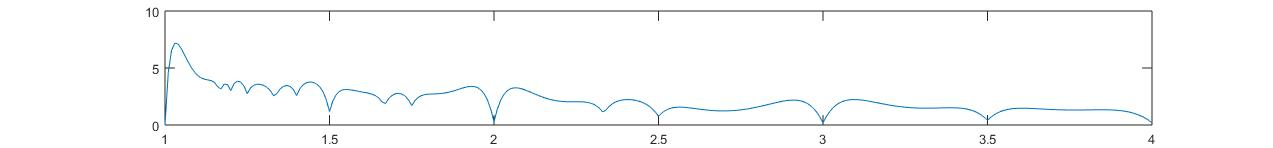
\includegraphics{500Hz-1-7.jpg}
%	    \caption{Caption}
%	\end{figure}
	 
    \begin{center}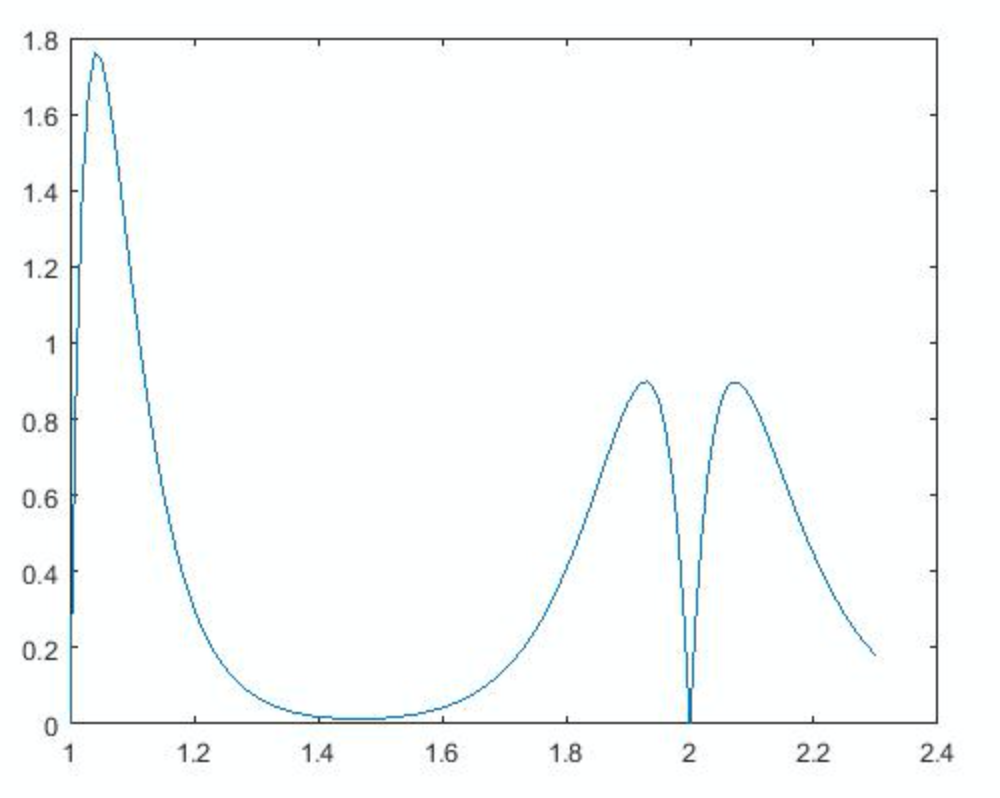
\includegraphics[scale=.5]{1_2.png}
	
	Esta imagen se corresponde con un espectro armónico con 2 parciales.\end{center}
	
    \begin{center}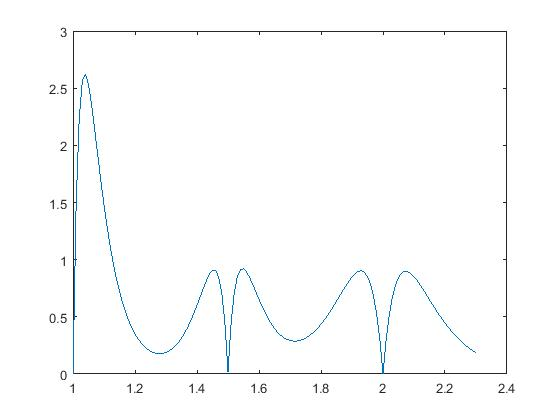
\includegraphics[scale=.5]{Espectro1_3.jpg}
	
	Esta curva se corresponde con un espectro armónico de 3 parciales.\end{center}
	
	\begin{center}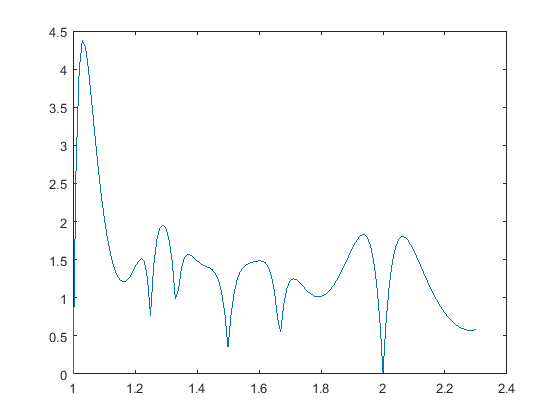
\includegraphics[scale=.65]{Espectro1_5.png}
	
	Curva de espectro armónico de 5 parciales.\end{center}
	
    \begin{center}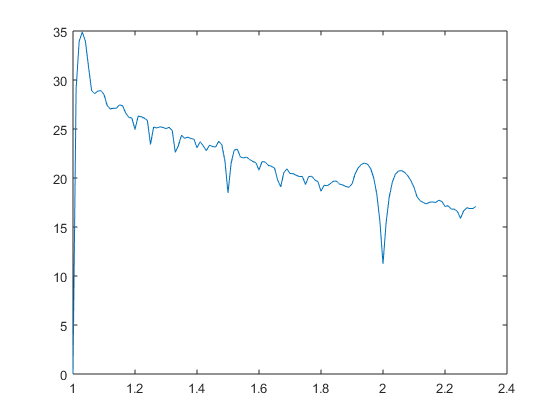
\includegraphics[scale=.65]{Espectro1-20.png}
	
	Curva de espectro armónico de 20 parciales.\end{center}
	
	\begin{center}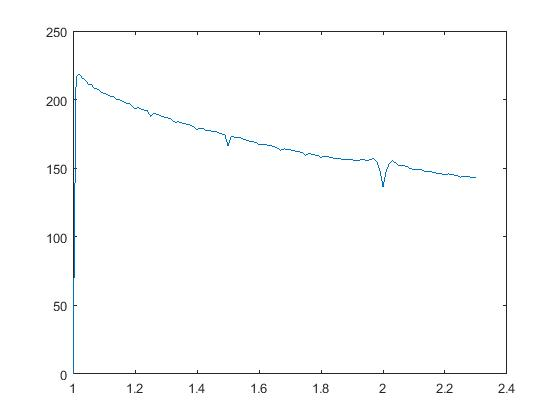
\includegraphics[scale=.5]{Espectro1_50.jpg}
	
	Curva de espectro armónico de 50 parciales.\end{center}
	
%	\begin{center}{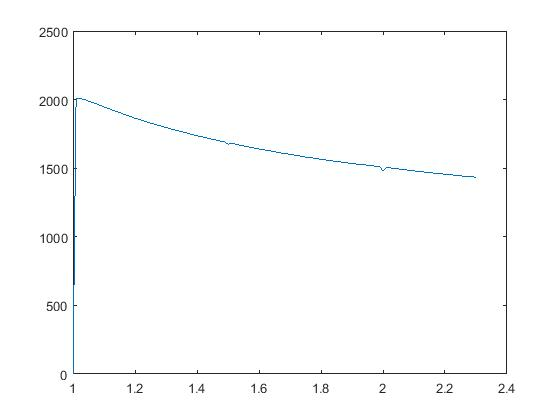
\includegraphics[scale=.5]{Espectros1_150.jpg}
	
%	Curva de espectro armónico de 150 parciales.\end{center}
	\vspace{1cm}
	Observemos los resultados y notemos que cuando las parciales ocupan pocas frecuencias del espectro, un nuevo sonido (de igual espectro pero trasladado en el caso del espectro armónico) será disonante en contadas ocasiones.
	
	\noindent Sin embargo, cuando hay gran cantidad de parciales, la densidad de estas en el conjunto de las posibles frecuencias genera que la disonancia sea muy frecuente. Para pocos valores de $\alpha$ las parciales se alinearán no produciendo gran disonancia.
	
%	El siguiente y último ejemplo es una prueba de este fenómeno sin recurrir a tener un espectro armónico involucrado. El espectro tiene frecuencias múltiplos de $500$, desde $1$ a $1,1$ separadas por un centésima.
	
	
%	\begin{center}{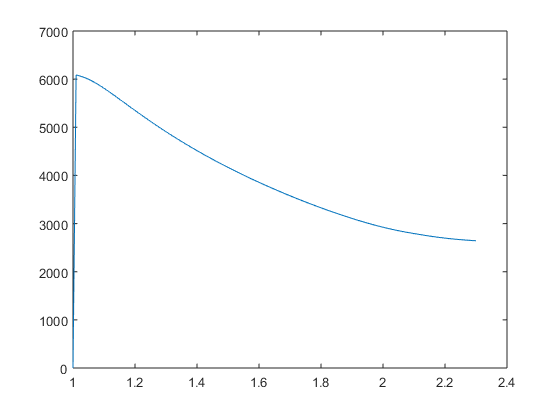
\includegraphics[scale=.5]{Espectro1_.01_1.1.png}\end{center}
	
	
	
	
	
	
	
	
	
	
	
	\newpage
	
%%%%%%%%%%%%%%%%%%%%%%%%%%%%%%%%%%%%%%%%%%%%%%%%%%%%%%%%%%%%%%%%%%%%%%%%%%%%%%	

%\section*{Conclusiones}

%	\newpage
\appendix

\section{Apéndice}
%\appendix

\subsection{Conversión de razones a cents}	
	
El \emph{cent} es una unidad logarítmica de medida utilizada para medir la razón entre dos notas. Fue introducida en Alexander Ellis en 1875 \cite{Bens}. Su principal ventaja frente a utilizar la razón entre las notas es que el cent permite una comparación más rápida entre intervalos. Por ejemplo, a priori podría ser difícil, sin calcularlo explícitamente, saber que nota es más aguda si decimos que la nota $\mathbb{A}$ está a razón $64 / 33$ y la nota $\mathbb{B}$ a $160 / 81$, sin embargo si decimos que están a distancias de 1147 y 1178 cents de una misma nota dada la comparación se vuelve inmediata. 

Otra razón para utilizar los cents es el su carácter aditivo frente al carácter multiplicativo de la razón entre dos notas (por ejemplo, una quinta justa seguido de una tercera justa es una séptima justa, en radios $ \frac{3}{2} \frac{5}{4} = \frac{15}{8} $, en cents $702 + 386 = 1088$)

Los cents fueron introducidos por Ellis, quien establecio que la octava es equivalente a 1200 cents.

Las fórmulas que permiten la conversión son las siguientes:
$$
 c = \left( \frac{1200}{\log_{10} (2)} \right) \log_{10} (r) \approx 3986.314 \log_{10} (r)  
$$
    También:
$$
   c = 1200 \frac{\log_{10} (r)}{\log_{10} (2)} \log_{10} (r) = 1200 \left( \frac{ ( \frac{\ln r}{\ln 10} ) }{( \frac{\ln 2}{\ln 10} ) } \right) = 1200 \left( \frac{\ln r}{\ln 2} \right)
$$
$$
    \boxed{c = 831.7766 \ln r}
$$

donde $r$ es la razón y $c$ su equivalente en cents. De igual modo:
$$\boxed{ r = 10^{ \left(    \frac{c \log_{10} (2)}{1200}    	\right)} \approx 10^{0.00025086 c} } $$

\subsection{La transformada de Fourier}

Cuando en la sección sobre el espectro se hablaba del proceso de descomponer una onda en diferentes armónicos (o componentes fundamenteles de la onda) se hacía referencia a que la maquinaria que permitiría hacer la descomposición sería, en diferentes versiones, el análisis de Fourier. Es esta sección se hará una breve introducción a este análisis centrándose en la llamada \emph{transformada de Fourier}. Conviene que dejar claro que esta sección no pretende fundamentar como o por qué funciona esta clase de herramienta matemática, sino que su objetivo es dar una brevísima pincelada de cómo opera.

El procedimiento fue introducido en 1822 por Jean Baptiste Joseph Fourier como parte de su método para resolver la ecuación del calor (una ecuación en derivadas parciales proveniente de la física matemática) y consiste en escribir una función (que cumpla unas ciertas condiciones, como `por ejemplo que sea periódica) como una combinación lineal de funciones seno y coseno.

Tomaremos como periodo $2 \pi$, así tendremos $ f(\phi + 2\pi) = f(\phi)$. Obviamente solo nos será necesario hacer el proceso en el intervalo semi-abierto $[0, 2\pi)$. Notemos que en el caso de las funciones periódicas seno y coseno ocurre lo siguiente:
$$
	\cos(-n \phi) = \cos(n \phi)  
$$	 
	 
$$	
	\sin(-n \phi) = - \sin(n \phi)	
$$ 
 
En general, podremos escribir una función de la forma:

\begin{equation*}
    \boxed{
        f(\phi) = \frac{1}{2}a_{0} + \sum_{n=1}^{\infty} {a_n \cos(n\phi) + b_n \sin(n\phi)}
    }
\end{equation*}

Donde $a_0,a_n$ y $b_n$ son las denominadas \emph{coeficientes de Fourier}. Sin necesidad de demostrarlas, no es el objeto de este apéndice sino hacer una breve reseña, las fórmulas que los definen son las siguientes:

$$
	a_0 = \frac{1}{\pi} \int_{0}^{2\pi} { f(\phi) } d \phi
$$
 
Para $m>0$:

$$
	a_m = \frac{1}{\pi} \int_{0}^{2\pi} {\cos(m\phi) f(\phi)} d \phi 
$$

$$
	b_m = \frac{1}{\pi} \int_{0}^{2\pi} {\sin(m \phi) f(\phi)} d \phi
$$

Por supuesto cualquier intervalo de longitud $2\pi$, que representa un periodo completo, servirá, por ejemplo, podríamos usar $[-\pi, \pi)$.
En la práctica la variable $\phi$ no representará el tiempo, porque este no tendrá necesariamente un periodo de longitud $2 \pi$. Si el periodo real es de $T$ segundos, entonces la frecuencia fundamental viene dada por $\nu = \frac{1}{T}$ Hz (Herzios, ciclos por segundo). Se hace la siguiente sustitución $\phi = 2\pi \nu t$. Escogiendo $F(t) = f( 2\pi \nu t) = f(\phi)$ y tras realizar las sustituciones pertinentes se obtiene:

$$
	F(t) = \frac{1}{\pi} a_0 + \sum_{n = 1}^{\infty} {(a_n \cos(2n\pi \nu t) + b_n \sen(2n\pi \nu t))}
$$

con las siguientes expresiones para los coeficientes ($m>0$:

$$
	a_m = 2\mu \int_{0}^{T} {\cos(2m \pi \nu t) F(t)} dt
$$

$$
	b_m = 2\mu \int_{0}^{T} {\sin(2m \pi \nu t)F(t)} dt
$$

%pg. 35 

\newpage

\subsection{Problemas de la demostración de Sethares}

    Sethares en un apéndice de su libro ``Tuning, Timbre, Spectrum, Scale'' aporta el siguiente resultado bajo el títilo de \textbf{Teorema 2}:
    
    \textsl{
    Supongamos el timbre $\mathfrak{F}$ con parciales $f_1< f_2 <... < f_n$ separadas todas ellas por al menos $x^{*}$. Entonces $\alpha = 1$ es un mínimo de la curva de disonancia $D_{\mathfrak{F}}(\alpha)$.
    }
    
    
    En esta sección enunciaremos la demostración dada por el autor y haremos incapié en el error en su demostración (plasmada aquí literalmente).
    
\noindent\rule{2cm}{0.4pt}

\noindent\textbf{Demostración:} \\* 
Como $D_{\mathfrak{F}}$ y $D_{\alpha \mathfrak{F}}$ son fijos e iguales para todo $\alpha$, solamente los términos de los sumatorios dobles cambian el valor de $D_{\mathfrak{F}}(\alpha)$.

\noindent Hay $n$ términos en la suma de la forma $d(f_i, \alpha f_i)$ y para cada uno de ellos hay $n-1$ términos de la forma $d(f_i, \alpha f_j), i \neq j$.\\
Mostraremos que el cambio en $d(f_i, \alpha f_i)$  es mayor que $\sum_{ i \neq j}{ d(f_i, \alpha f_j)}$ siempre que $\alpha$ esté suficientemente cerca de 1. \\*
\noindent El cambio en $d(f_1, \alpha f_1)$ para $\alpha \approx 1$ es proporcional a $d'(0)$, $b_2 - b_1$ (porque $\alpha = 1$ se corresponde con $x = 0$).\\*
\noindent El mayor valor posible de $d(f_1, \alpha f_j)$  ocurre cuando $f_1$ y $\alpha f_j$ definen una $x$ con $x = x{**}$.\\
\noindent En este caso tenemos:

\begin{equation*}
    d'(x^{**}) = b_2 (\frac{b_1}{b_2})^{\frac{2 b_2}{b_1 - b_2}} - b_1 (\frac{b_1}{b_2})^{\frac{2 b_1}{b_1 - b_2}}
\end{equation*}

\noindent Como hemos asumido los $f_j$ separados por al menos $x^{*}$ y como $x^{*} = 2 x^{**}$, la siguiente mayor derivada es $d'(3 x^{*})$. 

\noindent Ahora afirmamos que $\sum_{i=0}^{n} | d'(ix^{*}) | < d'(0)$. ($\blacktriangle$) \\*

\noindent Observemos que:

\begin{equation*}
    d'(ix^{*}) = b_2 \left(\frac{b_1}{b_2} \right)^{\frac{ib_2}{b_1 - b_2}} - b_1 \left( \frac{b_1}{b_2} \right)^{\frac{ib_1}{b_1 - b_2}} \equiv b_2 t_2^{i} - b_1 t_1^{i}
\end{equation*}

Y también:

\begin{equation*}
    \sum_{i = 2}^{n}{ | d'(ix^{*}) |} \leq \sum_{i = 1}^{\infty}{ | d'(ix^{*}) |}
\end{equation*}

Como los $d'(ix^{*})$ son del mismo signo, podemos quitar los valores absolutos. Combinando las dos expresiones anteriores llegamos a:

\begin{equation*}
    \sum_{i = 1}^{\infty}{(b_2t–2^{i} - b_1t_1^{i})} = \frac{b_2t_2}{1-t_2} - \frac{b_1t_1}{1-t_1} \equiv t
\end{equation*}

\noindent Siendo aproximadamente $t \approx -0.758$. \\*
\noindent Desde que $f_j$ no necesitan estar espaciados igualmente ("evenly"), $\sum_{i = 0}^{n} \vert d'(·) \vert$ podría estar tan espaciado como $\vert t \vert + \vert d'(x^{**}) \vert \approx 1.05 $.
En el caso general, $d(f_i, \alpha f_j)$, los $\alpha f_j$ podrían ocurrir sobre o bajo los $f_i$. Entonces $\sum_{i = 1}^{n} \vert d'(·) \vert$ podría ser tan grande como $ 2(| t | + | d'(x^{**}) |) \approx 2.1 $.

\noindent En todos los casos, el cambio en los términos en diagonal $d(f_i, \alpha f_i)$ domina la suma de los cambios en todos los términos no diagonales $d(f_i, \alpha f_j)$, dando así la desigualdad requerida.

$\blacksquare$

La hipótesis de la separación mayor que $x_{*}$ es suficiente pero innecesaria. Si $n \leq 7$ los mismos argumentos nos demuestran que la separación entre los $f_i$ no es condicionante, ya que el cambio en cada $d(f_i, \alpha f_i)$ es más de siete veces el mayor valor del cambio en $d(f_i, \alpha f_j)$ para $ i \neq j$ (es decir, $\frac{d'(0)}{d'(x^{**})} \approx 7.7$). 

\noindent\rule{2cm}{0.4pt}

El comentario final nos da la clave: el cambio de la función de disonancia en cerca de $x = 0$ ($\alpha = 1$) es aproximadamente $7.7$ veces mayor que el cambio en el punto donde la derivada es mayor ($x^{**} = 2x^{*}$). \\*

El problema es el siguiente: si yo sumo muchos puntos cercanos a $x**$, el cambio total (la suma de todos los cambios en esos puntos) en la función supera al cambio cerca de $0$. \\*

No es cierto el argumento que da, la afirmación que hace ($\blacktriangle$) es cierta, sin embargo eso no implica que la suma de todos los posibles cambios esté dominada por el cambio en $0$. 

Podemos utilizar muchas herramientas para calcular estos valores y comporbar el error, en mi caso, utilicé R a modo de calculadora. Tomé simplemente suficientes valores separados arbitrariamente pero cercanos a $x^{**}$ como para hacer que el cambio en $0$ fuese más pequeño que el valor absoluto de la suma del resto de cambios. A continuación incluyo el código: \\*

\vspace{2cm} 

\noindent $>$ a = 3.5; b = 5.75 \\*
\noindent $>$ x2 = (2*log(a/b))/(a-b) \\*
\noindent $>$ derivada $<$- function(y) { -a * exp(-a*y) + b * exp(-b*y) } \\*
\noindent $>$ derivada(0) \\*
\noindent [1] 2.25 \\*
\noindent $>$ # este valor es el de la derivada en el punto 0 \\*
\noindent $>$ suma = derivada(x2)+derivada(x2-0.01)+derivada(x2-0.02)+derivada(x2-0.03)+derivada(x2-0.04)+derivada(x2-0.05)+derivada(x2-0.06)+derivada(x2-0.07)+derivada(x2-0.08)+derivada(x2-0.09)+derivada(x2-0.2) \\*
\noindent $>$ suma \\*
\noindent [1] -2.886329 \\*



\newpage

\subsection{Códigos de Matlab}

\subsubsection{Generación de audios}

\%                                                         \%
\%      Generador de audios mediante síntesis aditiva      \%
\%                                                         \%


\newparragraph

\noindent filename = '500 HZ 1-5 5(s).wav';     \% filename = nombre del archivo que generaremos\\*
\noindent sr = 44100;                     \% sr = ratio del muestreo\\*
\noindent time = 5;                       \% time = duraciÛn en segundos de la onda\\*
\noindent espectro = 500 * [1:5];             \% freq = frecuencias de las parciales\\*
\noindent amplitudes = ones( size(espectro) );       \% amp = amplitudes de las parciales\\*
\noindent decay = 0.0005*randn(1,5);      \% decaimiento\\*
\noindent t = 0 : 1/sr : time;
\noindent wave = 0*ones(size(t));


\noindent for i = 1 : length(espectro)\\*
\noindent  env = exp(-abs(decay(i)/time)*[1:length(wave)]);\\*
\noindent  wave = wave+amplitudes(i)*env.*sin(2*pi*espectro(i)*t+2*pi*rand);\\*
\noindent end


\noindent wavwrite(wave,sr,filename)

\subsubsection{Generación de curvas de disonancia}

El programa consta de dos archivos, el primero llamado ``MedidaDisonancia.m'' es una función que retorna la disonancia de una vector de amplitudes y el segundo, llamado ``Principal.m'', la función principal del programa (que utilizará el primero de los archivos para generar las curvas y dibujarlas).

$$
\boxed{
\textnormal{MedidaDisonancia.m}
}
$$

\noindent function d = MedidaDisonancia(espectro,amplitude)\\*

\noindent\% \\*
\% Partiendo de un vector de parciales y otro con sus respectivas \\*
\% amplitudes, esta función calcula la disonancia \\*
\% \\*

\noindent Dstar = 0.22; \\*
\noindent S1 = 0.0207;\\*
\noindent S2 = 18.96; \\*
\noindent A1 = -3.51;\\*
\noindent A2 = -5.75;\\*

\noindent reescalado = 5.58;     \% Factor de reescalado de la curva de disonancia\\*

\noindent N = length(espectro);  \% Número de parciales del espectro\\*

\noindent [espectro,ind] = sort(espectro);  \% Ordenamos el espectro y obtenemos un vector de índices\\*
\noindent ams = amplitude(ind);\\*

\noindent D = 0;\\*

\noindent for i=2:N\\*
\noindent   Fmin = espectro(1:N-i+1);\\*
\noindent   S = Dstar./(S1*Fmin+S2);\\*
\noindent   Fdif = espectro(i:N)-espectro(1:N-i+1);\\*
\noindent   a = min(ams(i:N),ams(1:N-i+1));\\*
\noindent   Dnew = reescalado * a.*(exp(A1*S.*Fdif) - exp(A2*S.*Fdif));\\*
\noindent   D = D + Dnew*ones(size(Dnew))';\\*
\noindent end\\*

\noindent d = D;\\*







$$
\boxed{
\textnormal{Principal.m}
}
$$

\noindent\%                                          \\*
\%              RUTINA PRINCIAL            \\*
\%                                          \\*

\noindent frecuenciaFundamental = 500; \% Frecuencia de la fundamental del espectro en Hz \\*
\noindent topeParcial = 7; \% Máxima razón que incluiremos en el espectro armónico \\*

\noindent espectro = frecuenciaFundamental *[1:1:topeParcial]; \\*
\noindent amplitudes = ones(size(espectro));      \% Creamos un vector de amplitudes (de valor 1) par cada una de las parciales del espectro \\*

\noindent range = 4;         \% Límite de nuestra curva de disonancia \\*
\noindent inc = 0.01;        \% Tamaño del paso \\*
\noindent diss = [0];

\noindent\% \\*
\% Llamamos a la función 'MedidaDisonancia' para cada intervalo \\*
\% \\*

\noindent for alpha=1+inc:inc:range, \\*
\noindent   f = [espectro alpha*espectro]; \\*
\noindent   a = [amplitudes, amplitudes]; \\*
\noindent   d = MedidaDisonancia(f, a); \\*
\noindent   diss = [diss d]; \\*
\noindent end \\*

\noindent plot(1:inc:range,diss) \\*

\newpage

%%%%%%%%%%%%%%%%%%%%%%%%%%%%%
%                      BLIBIOGRAFÍA:                               %
%%%%%%%%%%%%%%%%%%%%%%%%%%%%%
\addcontentsline{toc}{section}{Referencias}
\begin{thebibliography}{ABC9999}

\bibitem[Akk]{CA}
C. Akkoç
``Non-Deterministic Scales Used in Tradicional Turkish Music''
    \textit{Journal of New Music Research} \textbf{31} Nª4, Swets and Zeitlinger (2002)

\bibitem[ANSI]{ANSI}
American National Standards Institute
	\textit{USA Standard acoustic terminology}, S1.1 1960

\bibitem[Ben]{Bens}
D.\,J. Benson,
\textit{Music: A Mathematical Offering}, 
Cambridge University Press, 2008.
%http://www.maths.abdn.ac.uk/∼bensondj/

\bibitem[BW]{BW}
E.\,M. Burns y W.\,D. Ward
``Intervals, scales, and tuning''
    \textit{The Psychology of Music}, Diana Deutsch, Academic Press, New York (1982)

\bibitem[GS]{GS}
X. Gràcia y T. Sanz-Perela,         %Xavier Gràcia y Tomás Sanz-Perela,
``The wave equation for stiff strings and piano tuning'',
\textit{Reports@SCM} \textbf{3} (2017) 1--16

\bibitem[Hal]{H}
D.\,H. Hall,
``The difference between difference tones and rapid beats'',
	\textit{Am. J. Physics, 49} \textbf{7} (July, 1974)
	
\bibitem[Har]{LS}
L. Harrison
    \textit{Lou Harrison's Music Premier}, Peters, NY (1971)

\bibitem[Her]{EH}
E. Herrera %Enric Herrera
	\textit{Teoría musical y armonía moderna, Vol.1}, Antoni Bosch editor, 1995
	
\bibitem[PD]{PD}
R.\,L. Pratt y P.\,E. Doak
	\textit{A subjetive rating scale for timbre}, Journal of Sound and Vibration 45, 317 (1976)

\bibitem[PL]{PL}
R. Plomp y W.\,M. Levelt
``Total Consonance and Critical Bandwidth''
    \textit{Institute for Perception TVO-TNO}, Soeslerberg, Nethrlands (1965)

\bibitem[Set]{Set}
W. Sethares,
\textit{Tuning, Timbre, Spectrum, Scale}, 2nd ed,
Springer, 2005.

\bibitem[Set']{AT}
W.\,A. Sethares
``Adaptative tunings for musical scales'',
\textit{J. Acoustic Society of America} \textbf{96} (July, 1994)

\end{thebibliography}
\end{document}

%% completas secciones 

